\documentclass[a4paper,fleqn]{cas-sc}
 \usepackage{ulem} %Eliminar luego
 
%\usepackage[numbers]{natbib}
\usepackage[authoryear]{natbib}
\usepackage{xcolor}
%\usepackage[authoryear,longnamesfirst]{natbib}
\usepackage{graphicx}
\usepackage{adjustbox}
\usepackage{todonotes}
\usepackage[T1]{fontenc}
\usepackage{verbatimbox}
\usepackage{graphics}
\usepackage{physics}
\usepackage{supertabular}
\hypersetup{
    colorlinks=true,
    linkcolor=blue,
    filecolor=magenta,      
    urlcolor=blue,
}
\usepackage{xr-hyper}
\usepackage{hyperref}

%\externaldocument[supp-]{../supplementstuff.tex}
\usepackage{cleveref}

\makeatletter
\newcommand*{\addFileDependency}[1]{% argument=file name and extension
  \typeout{(#1)}
  \@addtofilelist{#1}
  \IfFileExists{#1}{}{\typeout{No file #1.}}
}
\makeatother

\newcommand*{\myexternaldocument}[1]{%
    \externaldocument{#1}%
    \addFileDependency{#1.tex}%
    \addFileDependency{#1.aux}%
}


%\externaldocument[supp-]{supplementstuff}
\myexternaldocument{supplementstuff}

%\usepackage{xr}
\newcommand{\beginsupplement}{
    \setcounter{section}{0}
    \renewcommand{\thesection}{S\arabic{section}}
    \setcounter{equation}{0}
    \renewcommand{\theequation}{S\arabic{equation}}
    \setcounter{table}{0}
    \renewcommand{\thetable}{S\arabic{table}}
    \setcounter{figure}{0}
    \renewcommand{\thefigure}{S\arabic{figure}}
    \newcounter{SIfig}
    \renewcommand{\theSIfig}{S\arabic{SIfig}}}

\usepackage{comment}

\usepackage{gensymb}
\usepackage{booktabs}
\usepackage{adjustbox}
\usepackage{lscape}
\usepackage{subcaption}
\usepackage{caption}
\usepackage{multirow}
\usepackage{algorithm}
\usepackage{algpseudocode}
\usepackage{booktabs}
\usepackage{amssymb}
\usepackage[utf8]{inputenc}
\usepackage{color}
\usepackage{amsmath}
\usepackage{lineno}
\usepackage{setspace}
%\doublespacing

\usepackage[para,online,flushleft]{threeparttable}
\usepackage{makecell}
%%%Author macros
\def\tsc#1{\csdef{#1}{\textsc{\lowercase{#1}}\xspace}}
\def\code#1{\texttt{#1}}
\tsc{WGM}
\tsc{QE}
\tsc{EP}
\tsc{PMS}
\tsc{BEC}
\tsc{DE}
%%%
%\linenumbers

\begin{document}
\let\WriteBookmarks\relax
\def\floatpagepagefraction{1}
\def\textpagefraction{.001}
\shorttitle{A firebreak placement model using two-stage stochastic programming}
\shortauthors{M. Vilches et~al.}
%\begin{frontmatter}

\title [mode = title]{A two-stage stochastic programming approach incorporating spatially-explicit fire scenarios for optimal firebreak placement} 

\author[2]{Mat\'ias Vilches}[]
\ead{matias.vilches.a@usach.cl}

\author[1,5]{Jaime Carrasco}[orcid=0000-0003-4123-4228]
\ead{jcarrascob@utem.cl}

%\credit{Conceptualization; Investigation; Methodology; Visualization; Writing - original draft}

\author[2,4]{Sebasti\'an D\'avila-G\'alvez}\cormark[1]
\ead{sebastian.davila@usach.cl}

%\credit{Data curation;  Writing; Review.}

%\author[5]{David Palacios}[]
%\ead{david.palacios@ug.uchile.cl}

%\credit{Data curation; Review}

\author[2,4]{Franco Quezada}[]
\ead{franco.quezada@usach.cl}

%\credit{Data curation; Review}

\author[3,5]{Andr\'es Weintraub}[]
\ead{aweintra@dii.uchile.cl}

%\credit{Supervision; Review}

\address[1]{Departamento de Industria, Facultad de Ingenier\'ia, Universidad Tecnol\'ogica Metropolitana, Santiago, Chile}

\address[2]{Industrial Engineering Department, Faculty of Engineering, University of Santiago of Chile, Santiago, Chile}

\address[3]{Industrial Engineering Department, University of Chile, Santiago, Chile}

\address[4]{Program for the Development of Sustainable Production Systems, Faculty of Engineering, University of Santiago of Chile, Santiago, Chile}

\address[5]{Complex Engineering System Institute - ISCI, Santiago, Chile}

\cortext[cor1]{Corresponding author}



%%% ABSTRACT
\begin{abstract}
    Ensuring the effective placement of firebreaks across the landscape is a critical issue in wildfire prevention, as their success relies on their ability to block the spread of future fires. To address this challenge, it is essential to recognize the stochastic nature of fires, which are highly unpredictable from start to finish. The issue is closely linked to the wider problem of climate change, which is causing more frequent and severe wildfires worldwide due to rising temperatures and changing rainfall patterns. Determining the optimal placement of firebreaks in a landscape is a stochastic combinatorial optimization problem that involves the interplay of different management options with the possibilities of a random variable representing the spread of fires, which is currently not well understood. To tackle this issue, our research presents a two-stage stochastic programming approach to model uncertainty in the spread of fires. We thus propose a mixed-integer linear programming formulation to determine the placement of firebreaks, taking into account both the minimization of the expected loss due to wildfires and the expected loss in worst-case scenarios measured based on the Conditional Value-at-Risk function. We assess the effectiveness of our proposed solutions by comparing their performance with random plans, where our preliminary numerical results indicate an average reduction of 5\% and 9\% in the expected burned area and the average of the 10\% most intense wildfires, respectively.
\end{abstract}


\begin{keywords}
Firebreak placement \sep Spatially-explicit fire scenarios \sep Two-stage stochastic programming \sep Wildfire simulation \sep Widlfire management
\end{keywords}


\maketitle

\newpage

\section{Introduction}
\label{sec1}
The available evidence suggests that the frequency and severity of large wildfires, as well as fire-weather conditions, are increasing as a result of human-induced warming \citep{jones2020climate,westerling2016increasing}, which in turn has had a negative impact on both biodiversity \citep{keeley2019fire,kelly2020fire,miranda2023widespread} and human health through erosion, smoke release and greenhouse gas emissions, among other effects \citep{delfino2009relationship,dennekamp2011effects,johnston2009bushfires,johnston2012estimated}. Given these alarming trends, it has become imperative to adopt not only reactive measures but also preventive ones to address the current unfavorable conditions and foster fire-resilient landscapes.

Among the various preventive measures that can be applied in a forest landscape, one is to place firebreaks across it. This involves identifying suitable areas and replacing existing vegetation with non-flammable material, and thus if a future fire reaches these areas, the firebreaks will act as a barrier, blocking the fire's progress. Natural firebreaks can also be present in a landscape, such as rocks, lakes, rivers, canyons, etc. Both natural and human-made barriers can impede the spread of wildfire and can act in combination. The implementation of fuel management techniques allows the creation of artificial barriers. According to \cite{agee2000use}, using firebreaks will alter fire behavior, limiting both the sizes of wildfires and reducing the severity of damage from them. Moreover, fire patterns can be modified by land cover design and proper forest and vegetation management \citep{amiro2001fire,kim2009spatial,cheney1993influence,carrasco2023firebreak}. However, a fundamental question that thus arises is how to place them strategically across a landscape. Current research focuses on the field of preventive management, specifically on finding the best possible placement of firebreaks to minimize the impact of wildfire on the landscape using two-stage stochastic programming.

Operations Research (OR) has addressed this problem in a number of ways, but the application of these models to wildfire management is relatively recent \citep{martell2007forest}. Numerous studies have integrated basic fire ignition and propagation models into spatially explicit integer and dynamic programming frameworks (e.g., \cite{bettinger2009, kim2009spatial, konoshima2008spatial, gonzalez2011integrating}). More sophisticated approaches integrate the element of fire uncertainty through stochastic linear programming (SLP), which introduces randomness into various parameters, including factors like fuel moisture content, treatment costs, and meteorological variables (such as temperature, humidity, wind speed and direction, precipitation, and atmospheric stability). This incorporation of randomness serves to address the inherent uncertainties tied to fire behavior and weather conditions. For instance, \cite{boychuk1996multistage} developed a multistage stochastic programming model for sustainable timber supply at the forest level, incorporating fire risk through probability distributions to estimate the likelihood and potential impact of fire events and the effectiveness of different fire management strategies. Meanwhile, \cite{kabli2015stochastic} proposed a two-stage stochastic programming model to optimize fuel treatment decisions in forest management. In that paper, the authors used probabilistic distributions to represent uncertainty in fire ignition and spread and generated different scenarios to assess fire risk and treatment effectiveness.

A commonly used parameter in wildfire management and OR models is burn probability (BP), which is typically determined through an iterative and concatenated process of simulating spatially explicit fire ignition and growth scenarios across the landscape \citep{parisien2005mapping,finney2005challenge}. Specifically, BP is calculated as the percentage of simulations where a fire reaches a specific point or area \citep{parisien2005mapping}. Wildfire simulation models such as FARSITE \citep{finney1998farsite}, Burn-P3 \citep{parisien2005mapping}, and Cell2Fire \citep{pais2021cell2fire} are capable of generating multiple fire spread simulations and calculating burn probability. BP models have been used to support fuel reduction strategies such as prescribed burns and firebreaks by identifying areas where fuel reduction efforts will have the greatest impact on reducing burn probability \citep{carrasco2023firebreak,ager2010comparison,oliveira2016assessing}.

The placement of effective firebreaks at the landscape scale is a fascinating challenge for decision support modeling, representing an open problem in the fields of Natural Resources and Operations Research in Forestry \citep{martell2007forest,ronnqvist2015operations}. This challenge persists due to several unaddressed aspects, mainly resulting from i) the common focus on simple forest landscapes; ii) the use of simplified fire spread simulators that allow for multiple simulations but potentially sacrifice accuracy over extensive landscapes \citep{bettinger2009,kim2009spatial,konoshima2008spatial,gonzalez2011integrating}; iii) BP-based models provide point estimates of wildfire probability for individual pixels, ignoring confidence bounds and spatial correlations between adjacent pixels \citep{kuhlmann2015generating}. From our perspective, a firebreak plan should have a high probability of spatially overlapping with future wildfire events, and its effectiveness will depend on it. Therefore, to advance firebreak placement strategies, it is critical to address these limitations and encourage innovative approaches that encompass the complexity of real-world scenarios and contribute to more robust and effective fire management strategies. 

\textcolor{red}{Yemshanov et al.~\citep{yemshanov2025graph} propose a graph-based optimization framework for firebreak planning in wildfire-prone landscapes based in Vilches et al.~\citep{vilches2023two}. The formulation considered by Yemshanov et al.~\citep{yemshanov2025graph}  minimizing expected wildfire losses while introducing several modeling extensions. In particular, the constraint limiting the percentage of cells occupied by firebreaks is generalized into a budget constraint that directly controls the number of firebreaks that can be implemented. Additionally, the model incorporates a spatial contiguity constraint to prevent isolated firebreak cells, requiring that each selected firebreak cell be adjacent to at least one other firebreak cell. Furthermore, the authors proposed an alternative formulation to represent that a cell to be reached by fire from multiple neighboring cells.}

In this paper, we present a novel approach based on a two-stage stochastic programming framework to address firebreak placement. This model represents a pioneering step by introducing spatially explicit fire scenarios generated through a simulator that incorporates a fire behavior system, which has not been done before. Specifically, our framework takes into account the uncertainties related to wildfire behavior, incorporating simulations from Cell2Fire, integrated through the directed graph associated with the fire, into the two-stage stochastic programming model. Initially, we focus on minimizing the expected value of the burned forest area, which generally yields satisfactory results. However, we acknowledge its limitations in unfavorable scenarios. To address this, we propose incorporating risk measures into the problem modeling, either by including terms in the objective function to measure risk exposure and mitigate undesirable outcomes or by constraining the feasible solution space to limit the probability and magnitude of adverse events. In this context, we suggest incorporating Conditional Value-at-Risk (CVaR) into the two-stage programming model to account for the probabilistic nature of wildfires and enable more robust decisions regarding firebreak placement. 

The remaining part of this paper is organized as follows. Section~\ref{sec2} provides a theoretical background and introduces the basic notations and assumptions for the problem. In Section \ref{s:general-model}, we introduce a two-stage stochastic programming formulation for the problem. Computational experiments and results are presented in Section~\ref{S:4}. Finally, the conclusions and directions for further work are discussed in Section~\ref{Sec:conclusions}.

\section{\textcolor{brown}{Theoretical Framework to FPP under Uncertainty}}\label{sec2}

In this section, we introduce the basic notations, assumptions, and wildfire concepts to formulate the \textit{firebreak placement problem} (FPP) as a stochastic optimization model.

\subsection{Theoretical Background}
The landscape is represented as a collection of cells denoted by $\mathcal{V}$, automatically determined by the resolution of the data layers (georeferenced ASCII files to include landscape information such as forest fuels, elevation, slope, and aspect). These cells form the nodes of $c$, the graph depiction of the landscape (see Fig.\:\ref{fig:graphs_landscape}-\textbf{A}). In this context, $\mathcal{E}$ represents the set of edges, with each cell having eight neighbors. To allow decision-makers to prioritize protection for specific areas with high priority or value-to-protect (e.g., a biodiversity index), we introduce a parameter $w_v$ for each $v \in \mathcal{V}$, which represents the relevance of each cell $v \in \mathcal{V}$ in the landscape. Similarly, the edges in the graph can represent both the underlying connectivity or other factors, such as distances between cell centers and transportation costs, among other possibilities \citep{carrasco2023firebreak}.

As mentioned in our Introduction, uncertainty arises from the occurrence of fires in the landscape, primarily divided into two coupled processes: ignition and fire spread. The first process involves randomly selecting a cell where the fire starts, which, depending on the origin of the ignition, natural or human-caused, may consider a uniform spatial probability distribution or a probability model trained using historical ignitions, respectively \citep{carrasco2021exploring}. The second process entails the spatial propagation of the fire, which depends on the heterogeneously distributed vegetation in the landscape, topography, and meteorological conditions. In our study, we will assume that fire ignitions are uniformly distributed across the landscape due to their non-anthropic nature, mainly generated by lightning. Furthermore, the fire spread will be simulated using the Cell2Fire simulator \citep{pais2021cell2fire}. When a fire occurs during a simulation $s \in \mathcal{S}$ -- with $\mathcal{S}$ being the set of simulation\textcolor{brown}{s} -- a messaging process is triggered between the nodes of $\mathcal{F}$ that generates a directed graph $\mathcal{T}^s = (\mathcal{V}^s, \mathcal{E}^s)$, where $\mathcal{V}^s \subseteq \mathcal{V}$ is the set containing all the cells burned during the simulation $s$. The set of edges $\mathcal{E}^s$ is constructed from these signals to represent fire propagation between adjacent cells (see more details in \cite{pais2021downstream}).

Cell2Fire, powered by the Canadian Fire Behaviour Prediction (FBP) System, has the capability to calculate various aspects of fires, including fuel consumption, fire intensity, fire rate of spread, and fire type (surface or crown) \citep{hirsch1996canadian}, based on environmental conditions. Fig.\:\ref{fig:graphs_landscape}-\textbf{A} depicts a simulation example of a wildfire produced with Cell2Fire for a landscape in Canada. In it, we can see different colors for the cells corresponding to different fuel types. Specifically, in FBP,  fuel types correspond to identifiable associations of vegetation/forest elements of distinctive species, size, shape, arrangement, and continuity that will exhibit a certain fire behavior under defined burning conditions \citep{hirschetal}. Seventeen discrete fuel types are currently recognized, which are grouped into coniferous, deciduous, mixed wood forest stands, coniferous logging slash, and open grasslands. Gray is reserved for non-flammable cells such as rocks, lakes, bare soils, etc.. Fig.\:\ref{fig:graphs_landscape}-\textbf{A} also displays the ignition point (black circle) and the perimeter (black solid line) of the arbitrarily chosen fire, along with the propagation lines of the graph $\mathcal{T}^s$. Hereafter, the particular forest depicted in Fig.\:\ref{fig:graphs_landscape}-\textbf{A} will be referred to as \texttt{Sub20}.

\begin{figure}[h]
\centering
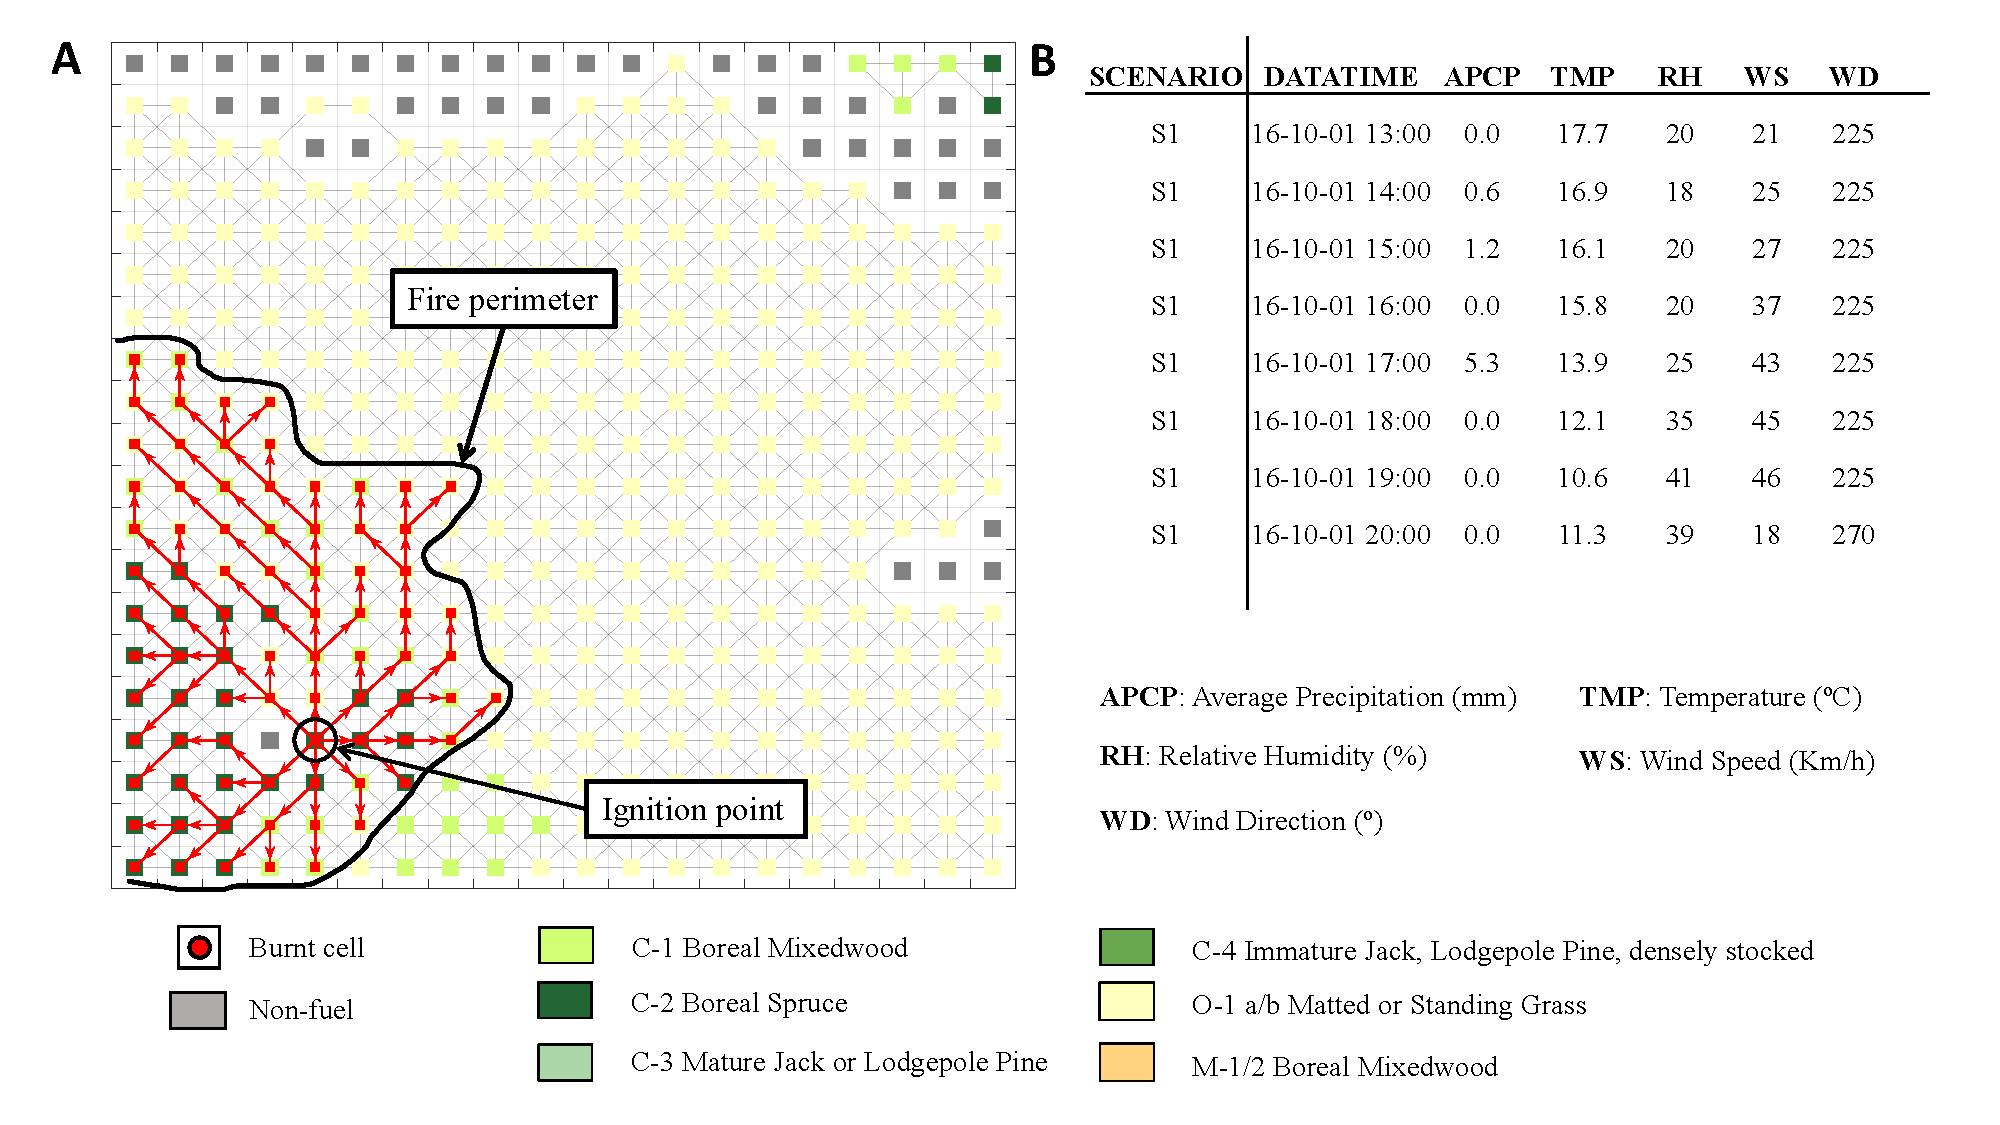
\includegraphics[scale=.5]{figs/example1_sub20_and_weather.pdf}
\vspace{1ex}
\caption{\textbf{A}: Graph representation of the landscape, and a wildfire; \textbf{B}: Example of a fire-weather scenario.}
\label{fig:graphs_landscape}
\end{figure}

\subsection{Feasible solutions}
There is evidence that fire patterns can be influenced by land cover arrangement and appropriate forest and vegetation management practices \citep{amiro2001fire,cheney1993influence}. These activities, referred to as fuel treatment, may involve firebreak creation, prescribed burns, clear-cutting, thinning, or a combination of these methods \citep{North2015ReformFF}. As mentioned above, our study focuses on the problem of firebreak placement, which consists of replacing a number of cells that have forest fuel with a non-flammable one, i.e., it is assumed here that the application of a firebreak to a landscape cell involves the complete removal of vegetation fuel at that location, rendering the firebreaks non-flammable. So, we introduce binary decision variables represented by a vector $ \vb{y} \in \{0,1\}^{\vert\mathcal{V}\vert} $, where $y_v$ equals one if cell $v$ is chosen for constructing a firebreak and zero otherwise. Due to the high costs involved in constructing firebreaks and, broadly, fuel treatments, in practice, only a small percentage of the forest is managed \citep{oliveira2016assessing,jingan2005land}, and that imposes a constraint on the decision variables. Other constraints could be considered, such as environmental restrictions, regulations, access feasibility, and costs, among others. In this first study, the set of feasible solutions is defined  as follows:
\begin{equation} 
    \mathbb{Y} := \{ \vb{y} \in \{0,1\}^{\lvert \mathcal{V}\vert}: \sum_{v\in\mathcal{V}}y_{v}\leq\alpha\lvert \mathcal{V}\vert  \}
    \label{Eq:Constraint}
\end{equation}
where the parameter $\alpha \in [0, 1]$, represents the percentage of the landscape to be treated or \textit{firebreak intensity}.

\subsection{Expected value}
When a fire $\tau$ occurs on the landscape, it affects a number of cells, say $\mathcal{V}^\tau$, and there is a probability that its spread will be blocked by the presence of firebreaks. From this fact, the decision $\vb{y}$ will be as efficient as its ability to intersect the fire $\tau$. Let $ L\left(\vb{y}; \vb{w}, \tau \right) $ be the random variable that represents the burned cells due to a random fire $\tau$ on the landscape $\mathcal{F}$, given the decision variables $\vb{y}$ and the weighted vector $\vb{w}$, from this, we can define the function $\Phi(\vb{y},\vb{w})=\mathbb{E}_\mathcal{\tau} \left[ L \left(\vb{y}, \vb{w}, \tau \right) \right]$ as the expected value (EV) of a random variable $ L\left(\vb{y}, \vb{w}, \tau \right) $ where $\tau$  represents the randomness in our study. Thus, the \textit{firebreak placement problem} (FPP) is formulated as follows:   
\begin{equation} \label{Eq:FMP}
    \min_{\vb{y} \in \mathbb{Y}} \Phi(\vb{y(\vb{w})}):=\mathbb{E}_\mathcal{\tau} \left[ L \left(\vb{y}, \vb{w}, \tau \right) \right]
\end{equation}
The optimization model of Eq.\:(\ref{Eq:FMP}) aim\textcolor{brown}{s} to find a\textcolor{brown}{n} \textit{optimal firebreak plan} $\vb{
y}$ (or simply as an \textit{optimal plan}).
%First, by resolving the following optimization problem, we aim to reduce the expected value (EV) weighted of burned cells:

%where $ L\left(\vb{y}, \vb{w}, \omega \right) $ is the random variable that represents the burned cells due to a random fire $\omega$ on the landscape $\mathcal{F}$, given the firebreak allocation decisions variables $\vb{y}$ and weighted vector $\vb{w}$. 


The distribution of $ L\left(\vb{y}, \vb{w},\tau \right) $ is an unknown function of the vector of decision variables $\vb{y}$ and weighted vector $\vb{w}$, but realizations of $ L\left(\vb{y}, \vb{w}, \tau \right) $ can be observed through simulation experiments with Cell2Fire \citep{pais2021cell2fire}. With this software, we can simulate a set $T := \{\tau_1, \dots, \tau_{\lvert \mathcal{S}\vert}\}$  of independent and identically distributed (i.i.d.) simulations, which generate $L(\vb{y}, \vb{w}, \tau_1),L(\vb{y}, \vb{w}, \tau_2),...,L(\vb{y}, \vb{w}, \tau_{\lvert \mathcal{S}\vert})$ values at any $\vb{y}$ and $\vb{w}$. With them, we can approximate the function $\Phi(\vb{y}, \vb{w})$ by:
\begin{equation} \label{Eq:EVAL}
    \Bar{\Phi}(\vb{y}, \vb{w}) = \dfrac{1}{\lvert \mathcal{S}\vert} \sum_{s=1}^{\lvert \mathcal{S}\vert}L(\vb{y}, \vb{w},\tau_s)
\end{equation}
where the sampling errors can be controlled by increasing the number of i.i.d. simulations $\lvert \mathcal{S}\vert$.

We conclude this section with three important points:
\begin{itemize}
    \item[i)]  $\Phi(\vb{y} = 0,\vb{w})$ represents the expected loss if no fuel treatment action is taken on the landscape and can be approximated by Eq.\:(\ref{Eq:EVAL}). Figure \ref{fig:graphs_landscape}-\textbf{A} illustrates this situation.
    
    \item[ii)] Figure \ref{fig:graphs} illustrates two solutions, denoted as $\vb{y}^1$ (chart \textbf{A}) and $\vb{y}^2$ (chart \textbf{B}). Solution $\vb{y}^2$ proves to be more effective than $\vb{y}^1$ for the wildfire depicted in both tiles, as it prevents the burning of 9 cells in contrast to $\vb{y}^1$ (assuming $\vb{w = 1}$), which prevents three cells. In both cases, firebreaks are first placed in the landscape, followed by a simulation of the fire's progress from the same ignition point and under equivalent weather conditions.

    \item[iii)]  In terms of the function $\Bar{\Phi}$, $\Bar{\Phi}(\vb{y}^1, \vb{w = 1}) = 79 > \Bar{\Phi}(\vb{y}^2, \vb{w = 1}) = 73$. However, for this example, we set $\lvert \mathcal{S}\vert = 1$. In this example, $\vb{y}^2$ is better than $\vb{y}^1$, since it results in a smaller number of burned cells. 
\end{itemize}

\begin{figure}[h]
\centering
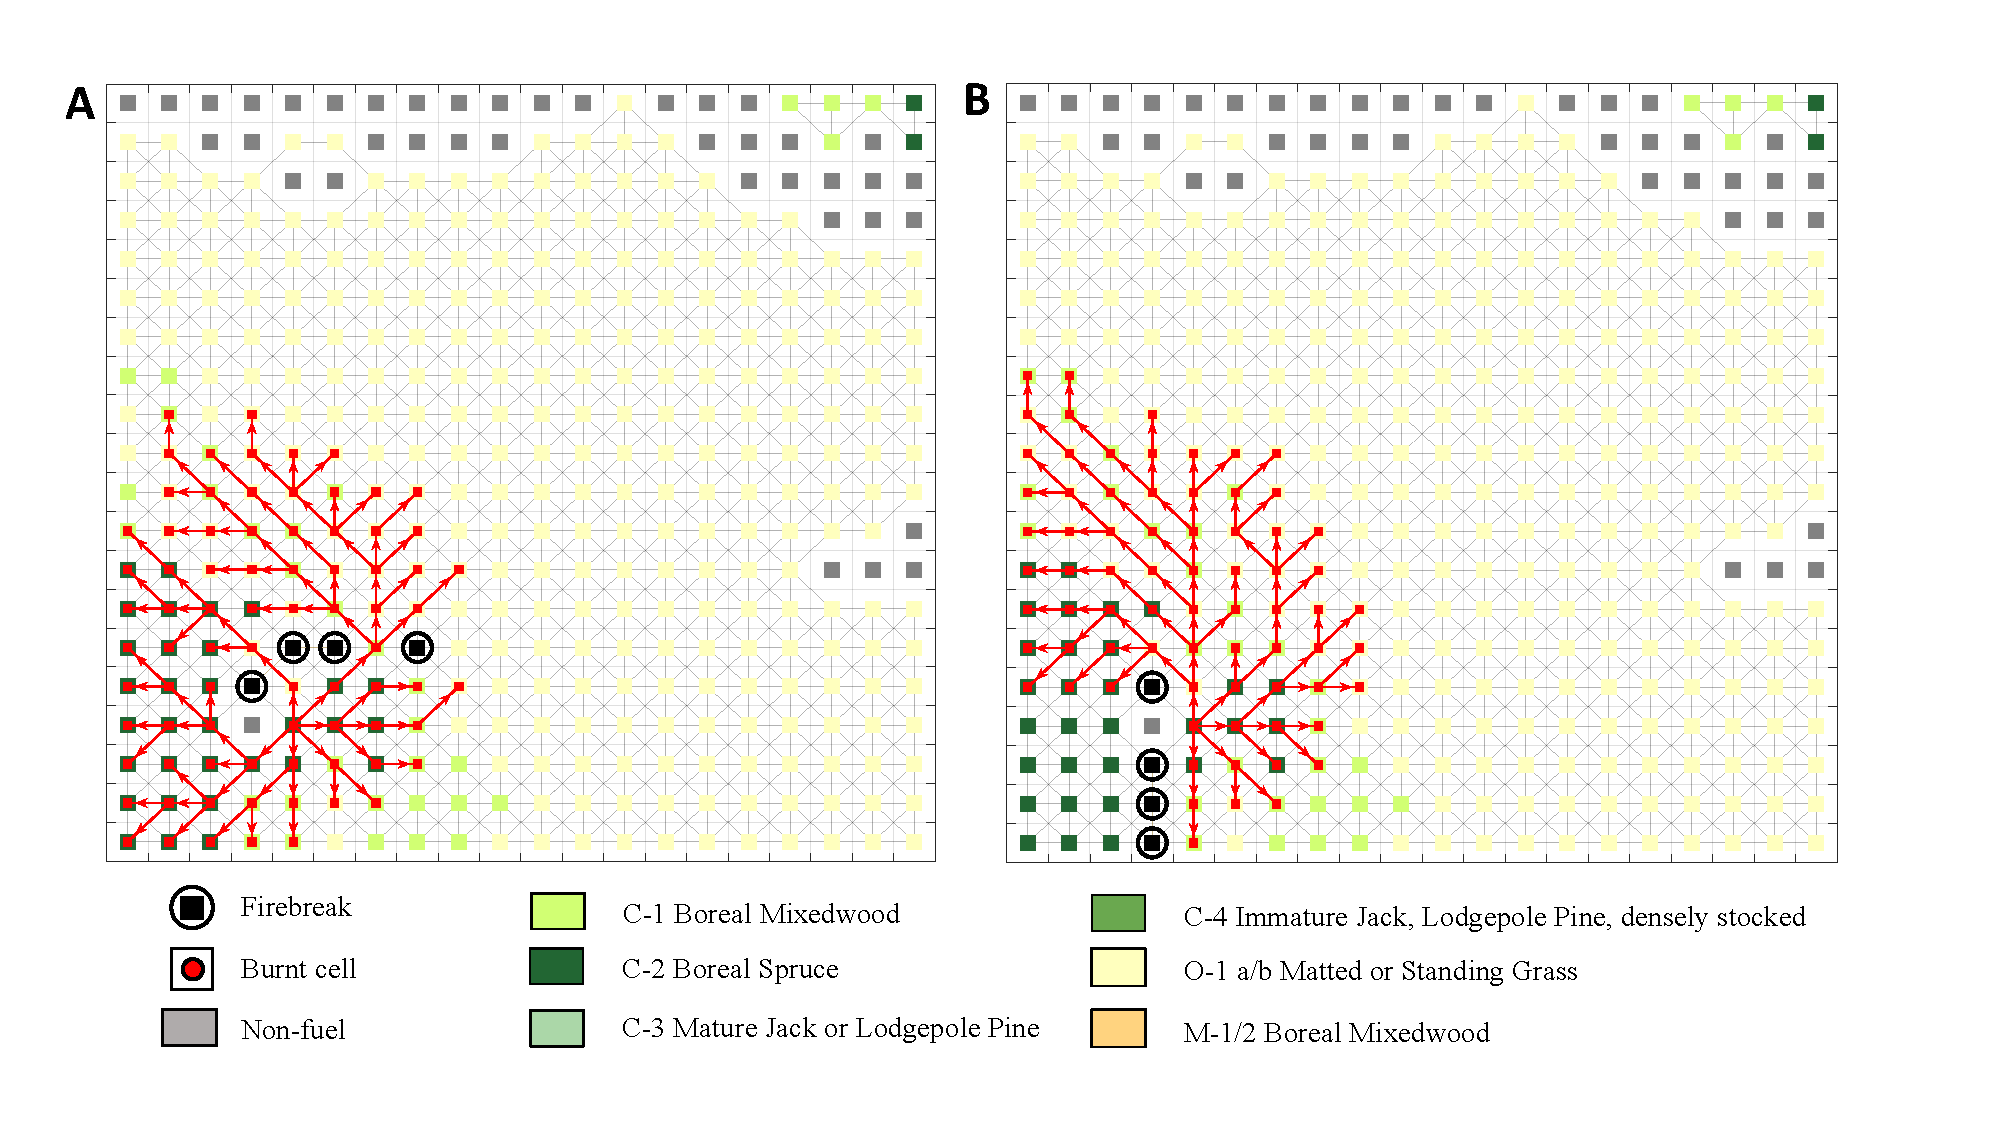
\includegraphics[scale=.5]{figs/example2_efficients_firebreaks.pdf}
\vspace{1ex}
  \caption{The chart \textbf{A} shows a less efficient firebreak placement compared to that depicted in chart \textbf{B}.}
  \label{fig:graphs}
\end{figure}

\subsection{Conditional Value-at-Risk}

Conditional Value-at-Risk (CVaR) is a risk measure that is alternatively known as mean excess loss, mean shortfall, or tail Value-at-Risk (VaR) and is typically used in portfolio theory. Thus, in the FPP context, it can intuitively be seen as the expected value of burned cells in the $( 1 - \beta) \times 100\% $ worst cases, where $\beta \in ]0,1[$. Formally, we follow the paper of \cite{rockafellar2000optimization} to define the CVaR in the context of FPP.

Let $F_L$ be the cumulative probability distribution of our random variable $L := L(\vb{y}, \vb{w}, \tau)$:
\begin{align}
    F_L(\vb{y}, \vb{w}, \varphi) = \mathbb{P}( \{ \tau \in \Gamma : L(\vb{y}, \vb{w}, \tau) \leq \varphi \}).
\end{align}
The Value-at-Risk at level $\beta$, or VaR$_{\beta}$, of  $L$ is defined by:
\begin{align}
    \text{VaR}_{\beta}(L)= \min \{\varphi \in \mathbb{R} : F_L(\vb{y}, \vb{w},\varphi) \geq \beta\}, 
\end{align}
$\text{VaR}_\beta(L)$ thus corresponds to the  $\beta$-percentile of the probability distribution of $L$. In the case where $L(\vb{y}, \vb{w}, \tau)$ represents quantities of burned cells weighted, VaR$_\beta(L)$ can be interpreted as the largest possible burned cells that may be observed once the $(1-\beta)\times 100 $\% worst potential outcomes have been excluded.  

\noindent The  Conditional-Value-at-Risk at level $\beta$ or CVaR$_{\beta}$ is defined  by:
\begin{align}
\text{CVaR}_\beta(L)= \frac{1}{1-\beta} \int_{\beta}^{1} \text{VaR}_{\gamma}(L) d\gamma
\end{align}

Following the result presented in~\cite{rockafellar2000optimization}, $\text{CVaR}_\beta(L)$ for the FPP can be expressed as the optimal value of the following optimization problem:
\begin{align}
\text{CVaR}_\beta(L) = \min \limits_{\varphi, \vb{y} \in \mathbb{Y}  } \Big \{ \varphi + \frac{1}{1- \beta} \mathbb{E}_\tau[(L(\vb{y}, \vb{w}, \tau) - \varphi)^+] \Big \},
\label{CVaR_Formula}
\end{align}
where $( \bullet )^+ = \max(\bullet, 0)$. This reformulation is widely used to reformulate scenario-based stochastic integer programs involving a CVaR risk measure as mixed-integer linear programs. Likewise, in the expected value, we assume that the random variable $L(\vb{y}, \vb{w},\tau)$ has a finite and discrete set of $S$ possible realizations generated by Cell2fire simulator, each one corresponding to a scenario equally probable $L^s:=L(\vb{y}, \vb{w}, \tau_s)$, the term $\mathbb{E}[(L - \varphi)^+]$ in the CVaR of Eq.~\eqref{CVaR_Formula}, can be replaced by the weighted sum of possible outcomes exceeding the risk level $\varphi$, i.e., $\frac{1}{\lvert \mathcal{S}\vert}\sum_{s=1}^{\lvert \mathcal{S}\vert} (L^s - \varphi)^+$, which can easily be handled by adding a set of linear inequalities in the problem formulation. 

\textcolor{red}{Add more references involving CVaR in Wildfires and also in general context of stochastic programming.}

\section{FPP as a two-stage stochastic programming model}\label{s:general-model}

In this study, we present a novel approach to address the FPP. Our proposed methodology involves a two-stage stochastic mixed-integer linear programming mathematical formulation.  We assume that the underlying stochastic input process has a finite probability space so that the information on the evolution of the uncertain parameters can be represented by a discrete set of scenarios $\Omega = \{ 1,\dots, |\Omega|\}$. The probability for scenario $\omega$ is given by $\rho^\omega$, with a total probability of 1 over all the scenarios, i.e., $\sum_{\omega \in \Omega} \rho^\omega = 1$.

Following the notation introduced in Section \ref{sec2}, $\tau_s$ is the wildfire scar resulting from a simulation $s$ of the Cell2Fire. It is characterized by a directed acyclic graph $\mathcal{T}^s=(\mathcal{V}^s,\mathcal{E}^s)$, which represents a possible scenario in the two-stage stochastic program. Let $v(\omega)$ be the node that denotes the ignition point of scenario $\omega$, i.e., the node that begins to spread the wildfire. Thus, we can define the  stochastic problem scenario $\omega$ as a set of nodes $V^\omega$, an ignition point $v(\omega)$ and  the wildfire spread $\delta^\omega_+(v)$ from one node to another, where $\delta^{\omega}_{+}(v)$ denote the set of nodes that are incident from node $v \in \mathcal{V}^\omega$,  following the simulation of the Cell2Fire.

In this approach, the first stage is to decide the firebreak placement, i.e., determining which set of cells will be treated, subject to $\alpha$, which represents the percentage of land to be used as firebreak selected by the decision-maker. Thus, we introduce a binary variable $y_v$ that takes the value 1 if the node $v \in \mathcal{V}$ is placed a firebreak and 0 otherwise. Meanwhile, in the second stage, the performance of these firebreak placements is evaluated in each scenario. Specifically, given the location of the firebreak determined in the first stage, the second stage calculates the number of burned cells in each scenario, taking into account the spread of wildfire simulated. Thus, let $x^\omega_v$ be a binary variable that takes value 1 if node $v \in \mathcal{V}^\omega$ is burned in the scenario $\omega$ after the firebreak placement and 0 otherwise. So the value of $L^\omega(\vb{y},\vb{w},\tau_s)$ can be calculated as $\sum_{v \in \mathcal{V}} w_{\textcolor{brown}{v}} x_v^{\omega} $. The objective is to balance the optimization of the expected value (EV) and the conditional value at risk (CVaR) of the burned cell. Thus, we introduce the parameter $\lambda \in [0,1]$ to balance the trade-off between both objectives. By incorporating EV and CVaR into the optimization process, we aim to enhance the effectiveness and efficiency of firebreak placement strategies. This approach allows decision-makers to study different balances between these two objectives.  \\

Thus, it follows that the mathematical model can be expressed in the following manner:
\begin{subequations} \label{m:fpp}
\begin{align}
\underset{\vb{x},\vb{y},\varphi, \vb{\eta}}{\text{minimize}} \quad &  \lambda \sum_{\omega \in \Omega} \rho^\omega \sum_{v \in \mathcal{V}}w_v x_{v}^{\omega}  + (1-\lambda) \left (\varphi + \frac{1}{(1-\beta)} \sum_{\omega \in \Omega} \rho^\omega\eta^\omega \right)& \label{fo:min_expected4}
\end{align}
\begin{align}
    \text{subject to: } 
    & \sum_{v \in \mathcal{V}} y_{v} \leq \alpha \lvert \mathcal{V} \vert,& \label{c:capacity}\\
    & x_{v(\omega)}^{\omega} = 1 & \forall \omega \in \Omega, \label{c:ignition} \\
    & x_{v}^{\omega} \leq x_{u}^{\omega} + y_{u} & \forall v \in \mathcal{V},  \; u \in \delta^{\omega}_+(v) \; \omega \in \Omega, \label{c:spread}\\
    %& x_{u}^{s} \leq 1 - y_{u} & u \in V\setminus \{ v(s)\} , \; s \in \mathcal{S}, \label{c:spread_2}\\
    & \sum_{v \in \mathcal{V}^{\omega} }w_v x_v^\omega - \varphi \leq \eta^\omega & \forall \omega \in \Omega, \label{c:cvar_linearization} \\ 
    & \eta^\omega \geq 0 &\forall \omega \in \Omega,  \label{c:eta} \\
    &\varphi \geq 0, & \\    
    & \bf{x}, \bf{y} \in \{0,1\}. \label{c:variables} 
\end{align}
\end{subequations}

Equation\:\eqref{fo:min_expected4} minimizes the linear combination of the expected value of weighted burned nodes and the conditional value at risk. The first term corresponds to the sum of all burned cells \textit{v} weighted by parameter $w_v$ over all scenarios with a certain probability of occurrence $\rho$. Meanwhile, the second term seeks to minimize worst-case scenarios represented by the weighted sum of burned cells over the Value-at-Risk $\varphi$. We introduce the variable $\eta_\omega$ that allows linearization of the formulate \eqref{CVaR_Formula}. In particular, the constraint \textcolor{brown}{\eqref{c:cvar_linearization}} force $\eta_{\omega}$ take the value  $L(\vb{y}, \vb{w}, \tau_\omega) - \varphi$, while the constraint \textcolor{brown}{\eqref{c:eta}} force to take only nonnegative values. \textcolor{red}{Note that the parameter $\lambda$ represents the level of risk aversion of the decision-maker. 
When $\lambda = 0$, the decision-maker is indifferent to risk. 
When $\lambda = 1$, the decision-maker behaves in a risk-neutral manner. 
As the value of $\lambda$ increases, the decision-maker exhibits greater risk aversion.} Constraints \eqref{c:capacity} define the limit of cells used as a firebreak based on the value of $\alpha$. Constraints \eqref{c:ignition} establish the origin of the wildfire, and Constraints \eqref{c:spread} define the propagation of fire in each scenario. This is as follows: given a scenario $\omega$ if the node (or cell) $v$ is burned, an incident node $u$ from node $v$ must also be burned unless a firebreak is allocated. Thus, given a starting ignition node, $v(\omega)$ in each scenario, the firebreaks limit the wildfire spread, and a decision has to be made in every node in which a firebreak can be assigned to stop the fire such that minimizes the objective function. Finally, the constraint \eqref{c:variables} defines the binary variables $\bf{x}$ and $\bf{y}$ declaring that not half harvest can be done at each node. Note that if the firebreak intensity is equal to zero (i.e., $\alpha=0$), the constraints \eqref{c:spread} recover the fire scar of each scenario.

\textcolor{red}{Given the objective function and constraint~\eqref{c:ignition}, it is easy to verify that the integrality constraints on the variable $\mathbf{x}$ can be relaxed. In particular, replacing $\mathbf{x} \in \{0,1\}$ with $0 \leq \mathbf{x} \leq 1$ preserves the optimal integer solution.}

\begin{comment}
\section{\textcolor{brown}{Method solution}}
Benders decomposition, also known as the L-shaped decomposition method, is widely used in two-stage stochastic programming. It partitions the problem into a master problem (handling first-stage decisions) and subproblems (handling second-stage, scenario-specific decisions). Information from subproblems is incorporated via Benders cuts—optimality and feasibility cuts—which guide the iterative refinement of the master problem through a cutting-plane algorithm. When first-stage variables are integer, the method is extended using the Branch-and-Benders Cut (BBC) framework. To address convergence challenges, various enhancements have been developed, including stabilization techniques, adaptive cut aggregation, dual-based cut strengthening, and partial decomposition with representative scenarios. These strategies significantly improve the scalability of Benders decomposition in large-scale applications \citep{rahmaniani2017benders}.

In particular, the Two-Step Benders Decomposition with Scenario Clustering (TBDS) proposed by () solves the two-stage stochastic mixed-integer programs with relatively complete continuous recourse, which means that the first-stage involves integer and continuous variables. TBDS is based on the partial benders decomposition proposed by (), which includes a set $\Omega_{MP}$ of representative or artificial scenarios directly into the master problem.  It is structured around three key components. First, the algorithm defines two hierarchical subproblems: SP1, a linear program derived by fixing the integer first-stage variables to determine all continuous variables, and SP2, which further decomposes the second-stage decisions per scenario based on the SP1 solution. Second, scenario-specific constraints are partially incorporated into the master problem to reduce the generation of weak early-stage solutions. To further mitigate computational burden, the method applies scenario clustering techniques, grouping similar scenarios to limit the number of subproblems while preserving solution diversity. Third, the approach employs Benders dual decomposition to generate strengthened optimality proposed in () and integrates these into a branch-and-cut framework to improve convergence speed. 

In our problem, the clustering process proposal is not suitable because it is based on the optimal solution of each scenario; however, in this case this solution is a bad approximation, because if the number of the firebreak is greater or equal than eight the optimal solution of the fixed one scenario cover the ignition point. Then, we propose an alternative representative scenario selection. Particularly, since the CVaR measure we select the $\mid\Omega_{MP}\mid$-th scenarios with the most burnt nodes before locating the firebreak. 

\begin{proposition}
Let $\mathcal{X}$ be the polyhedron created by constraints \eqref{c:capacity}-\eqref{c:variables}. Then, the extreme points of the $conv_x(\mathcal{X})$ are integers.
\end{proposition}
\begin{proof}
\chgred{the proof is left as an exercise to the reader}
\end{proof}

In addition, note that given a fixed first-stage variable, the second-stage is always feasible because this recalculates the propagation of fire given the firebreak proposed in the first-stage.  

Benders decomposition applies naturally in \eqref{m:fpp} because the variables can be divided into the integer variables $\bm{y}$ and continuous variables $\bm{{x}}$. In the master problem with integer variables, we decide the location of the firebreaks while the subproblems represent the fire spread in each scenario given the firebreaks defined in the master problem.

Later, we define the master problem to the case $\lambda = 1$ that contains the binary variables as follows:


We introduce the auxiliary variables $\Theta$, and $\theta_\omega$, $\forall \omega \in \Omega_{SP}$, which approximates the objective the objective function SP1, and approximates the SP2 subproblem cost, respectively. 

\begin{subequations} \label{m:masterproblem}
\begin{align}
    \underset{\vb{x},\vb{y}}{\text{minimize}} &\; \Theta + \lambda\left(\sum_{\omega \in \Omega_{MP}}\rho^{\omega}\sum_{v \in \mathcal{V}}\omega_v x_v^\omega \right) + (1 - \lambda)\left(\frac{1}{(1-\beta)}\sum_{\omega \in \Omega_{MP}} \rho^\omega \eta^\omega \right) & \\
    s.t. \; 
    & \sum_{v \in \mathcal{V}} y _{v} \leq \alpha|\mathcal{V}|, & \\
    & x_v(\omega)^{\omega} = 1 & \omega \in \Omega_{MP}\\
    & x_v^\omega \leq x_u^\omega + y_u & v \in \mathcal{V}, u \in \delta_+^\omega (v), \omega \in \Omega_{MP}, \label{c:link_xy_bm}\\
    & \sum_{v \in \mathcal{V}^{\omega} }w_v x_v^\omega - \varphi \leq \eta^\omega & \forall \omega \in \Omega_{MP}, \label{c:cvar_linearization_bm} \\ 
    & \Theta \geq (1 - \lambda)\left(\varphi + \frac{1}{(1-\beta)}\sum_{\omega \in \Omega_{SP}} \rho^{\omega}\theta_\omega\right) & \label{c:aggregate-benders-cut}\\
    & \Theta \geq \left( (1-\lambda)\overline{\varphi} +\frac{1}{(1-\beta)}\rho^\omega\eta^\omega + \sum_{v \in \mathcal{V}}(y_v -\hat{y}_v)\pi^*  \right)_i & i \in I, \label{c:aggregate-benders-cut2_bm} \\
    & \theta_\omega \geq \left( \frac{1}{(1-\beta)} \rho^{\omega} \eta^{\omega} + \sum_{v \in \mathcal{V}}(y_v -\hat{y}_v)\hat{\pi}_\omega^* + (\varphi - \hat{\varphi})\mu_\omega^* \right)_i  & \forall j \in J_\omega, \omega \in \Omega_{SP}, \label{c:disaggreagre-benders-cut} \\ 
    & \xi, \xi^\omega, \eta^\omega \geq 0 &\forall \omega \in \Omega,  \label{c:eta} \\
    &\varphi, \bf{x} \geq 0, & \\    
    & \bf{y} \in \{0,1\}. \label{c:variables} 
\end{align}
\end{subequations}

Constraints \eqref{c:aggregate-benders-cut} is called the \textit{subprobem connectivity constraint}. Constraints \eqref{c:aggregate-benders-cut2} and \eqref{c:disaggreagre-benders-cut} are the \textit{optimality cuts}. 

$$
SP1(y^*) = \underset{x,\varphi,\eta}{\min}\left\{\left(\varphi + \frac{1}{(1-\beta)}\sum_{\omega \in \Omega_{SP}} \rho^{\omega}\eta_\omega\right) : \sum_{v \in \mathcal{V}^{\omega} }w_v x_v^\omega - \varphi \leq \eta^\omega, \; \forall \omega \in \Omega_{SP}, \; y = y^*, y \in \mathcal{Y}, \vb{x}^\omega, \eta^{\omega} \in \mathbb{R}_{+}  \right\} 
$$

It the primal subproblem (SP1) returns a feasible solution ($\overline{y},\overline{x},\overline{\eta}$), then the constraint \eqref{c:aggregate-benders-cut2_bm} is added.

$$
SP2(y^*,\overline{x},\overline{\eta},\omega) = \underset{}{\min}\left\{\rho^{\omega}\eta_\omega: \sum_{v \in \mathcal{V}^{\omega} }w_v x_v^\omega - \varphi \leq \eta^\omega, y_\omega = y^*, \eta_\omega = \overline{\eta}, y_\omega \in \mathbb{R}_+^{|\mathcal{V}|,} \right\}
$$

Let $\hat{\vb{y}}$ be a feasible solution of the master problem \eqref{m:masterproblem}, hence we can solve separable subproblems by scenario $\omega \in \Omega$ as follows:

\begin{subequations}\label{m:subproblem}
\begin{eqnarray}
    z_{P}^{\omega}(\hat{y}) := \quad \underset{\vb{x},\vb{y}}{\text{minimize}} & \rho_{\omega} \left( \sum_{v \in \mathcal{V}} w_v x_v \right) & \\
    s.t. & x_{v}^{\omega} \leq x_{u}^{\omega} + \y & v \in \mathcal{V}, \; u \in \delta_{+}^{\omega}(v), \\ \label{c:sp_spreadfire}
    & x_{v(\omega)}^{\omega} = 1, & \\ \label{c:sp_ignitionnode}
    & y_v = \hat{y}_v & v \in \mathcal{V}, \\
    & \sum_{v \in \mathcal{V}} y _{v} \leq \alpha|\mathcal{V}|, & \\
    & \vb{y} \in \{0, 1\}, x_{v} \geq 0 & v \in \mathcal{V}.
\end{eqnarray}
\end{subequations}

Note that given a $\hat{\vb{y}}$ feasible solution of the master problem, the subproblem always generates a feasible solution, then only generates \textit{optimality cuts} for the master problem. In addition, each dual subproblem is represented as:

\begin{subequations}\label{m:dualsubproblem}
\begin{align}
    z_{D}^{\omega}(\hat{y}) := \quad \underset{\vb{\lambda},\vb{\gamma}}{\text{maximize}} & \sum_{v \in \mathcal{V}} \sum_{u \in \delta_{s}(v)} \lambda_{v,u}^{s}\hat{y}_{u} + \gamma_{\omega} & \\
    s.t. & \sum_{u \in \delta_{+}^{\omega}(v)}\lambda^{s}_{v,u} - \sum_{u \in \delta_{-}^{\omega}(v)}\lambda^{\omega}_{v,u}  \leq \rho_{\omega}w_{v} & v \in \mathcal{V}, \\
    & \gamma_{s} \leq \rho_{\omega}w_{v(\omega)}, & \\
    & \lambda_{v,u} \leq 0 & v \in \mathcal{V}, \; u \in \delta_{+}^{\omega}(v).
\end{align}
\end{subequations}

where ($\vb{\lambda}$, $\vb{\gamma}$) are the variables dual of the constraints \eqref{c:sp_spreadfire} and \eqref{c:sp_spreadfire} respectively.

\begin{algorithm}[htbp] 
\caption{Algorithm for Solving Problem \eqref{m:subproblem}}
\label{alg:lp_subproblem_problem}
\begin{algorithmic}[1]
\State \textbf{Require:} $\hat{\bm{y}}$, \; $v(s)$
\State $R = \{v(s)\}, \quad \mathcal{T} = \{v(s)\}, \quad x_v^s = 0 \quad \forall v \in \mathcal{V}^{s} \setminus \{v(s)\}, \quad x_{v(s)} = 1$
\While{$|R| < |\mathcal{V}^{s}|$}
\State $t = \emptyset$
\For{$v \in \mathcal{T}$}
\For{$u \in \delta^{+}_{s}(v)$}
\State $x_u^s = \max\{x_u^s, x_v^s - \hat{y}_u\}$
\State $R \leftarrow R \cup \{u\}, \quad t \leftarrow t \cup \{u\}$
\EndFor
\EndFor
\State $\mathcal{T} \leftarrow t$
\EndWhile
\end{algorithmic}
\end{algorithm}

We follow the bender decomposition proposal for ADD CITE, where a partition of scenarios $\Omega := \Omega_{MP} \cup \Omega_{SP}$ is realized. Then, $\Omega_{MP}$ is incorporated into the Master Problem. In the CVaR formulation, $\phi$ is a linking variable between all scenarios. 

In order to select the $\Omega_{MP}$ scenarios, we take into account the $\kappa$ percentage of the scenarios with the largest scar (i.e., $|\mathcal{V}^\omega|$). 

In order to obtain a separable subproblem a copy $\hat{\phi}$ variable in each subproblem.

In addition, a warm start is a proposal. First, we collapse the graphs in one, where the weight edges represent the number of scenarios using this edge. Later, we select the largest weight outdegree as a firebreak, then recalculate the graph resultants, and repeat the process until we allocate the $\lfloor \alpha |\mathcal{V}| \rfloor$ firebreaks.

We study adding the constraint $\eqref{c:spread}$ as a lazy constraint, i.e., is removed in the root node, and is incorporated along the branch and bound tree when an incumbent solution is infeasible concerning any of these constraints.

\end{comment}

\textcolor{red}{\emph{OPTION 1: equivalence between MBSMP and FPP}}\\
Note that when $\lambda = 1$, the proposed formulation corresponds to a particular case of the 
\textit{Measure-Based Spread Minimization Problem} (MBSMP) introduced in~\citep{taninmics2024benders}. 
The MBSMP considers a stochastic directed network in which each arc $(i,j)$ is associated with a probability of being active. 
If an arc $(i,j)$ is active and the contagion process reaches node $i$, then the spread may propagate to node $j$.

In this framework, labels are assigned to arcs, where each arc has at least one label but may possess multiple labels. 
The decision-maker selects a subset of labels to deactivate, which results in the removal of all arcs associated with those labels. 
The objective is to minimize the expected spread of the contagion over the network.

Although the FPP removes nodes while the MBSMP removes labeled arcs, the two formulations are equivalent under an appropriate labeling scheme. 
Consider the directed graph that represents wildfire propagation. 
If each arc $(i,j) \in \mathcal{E}^{\omega}$ is assigned the label corresponding to its origin node $i$, then placing a firebreak at node $i$ in the FPP is equivalent to deactivating all arcs outgoing from node $i$ in the MBSMP.

Finally, the maximum number of firebreaks allowed in the FPP, given by $\alpha |\mathcal{V}|$, directly corresponds to the label-deactivation budget $B$ in the MBSMP formulation.

\textcolor{red}{\emph{OPTION 2:  equivalence between MBSMP and FPP}}\\
Note that when $\lambda = 0$, the proposed formulation corresponds to a special case of the 
\textit{Measure-Based Spread Minimization Problem} (MBSMP) introduced in~\citep{taninmics2024benders}. 
While the MBSMP deactivates labeled arcs and the FPP removes nodes, the two models are equivalent under a suitable labeling scheme. 
Specifically, assigning label $i$ to each arc $(i,j) \in \mathcal{E}^{\omega}$ makes placing a firebreak at node $i$ equivalent to deactivating all arcs outgoing from $i$. 
The firebreak budget $\alpha |\mathcal{V}|$ in the FPP then corresponds to the label-deactivation budget $B$ in the MBSMP.

\section{Results and discussion}
\label{S:4}

\subsection{\textcolor{brown}{Computational experiments}}
%\textcolor{red}{In this study, we use real landscapes for our experiments, namely \texttt{Sub100}, situated in the Alberta region of Canada. \texttt{Sub20} represents a forest patch covering an area of 400 hectares (depicted in Fig.\:\ref{fig:graphs}), this region is a partition of \texttt{Sub100} that is employed for the assessment of the optimization model. Additionally, for our computational experiments, \texttt{Sub100} is further subdivided into \texttt{Sub40}. The landscape is divided into $100 \times 100$ m$^2$ cells, and their detailed landscape information can be found at \url{https://github.com/fire2a/C2FFBP}. We use Cell2Fire to conduct simulations of multiple wildfires, which requires fire-weather scenarios (FWS) specific to the study area \citep{parisien2005mapping, pais2021cell2fire}. These scenarios encompass crucial factors such as temperature, relative humidity, wind speed, wind direction, and fire weather indices, which are necessary inputs to the FBP system \citep{hirsch1996canadian} (see, e.g., Fig.\:\ref{fig:graphs_landscape}-\textbf{B}). To ensure the representation of extreme conditions, we exclusively considered scenarios that exceeded the 95th percentile mean temperature.}

We employed three real landscapes in our experiments: \texttt{Sub20}, \texttt{Sub40}, and \texttt{Sub100}, all situated in the Alberta region of Canada. The \texttt{Sub20} landscape, a 400-hectare forest patch depicted in Fig.\:\ref{fig:graphs_landscape}, was chosen for assessing computational performance and observing how the objective function evolves with changes in model parameters. To evaluate the model's computational efficacy over larger forest areas, we extended the study to include \texttt{Sub40} (Fig.\:\ref{fig:Sub40}) and \texttt{Sub100} (Fig.\:\ref{fig:Sub100}) under specific parameter configurations. Each landscape is divided into $100 \times 100$ m$^2$ cells, and detailed information about these landscapes can be found at \url{https://github.com/fire2a/C2FFBP}. Simulations of multiple wildfires were conducted using Cell2Fire, requiring fire-weather scenarios (FWS) specific to the study area \citep{parisien2005mapping, pais2021cell2fire}. These scenarios include crucial factors such as temperature, relative humidity, wind speed, wind direction, and fire weather indices—essential inputs for the Canadian Fire Behavior Prediction (FBP) System \citep{hirsch1996canadian} (see, e.g., Fig.\:\ref{fig:graphs_landscape}-\textbf{B}).

The construction of fire-weather scenarios involved historical data obtained from the Climate Information Section of the Agriculture and Forestry website of Alberta, as well as data from the Yaha Tinda Auto station (coordinates: 51.6547°, -115.3617°). This station was selected for its proximity to the coordinates of the forests used in the simulation. To ensure representation of extreme conditions, we exclusively considered scenarios exceeding the 95th percentile mean temperature.

The computational experiments conducted on the \texttt{Sub20} forest were considered to analyze the performance of the mathematical model, the number of scenarios $|\Omega|$, the firebreak intensity $\alpha$, and the parameter $\lambda$. The values chosen for the number of scenarios were $|\Omega| \in \{ 20, 60, 100, 140, 180 \}$. Additionally, our experiments set the $\alpha$ values to 0.01, 0.02, 0.03, 0.04, 0.05 (or 1\%, 2\%, 3\%, 4\%, 5\%, respectively). Lastly, the values assigned to parameter \textcolor{red}{$\lambda$ are $ \{0.0, 0.1, 1.0,10.0,100.0 \}$}. We randomly generated five instances for each combination of $|\Omega|$, $\alpha$, and $\lambda$, resulting in a total of 375 instances. Remark that every individual occurrence is produced by a distinct simulation sample using C2F, which randomly selects various combinations of ignition points and fire-weather conditions.

In order to simplify the analysis, we assigned the same protection priority to every cell; thus, for every node $v \in \mathcal{V}$, we set the value of $w_v$ equal to 1. Also, the parameter $\beta$ was fixed on 0.9, meaning that CVaR will minimize the expected shortfall, which would be the average loss in the 10\% cases where the burned area exceeds its Value-at-Risk.

All procedures and mathematical formulations were implemented using Python programming language v3.10.9. The optimization problems were solved using the GUROBI Optimizer v10.0.2. The experimental procedures were executed on a computational framework featuring 12th Gen Intel(R) Core(TM) i5-12400 processor, with a speed of 2.50 GHz and 3,200 MHz Dual Channel 16 GB of RAM. The computations were performed on the Windows 10 Home 22H2 operating system.

\textcolor{red}{Add statistical characteristics about instances as number of nodes, arcs, degree (maybe in and out-degree), among others. For the scenarios, it is suggest the some dispersion metric of the scenarios or similar.}

\subsection{Computational assessment of the mathematical model}

Extensive computational experiments were conducted to assess the performance of the proposed mathematical model under various scenarios ($|\Omega|$) and values of the $\alpha$ and $\lambda$ parameters. In order to ensure consistent and controlled experimentation, a predetermined runtime limit of 1,800 seconds was set for each instance. These parameters were applied uniformly across all instances of \texttt{Sub20} described above. 

The results are reported in Table \ref{tab:gap_time}. The column denoted as $|\Omega|$ represents the total number of scenarios employed for solving the given instances. The column labeled \texttt{MIP$_{gap}$} provides the gap in percentage between the best lower bound and the best feasible solution obtained during the branch-and-cut algorithm in the GUROBI solver. In addition, the column labeled \texttt{C.TIME[min]} reports the average CPU time in minutes spent. %Note that each experiment was evaluated for various magnitudes of firebreak intensity $\alpha$ and $\lambda$ parameters.

% Please add the following required packages to your document preamble:
% \usepackage{booktabs}
% \usepackage{graphicx}
\begin{table}[h!]
\caption{Average computational time and gap by $\alpha$, number of scenarios, and factor $\lambda$.}
\label{tab:gap_time}
\resizebox{\textwidth}{!}{  %
\begin{tabular}{@{}lrrrrrrrrrrr@{}}
\toprule
\multicolumn{1}{c}{}           & \multicolumn{1}{c}{$\alpha$}          & \multicolumn{2}{c}{1\%}                                  & \multicolumn{2}{c}{2\%}                                  & \multicolumn{2}{c}{3\%}                                  & \multicolumn{2}{c}{4\%}                                  & \multicolumn{2}{c}{5\%}                                  \\ \midrule
\multicolumn{1}{c}{$\lambda$} & \multicolumn{1}{c}{$|\Omega|$} & \multicolumn{1}{c}{\texttt{C.TIME[min]} } & \multicolumn{1}{c}{\texttt{MIP$_{gap}$} } & \multicolumn{1}{c}{\texttt{C.TIME[min]} } & \multicolumn{1}{c}{\texttt{MIP$_{gap}$} } & \multicolumn{1}{c}{\texttt{C.TIME[min]} } & \multicolumn{1}{c}{\texttt{MIP$_{gap}$} } & \multicolumn{1}{c}{\texttt{C.TIME[min]} } & \multicolumn{1}{c}{\texttt{MIP$_{gap}$} } & \multicolumn{1}{c}{\texttt{C.TIME[min]} } & \multicolumn{1}{c}{\texttt{MIP$_{gap}$} } \\ \midrule
\multicolumn{1}{r}{0.0}          & 20                              & 0.01                          & 0.00                         & 0.03                          & 0,00                         & 0.20                                                      & 0.00                         & 0.83                        & 0.00                         & 0.87                        & 0.00                         \\
                               & 60                              & 0.06                          & 0.00                         & 0.72                         & 0.00                         & 6.17                       & 0.00                         & 13.72                        & 1.94                         & 14.07                        & 2.00                         \\
                               & 100                             & 0.15                          & 0.00                        & 1.68                        & 0.00                        & 12.31                        & 1.36                         & 27.93                       & 5.04                         & 30.00                       & 7.18                        \\
                               & 140                             & 0.23                         & 0.00                         & 2.85                        & 0.00                         & 20.93                       & 1.94                         & 30.00                       & 7.60                         & 30.00                       & 10.18                        \\
                               & 180                             & 0.37                         & 0.00                         & 4.65                        & 0.00                         & 27.24                       & 3.30                         & 30.00                       & 7.48                         & 30.00                       & 11.88                        \\ \midrule
\multicolumn{1}{r}{0.5}        & 20                              & 0.01                          & 0.00                         & 0.03                          & 0.00                        & 0.15                                                      & 0.00                         & 1.05                         & 0.00                         & 0.71                         & 0.00                         \\
                               & 60                              & 0.06                          & 0.00                        & 0.72                         & 0.00                         & 7.28                       & 0.00                         & 12.96                       & 1.22                         & 15.60                       & 2.00                        \\
                               & 100                             & 0.12                          & 0.00                         & 2.10                        & 0.00                         & 11.04                       & 1.12                         & 27.86                       & 5.06                         & 30.00                       & 7.46                         \\
                               & 140                             & 0.22                         & 0.00                         & 3.78                        & 0.00                         & 21.21                     & 2.16                         & 30.00                       & 7.78                        & 30.00                       & 10.84                       \\
                               & 180                             & 0.40                        & 0.00                         & 5.12                        & 0.00                         & 26.52                     & 3.10                         & 30.00                       & 7.60                         & 30.00                       & 11.36                        \\ \midrule
\multicolumn{1}{r}{1.0}          & 20                              & 0.00                         & 0.00                         & 0.00                         & 0.00                         & 0.00
                               & 0.00                       & 0.00                          & 0.00                     & 0.00                          & 0.00                        \\
                               & 60                              & 0.00                          & 0.00                        & 0.02                          & 0.00                         & 0.05                          & 0.00                         & 0.20                          & 0.00                         & 0.73                         & 0.00                         \\
                               & 100                             & 0.02                          & 0.00                        & 0.05                          & 0.00                         & 0.16                       & 0.00                        & 0.55                      & 0.00                         & 1.99                        & 0.00                         \\
                               & 140                             & 0.02                          & 0.00                         & 0.10                          & 0.00                         & 0.26                       & 0.00                         & 1.80                        & 0.00                        & 8.95                        & 0.00                         \\
                               & 180                             & 0.04                          & 0.00                         & 0.18                          & 0.00                         & 0.50                       & 0.00                         & 2.89                        & 0.00                         & 16.63                       & 0.36                         \\ \bottomrule
\end{tabular}%
}
\end{table}

From the experimental results, it is observed that as $\alpha$ and $|\Omega|$ increase, either the runtime of the model, its $\texttt{MIP}_{gap}$, or both, tend to increase due to the extension in the number of the model variables and constraints. For instance, when $\alpha$ is set within the range of 1\% to 2\% of the forest size, all instances reach optimality within the setting runtime limit. Conversely, instances became progressively more challenging to solve for values of $\alpha$ exceeding 2\%. Note that, however, if we continue to increase the number of firebreaks to place until $\alpha\lvert \mathcal{V} \rvert = 8|\Omega|$, the solution becomes trivial because the firebreaks can effectively cover all possible fire propagation routes from the ignition points in each scenario.

Regarding the parameter $\lambda$, when the optimization is focused on the expected value-weighted metric (i.e., $\lambda = 1.0$), the resulting $\texttt{MIP}_{gap}$ values are consistently lower in comparison to experiments where the CVaR is included. In fact, all instances were optimally resolved when optimizing for the expected value-weighted metric alone, except for a few cases for the instances of 180 scenarios ($|\Omega|$) and firebreak intensity of 5\% ($\alpha = 5\%$).

In contrast, when seeking a balance between the expected value (EV) and CVaR metrics (i.e., $\lambda = 0.5$), it is observed that only instances with a 2\% treated landscape ($\alpha = 0.03$) achieved optimality, even with up to 60 scenarios. However, as the number of scenarios increased to 180 and $\alpha$ was set at 0.05, the $\texttt{MIP}_{gap}$ is almost 12\%. Interestingly, when we focus solely on optimizing for CVaR ($\lambda = 0$), this results in slightly longer runtimes and $\texttt{MIP}_{gap}$ values than what we observed when $\lambda$ was set to 0.5.

\subsection{Efficiency analysis of the mathematical model solution for the forest \texttt{Sub20}} \label{s:results}

%The results are divided into two sections, the first presents the results of the stochastic program for a specific set of instances and the evaluation of the first-stage variables solutions on a different set considering \textit{static fire} behavior, namely, the spreading of fire does not be affected after to placement the firebreak. Meanwhile, the second is dedicated to the evaluation of the firebreak placement into two different sets of scenarios $\Omega$ with \textit{dynamic fire} spread using C2F. The procedure for the second part is depicted in Fig.\:\ref{fig:flowchart}. It is important to clarify that the dynamic fire behavior incorporated into the C2F model exerts an impact on the fire's propagation pattern when a firebreak is deployed as a barrier. Consequently, when the solutions from the stochastic program are assessed within the same scenario set $\Omega$, the objective function exhibits a worsening due to the alterations in fire dynamics. The evaluation encompasses both the static fire results, where the firebreaks are positioned in the same directed acyclic graph as initially formulated in the optimization problem, and into a static larger set, and the dynamic version, evaluating the solutions on the same set $\Omega$ and also a larger different set. 

In the following subsection, we delve into an evaluation of the optimal  firebreak placement $\vb{y}^{*}$, derived from the proposed stochastic optimization model. First, we examine the stochastic solution $\vb{y}^{*}$ on the scenario sets $\Omega$ used to solve the optimization model. Second, to assess the robustness of the stochastic solution, we subject the solutions to a test set comprising $\mathcal{S}$ simulations, provided by the Cell2Fire (different from $\Omega$). In both instances, the stochastic solution $\vb{y}^{*}$ is compared to outcomes from random firebreak placements. The resultant findings are articulated under two primary wildfire behavior assumptions: \textit{static fire} and \textit{dynamic fire}.

\textit{Static fire} refers to the spreading of fire that remains unaffected by the implementation of the firebreak, based on the assumption utilized in our mathematical formulation. Hence, the first evaluation involves determining the value of the objective function achieved in each instance by the mathematical model proposal in Section \ref{s:general-model}, denoted $\texttt{FFP}(\vb{y}^*,\Omega,\lambda)$. In contrast, to evaluate the robustness, we obtain the graph $\tau^{s^\prime}$ that describes the scar of wildfire in absence of firebreaks in each one of the simulations $\mathcal{S}^\prime$. These graphs are incorporated into the mathematical formulation by the \textcolor{brown}{set of constraints}. Then, we fixed the stochastic solution $\vb{y}^*$ obtained previously as first-stage variables to evaluate the objective function, denoted by $\texttt{FFP}(\vb{y}^*,\Omega^\prime,\lambda)$.

In contrast, the \textit{dynamic fire} behavior assumption is deemed more realistic as it pertains to the fire's propagation pattern being altered when a firebreak is implemented as a barrier. Thus, we evaluated the quality of firebreak directly on Cell2Fire. Namely, the location of the firebreaks in the optimization model is fixed in the Cell2Fire to assess both the set of scenarios $\Omega$ used in the resolution model and a different set of simulations $\mathcal{S}$ to examine robustness. We denoted $\texttt{C2F}(\vb{y}^{*},\Omega,\lambda)$ and $\texttt{C2F}(\vb{y}^{*},\mathcal{S},\lambda)$, respectively, as the functions that recover the EV and the $(1 - \beta) \times 100\%$  of worst cases. This procedure is depicted in Fig.\:\ref{fig:flowchart}.

Formally, the differentiation between \textit{Static} and \textit{dynamic} fire behavior lies in the alteration of the directed acyclic graph $\mathcal{T}^s$ when implementing a firebreak plan, leading to a first-stage variable-dependent graph $\mathcal{T}(y)^s$. In contrast, the static version of the graph retains its characteristics regardless of whether a firebreak is implemented or not.

\begin{figure}[h!]
\centering
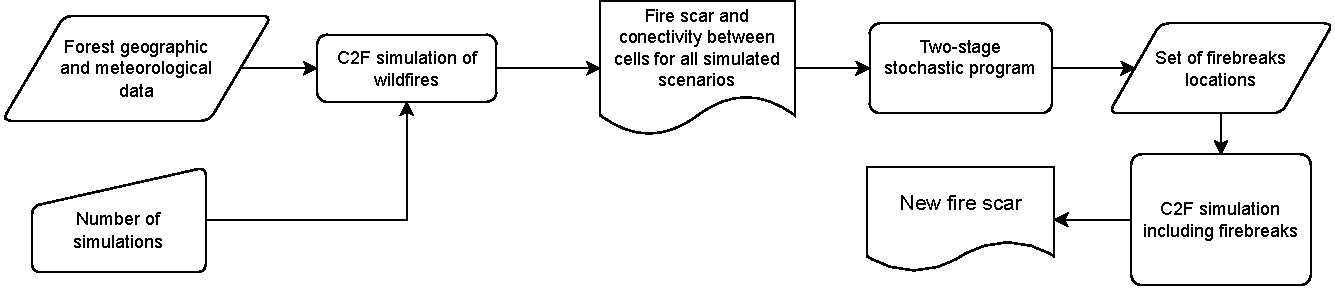
\includegraphics[width=1\textwidth]{figs/flowchart.pdf}
  \caption{Flowchart of the processes from C2F simulation of wildfires until the evaluation of solutions.}
  \label{fig:flowchart}
\end{figure}

\subsubsection{Static fire spread}

In order to assess the performance of the stochastic solution, we analyzed the expected percentage of burned area across all scenarios and the expected burned area for the $(1-\beta)$ scenarios where the burned area exceeds its Value-at-Risk. We recall that $\beta=0.9$ was considered for all instances. 

The relation between $\alpha$ and the expected burned area (resp. expected burned area for the $(1-\beta)$ scenarios) is presented in Fig.\:\ref{fig:validationA} (resp. Fig.\:\ref{fig:validationB}). The figures report the average value of five instances where the model was solved using 100 scenarios ($\texttt{FFP}(\vb{y}^*,\Omega, \lambda), \vert \mathcal{S} \rvert = 100$). The results suggest that increasing the number of firebreaks decreases the value of both measures. However, the marginal reduction is smaller as value $\alpha$ increases. For instance, when $\lambda = 1$, setting firebreak intensity to 0.01 reduces the average burned area of the forest by 4\%. In contrast, increasing $\alpha$ from 0.04 to 0.05 reduces the measurement by only 2\%. Similarly, for $\lambda = 0$ and $\lambda = 0.5$, the average of the 10\% worst-case scenario is reduced by 25\% when compared to simulations of forests without firebreaks concerning $\alpha = 0.01$. In contrast, when $\alpha$ is increased from 0.04 to 0.05, this value is reduced by only 8\%. This phenomenon can be attributed to the prioritization of firebreaks that are more effective at preventing fire spread. As $\alpha$ increases, each additional firebreak contributes less to reducing fire spread, which consequently results in a reduced impact on both studied metrics. 

On the other hand, in Fig.\:\ref{fig:validationB}, we see that the lower average percentage of the 10\% of worst cases was achieved using both $\lambda = 0.5$ and $\lambda = 0$. Consequently, considering that the expected burned area is lower using $\lambda = 0.5$ rather than $\lambda = 0$, the results suggest that minimizing a convex combination of the expected burned area and the CVaR risk measure is able to provide better results than only minimize the CVaR risk measure. It is important to note that for some instances with $\lambda = 0.5$ and $\lambda = 0$, optimality was not achieved. This explains why, for $\alpha = 0.03$ and $\alpha = 0.04$, the green curve is below the blue one.

\begin{figure}
%\centering
\begin{subfigure}[b]{0.5\linewidth}
    %\captionsetup{justification=centering}
    \centering
    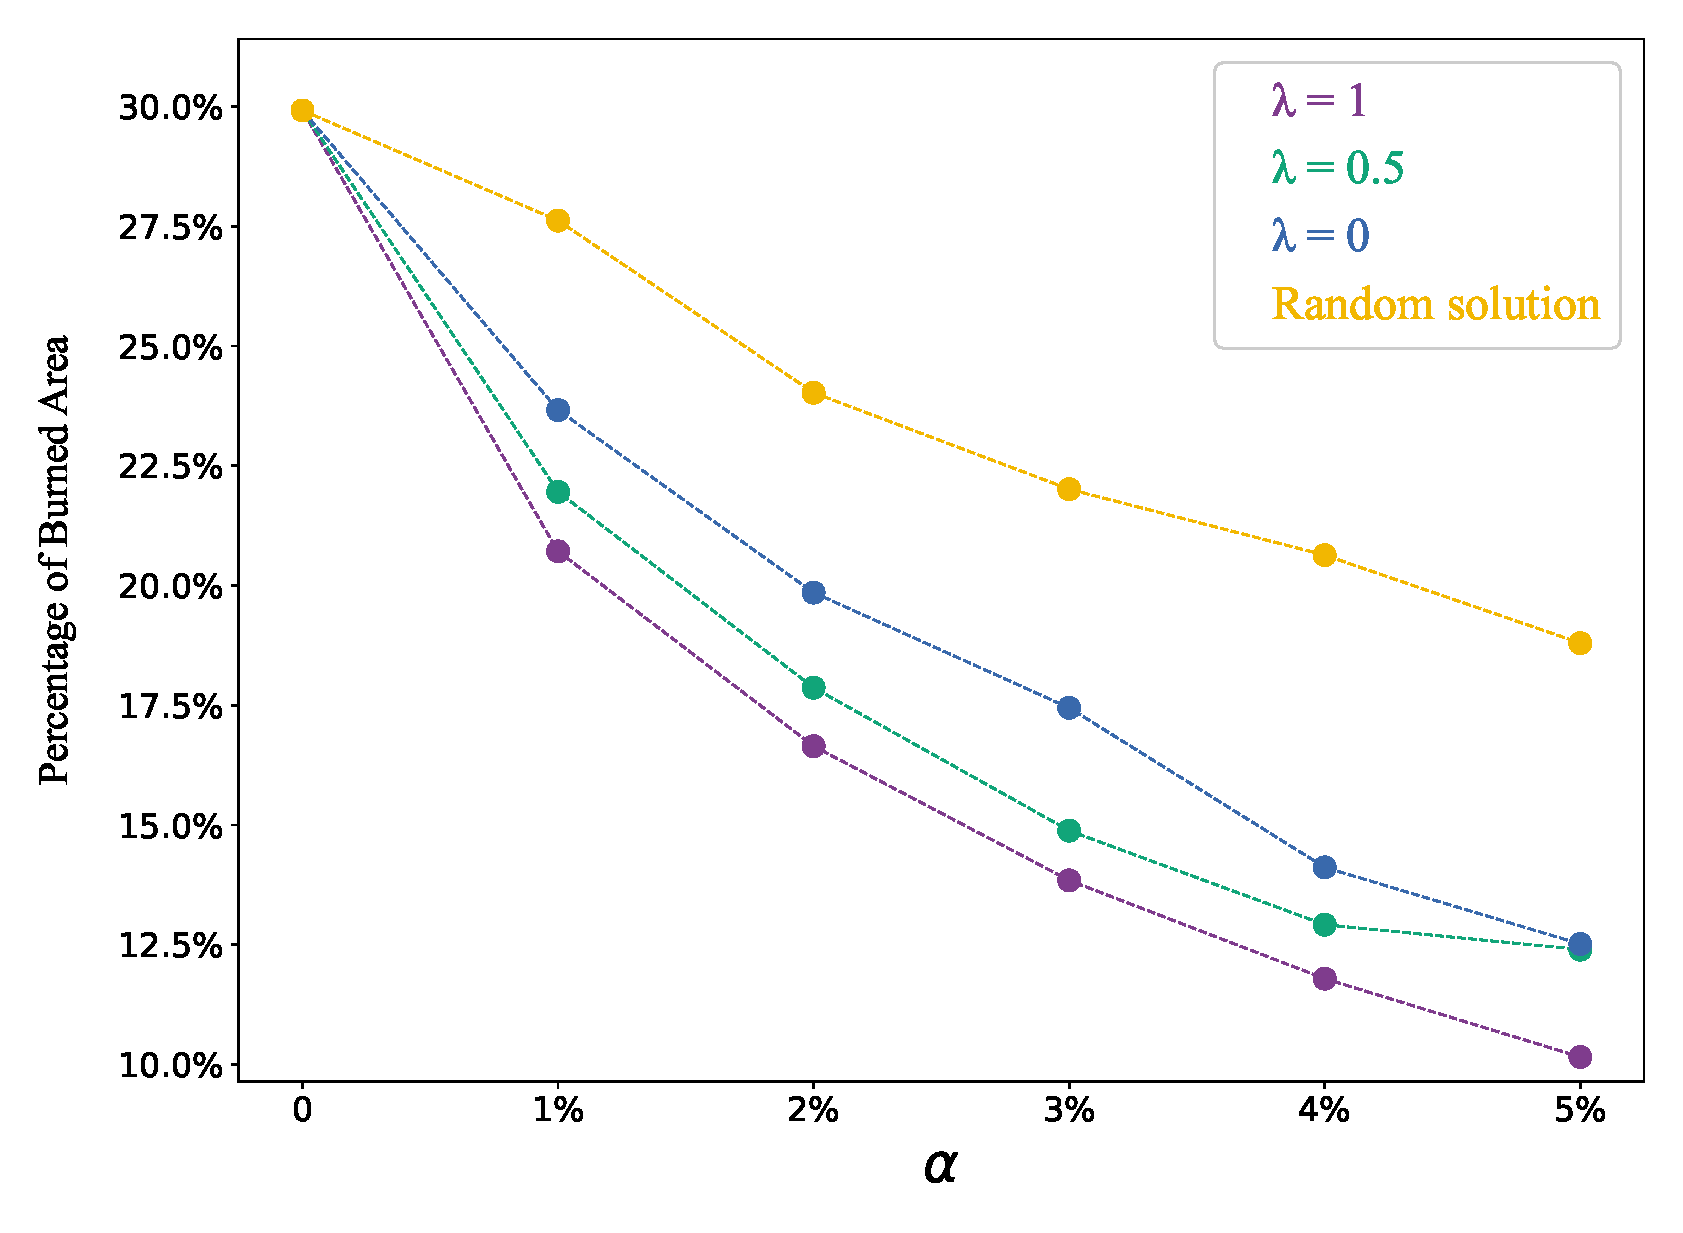
\includegraphics[width=0.9\linewidth]{figs/static100_1.eps}
    \caption{Percentage of burned area under different values of $\lambda$ }
    \label{fig:validationA}
    \vspace{1ex}
\end{subfigure}%%
\begin{subfigure}[b]{0.5\linewidth}
    %\captionsetup{justification=centering}
    \centering
    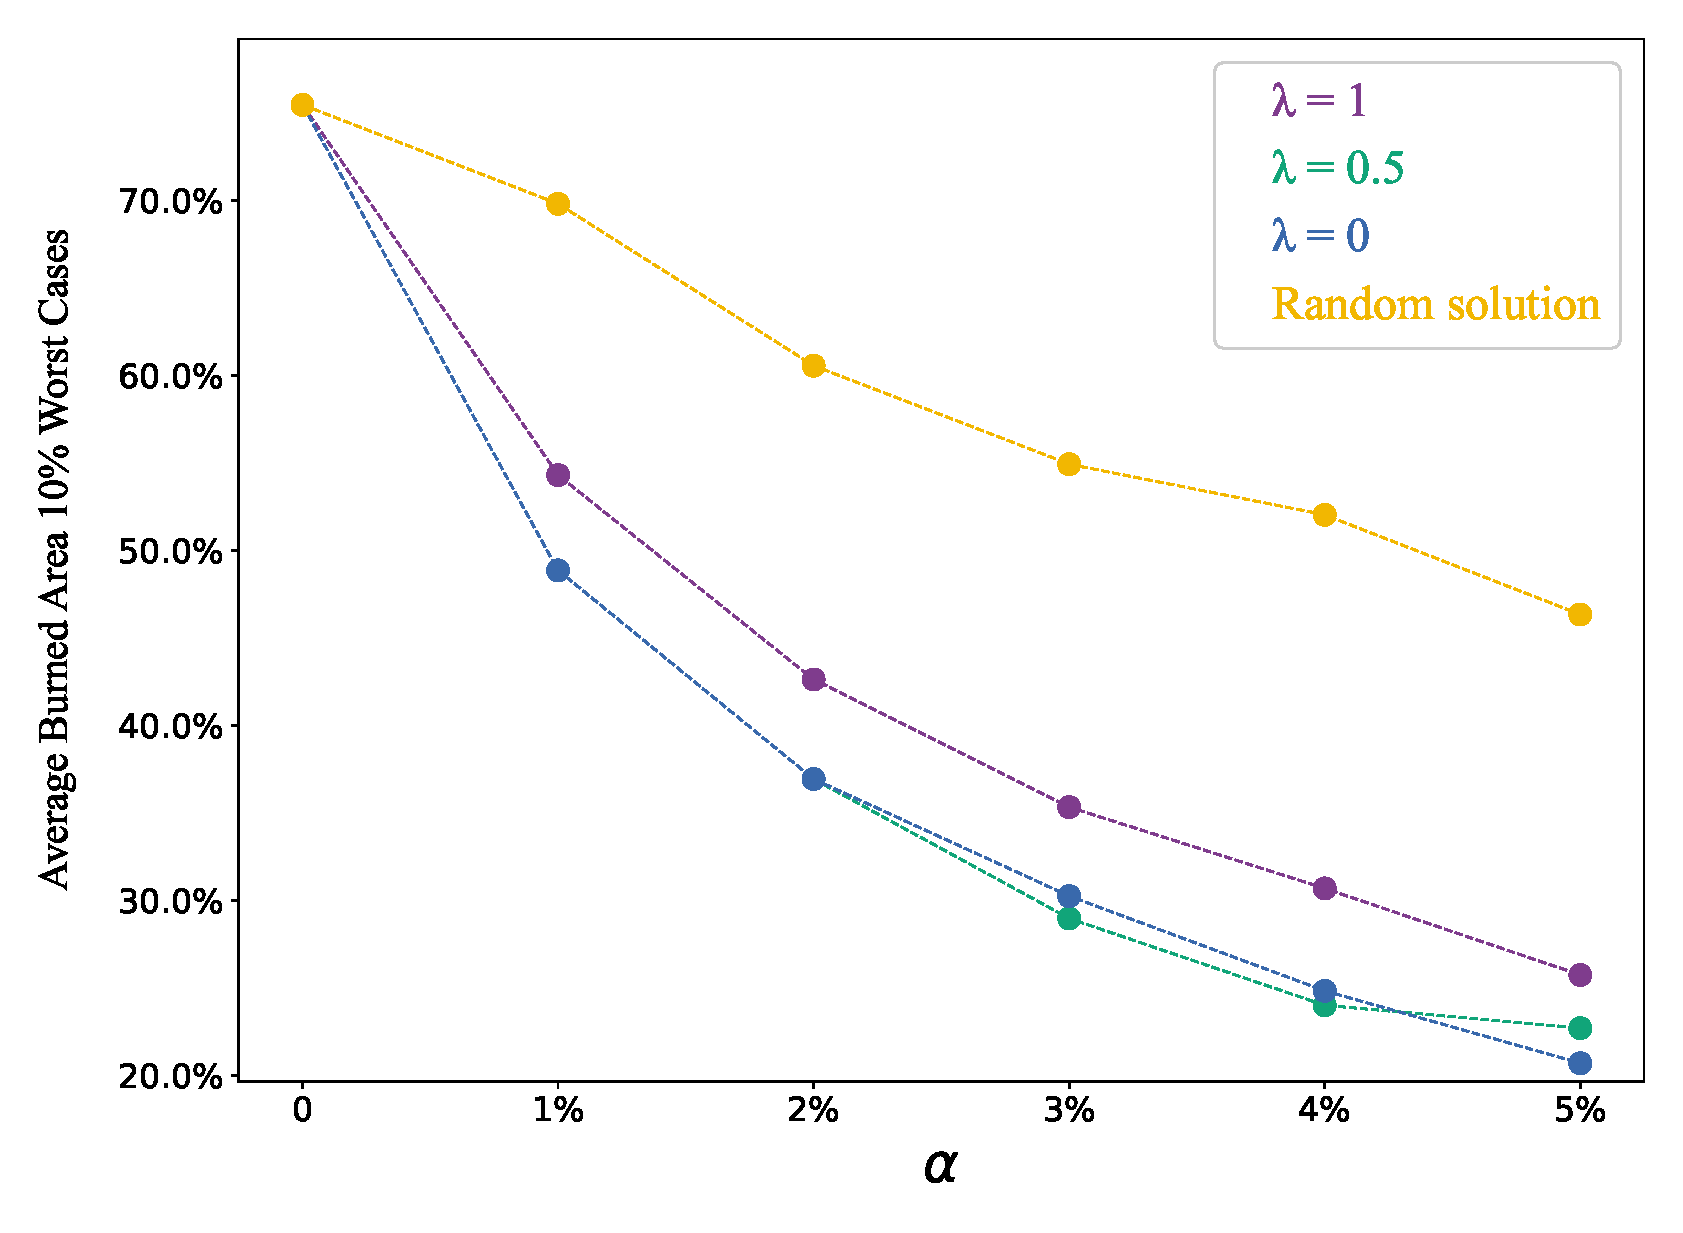
\includegraphics[width=0.9\linewidth]{figs/static100_2.eps}
    \caption{10\% worst-cases average under different values of $\lambda$}
    \label{fig:validationB}
    \vspace{1ex}
  \end{subfigure} 
\caption{Solutions provided by the model with $|\Omega|= 100$ scenarios}
\label{fig:validation}
\end{figure}

In both evaluations, we introduced a random solution that entered the program as the first-stage variables, so we only needed to capture the spread of fire resulting from that firebreak configuration. This random solution progressively added additional firebreaks for increasing values of $\alpha$ in order to not obtain worse results for greater percentage of land treated due to the randomness. The results indicate that this solution performs worse than all instances with different $\lambda$ and $\alpha$ values. In contrast with the random solution, $\lambda = 1$ achieves a reduction of almost 10\% in the burned area for all five instances. For $\lambda = 0$, it accomplishes a significant 30\% decrease in the average burned area for the 10\% of worst cases. This discrepancy arises due to the fact that the optimization model is capable of generating not only feasible solutions but also the optimal firebreak placement for the instances where the \texttt{MIP$_{gap}$} reaches zero.

Figure\:\ref{fig:static_1000} presents the results of the evaluation of the solutions obtained from the resolution of the instances described above into a test simulations set ($\texttt{FFP}(\vb{y}^{*},\mathcal{S}, \lambda), \lvert \mathcal{S} \rvert = 1,000$). The results show a better performance for $|\Omega| = 180$ and $|\Omega| = 100$ in both measures, for all values of $\lambda$ and $\alpha$. 

Furthermore, based on the findings, it can be observed that the solution derived from 20 scenarios outperforms the random solutions. However, when the value of $\alpha$ increases, the disparity between the two solutions decreases, resulting in the random solution being more favorable in certain instances (refer to Figure \ref{fig:static_1000} (b)). Simultaneously, the enhancement is further amplified when the number of scenarios is increased to 100 and 180. However, the incremental effect of raising the number of scenarios is diminished. Indeed, for $\lambda = 0.0$ and $\alpha \geq 0.04$, the solutions exhibit negligible differences. The aforementioned observation implies the importance of establishing an appropriate quantity of scenarios. Fewer scenarios may yield less competitive outcomes due to the presence of random solutions. Conversely, an excessively high number of scenarios may not result in a substantial enhancement and unnecessarily inflate computational demand. This suggests the presence of a trade-off between the quality of the solution and the processing time required.

If we compare this to the results presented in Fig.\:\ref{fig:validation}, it is possible to observe a decrease in the effectiveness of the firebreaks, but achieving an important reduction in the percentage of burned area and average burned area for the 10\% of worst cases. This suggests that the sampling of scenarios is efficient and that the solutions are robust enough to perform well when evaluated on a much larger set of scenarios.



\begin{figure}[h!]
\centering
\begin{subfigure}[b]{0.5\linewidth}
    \centering
    %\captionsetup{justification=centering}
    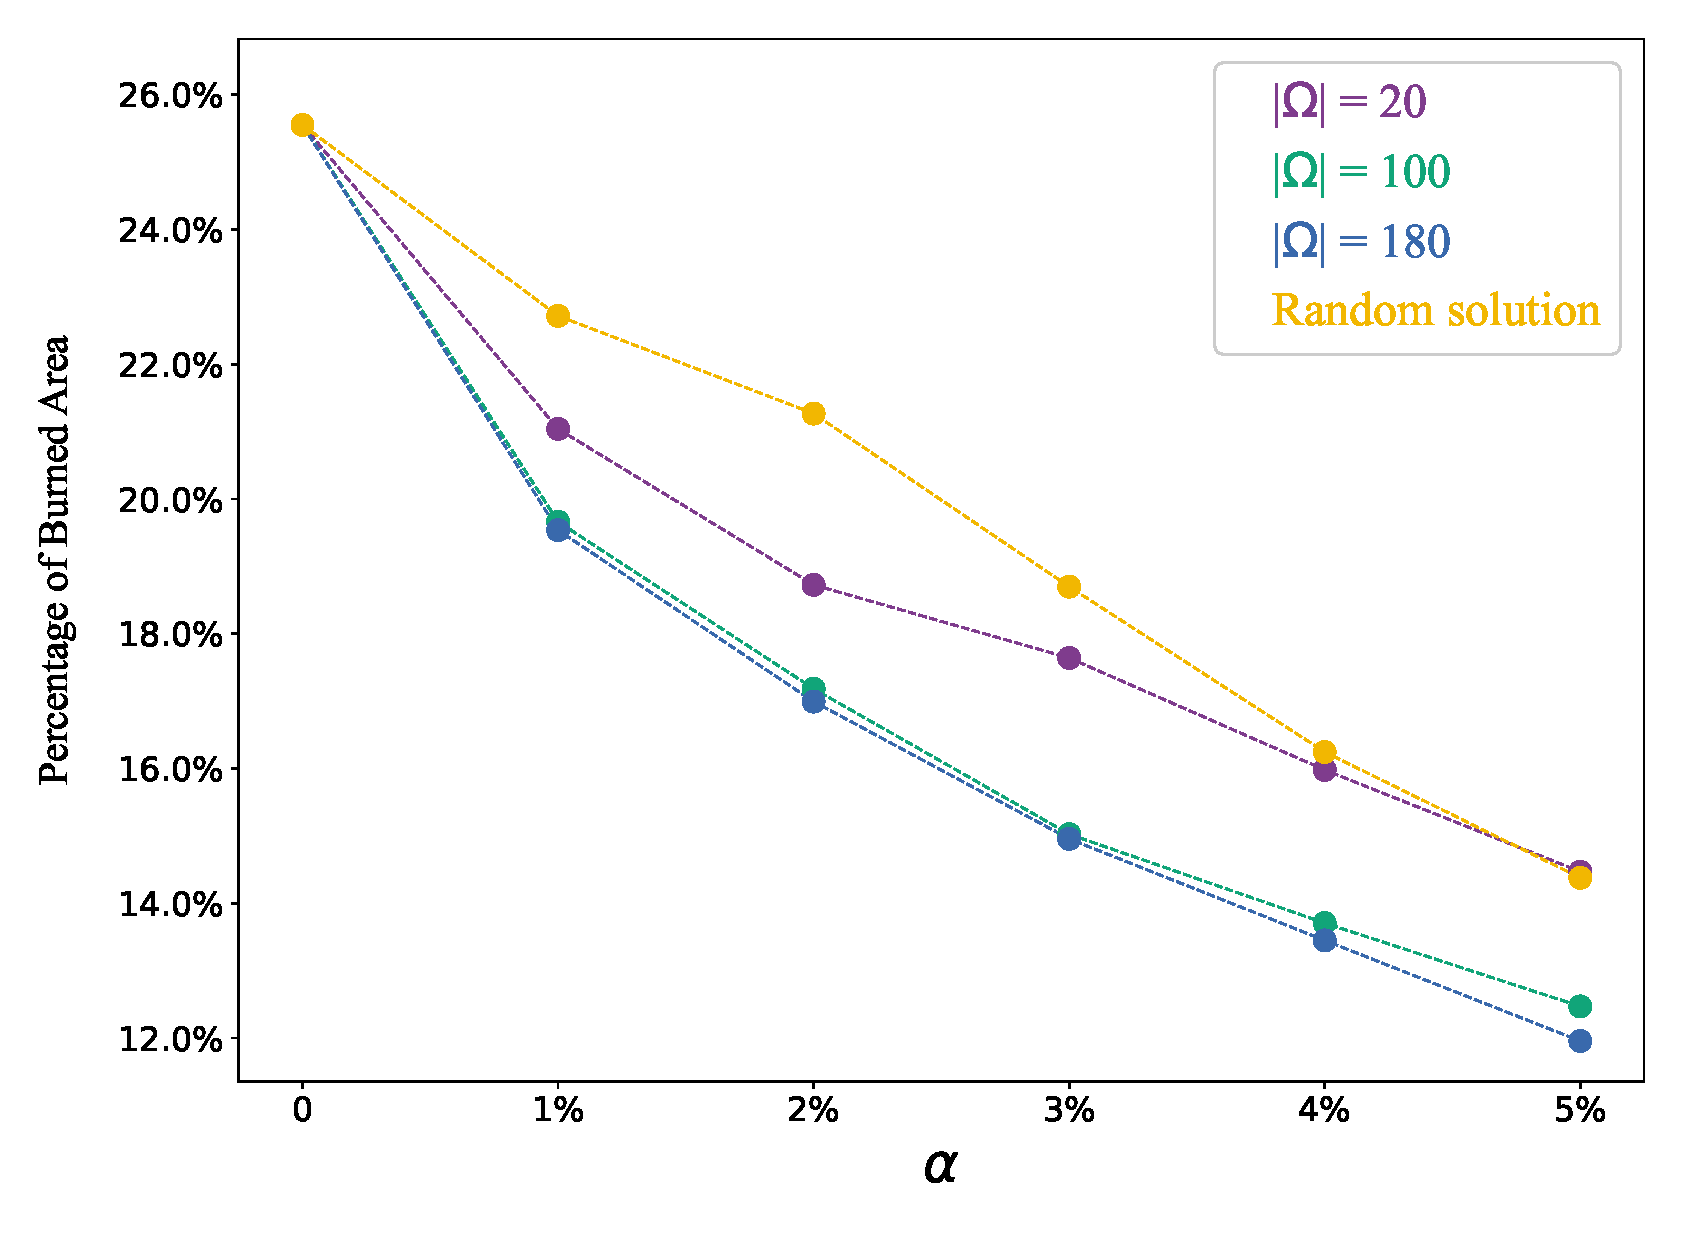
\includegraphics[width=0.9\linewidth]{figs/static1000_1.eps}
    \caption{Average burned area by $|\Omega|$ for $\lambda = 1.0$.}
    %\vspace{1ex}
\end{subfigure}%%
\begin{subfigure}[b]{0.5\linewidth}
    \centering
    %\captionsetup{justification=centering}
    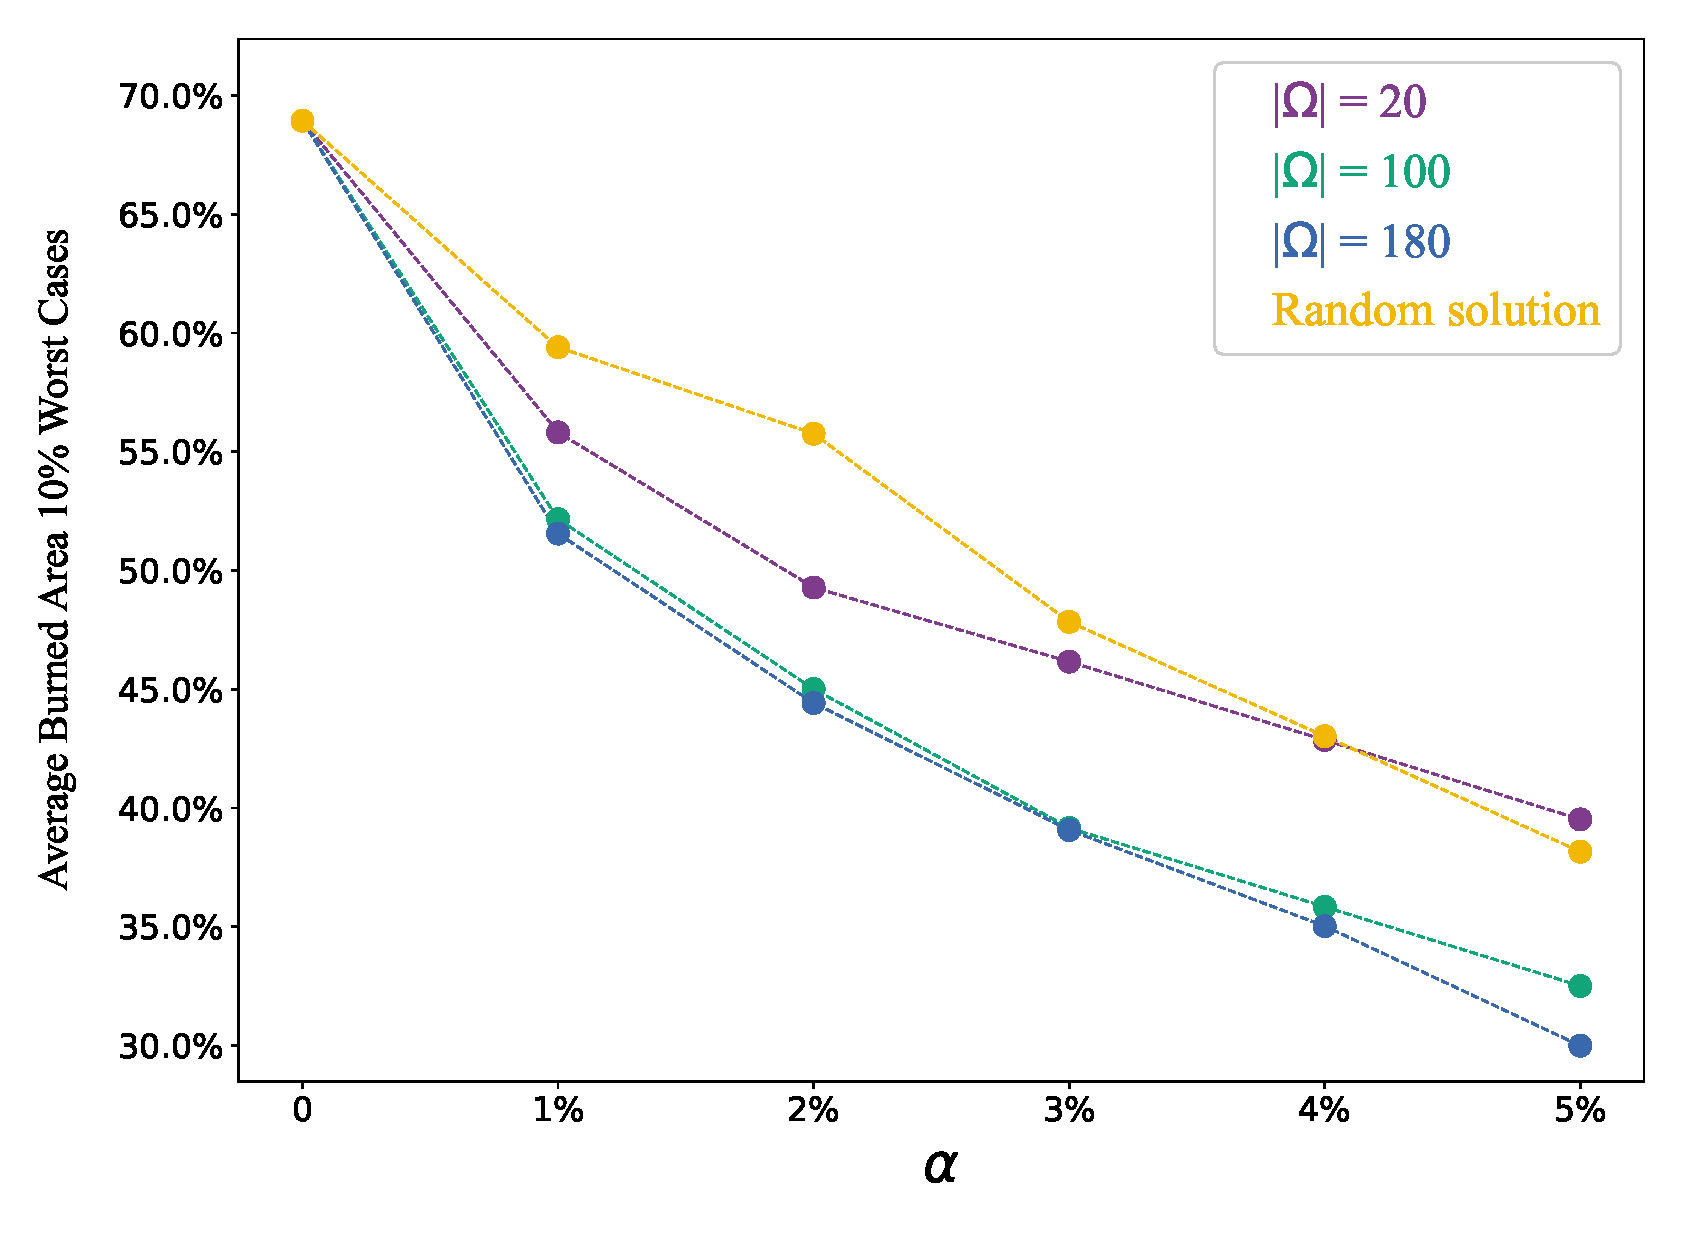
\includegraphics[width=0.9\linewidth]{figs/static1000_2.eps}
    \caption{10\% worst case average by $|\Omega|$ for $\lambda = 1.0$}
    %\vspace{1ex}
  \end{subfigure} 
\begin{subfigure}[b]{0.5\linewidth}
    \centering
    %\captionsetup{justification=centering}
    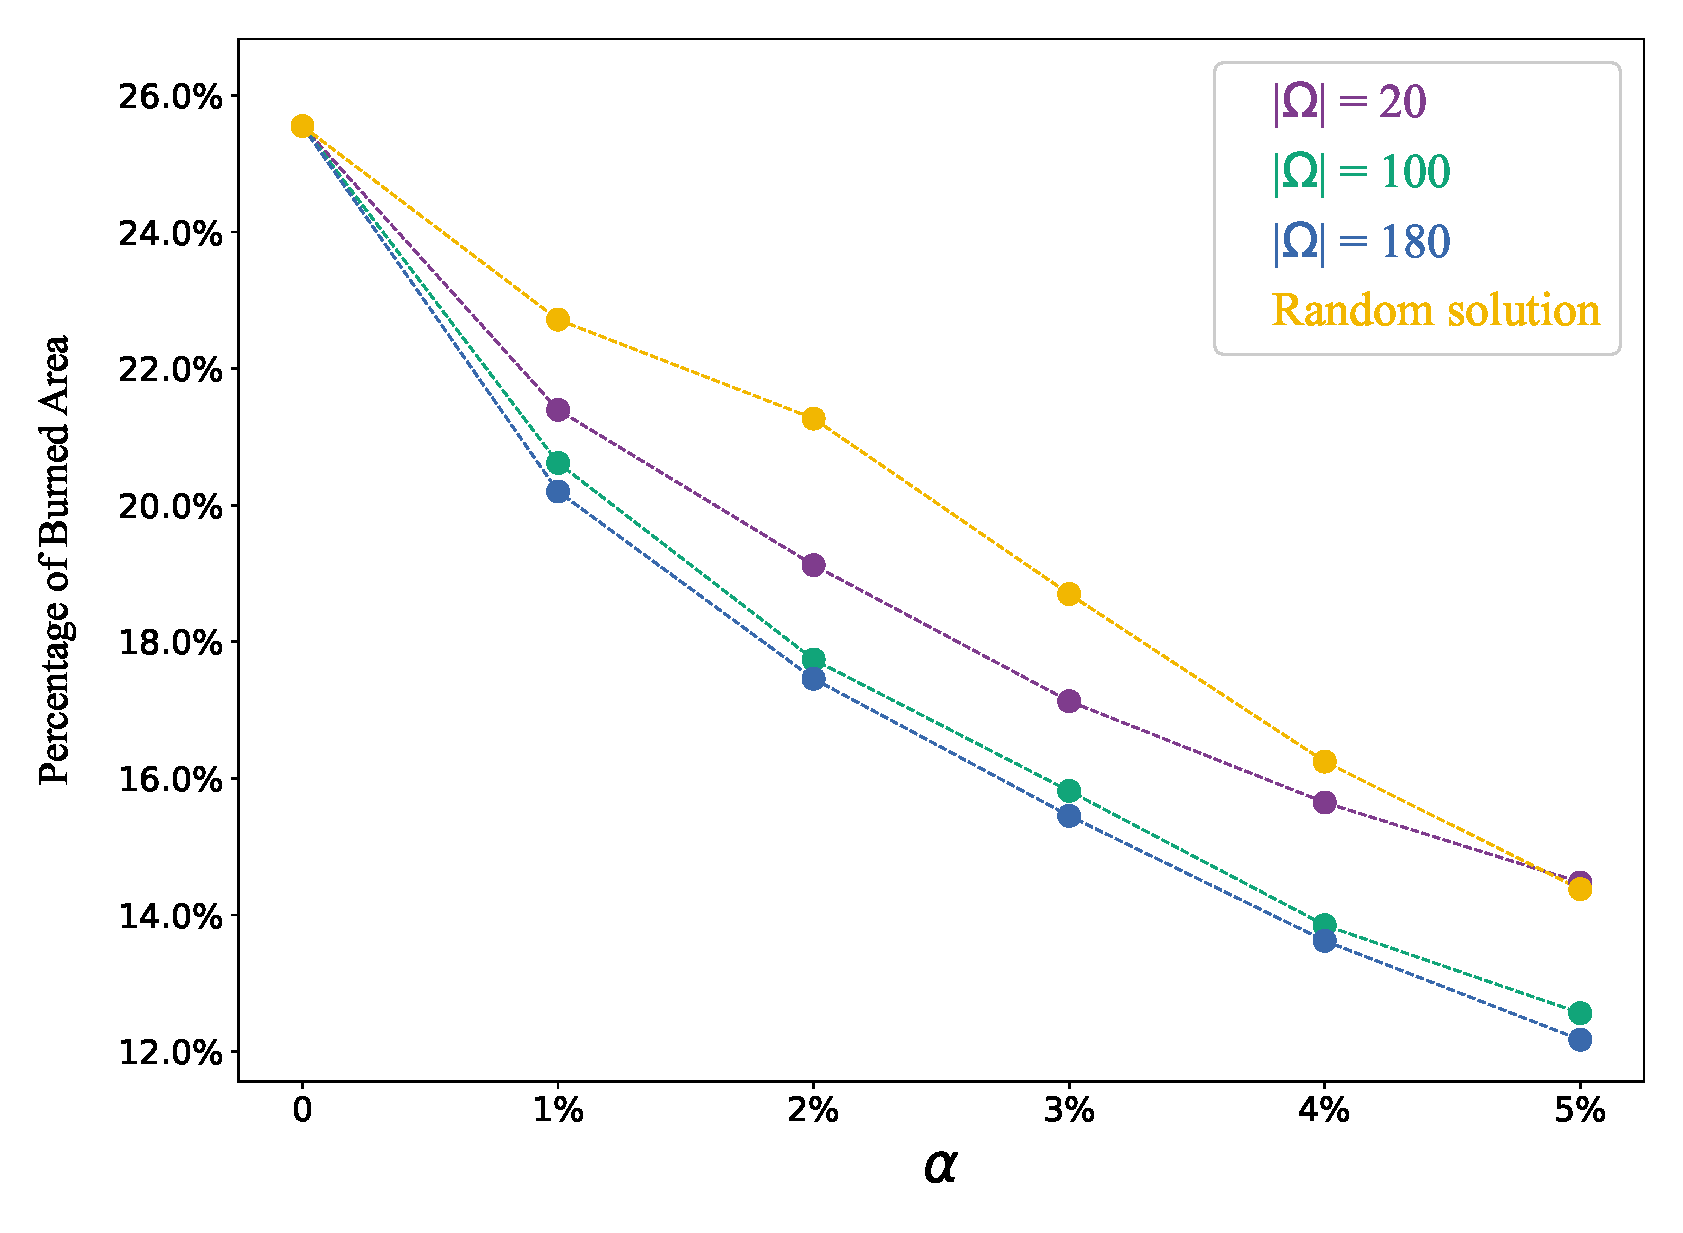
\includegraphics[width=0.9\linewidth]{figs/static1000_3.eps}
    \caption{Average burned area by $|\Omega|t$ for $\lambda = 0.5$.}
%    \vspace{1ex}
  \end{subfigure}%% 
\begin{subfigure}[b]{0.5\linewidth}
    \centering
    %\captionsetup{justification=centering}
    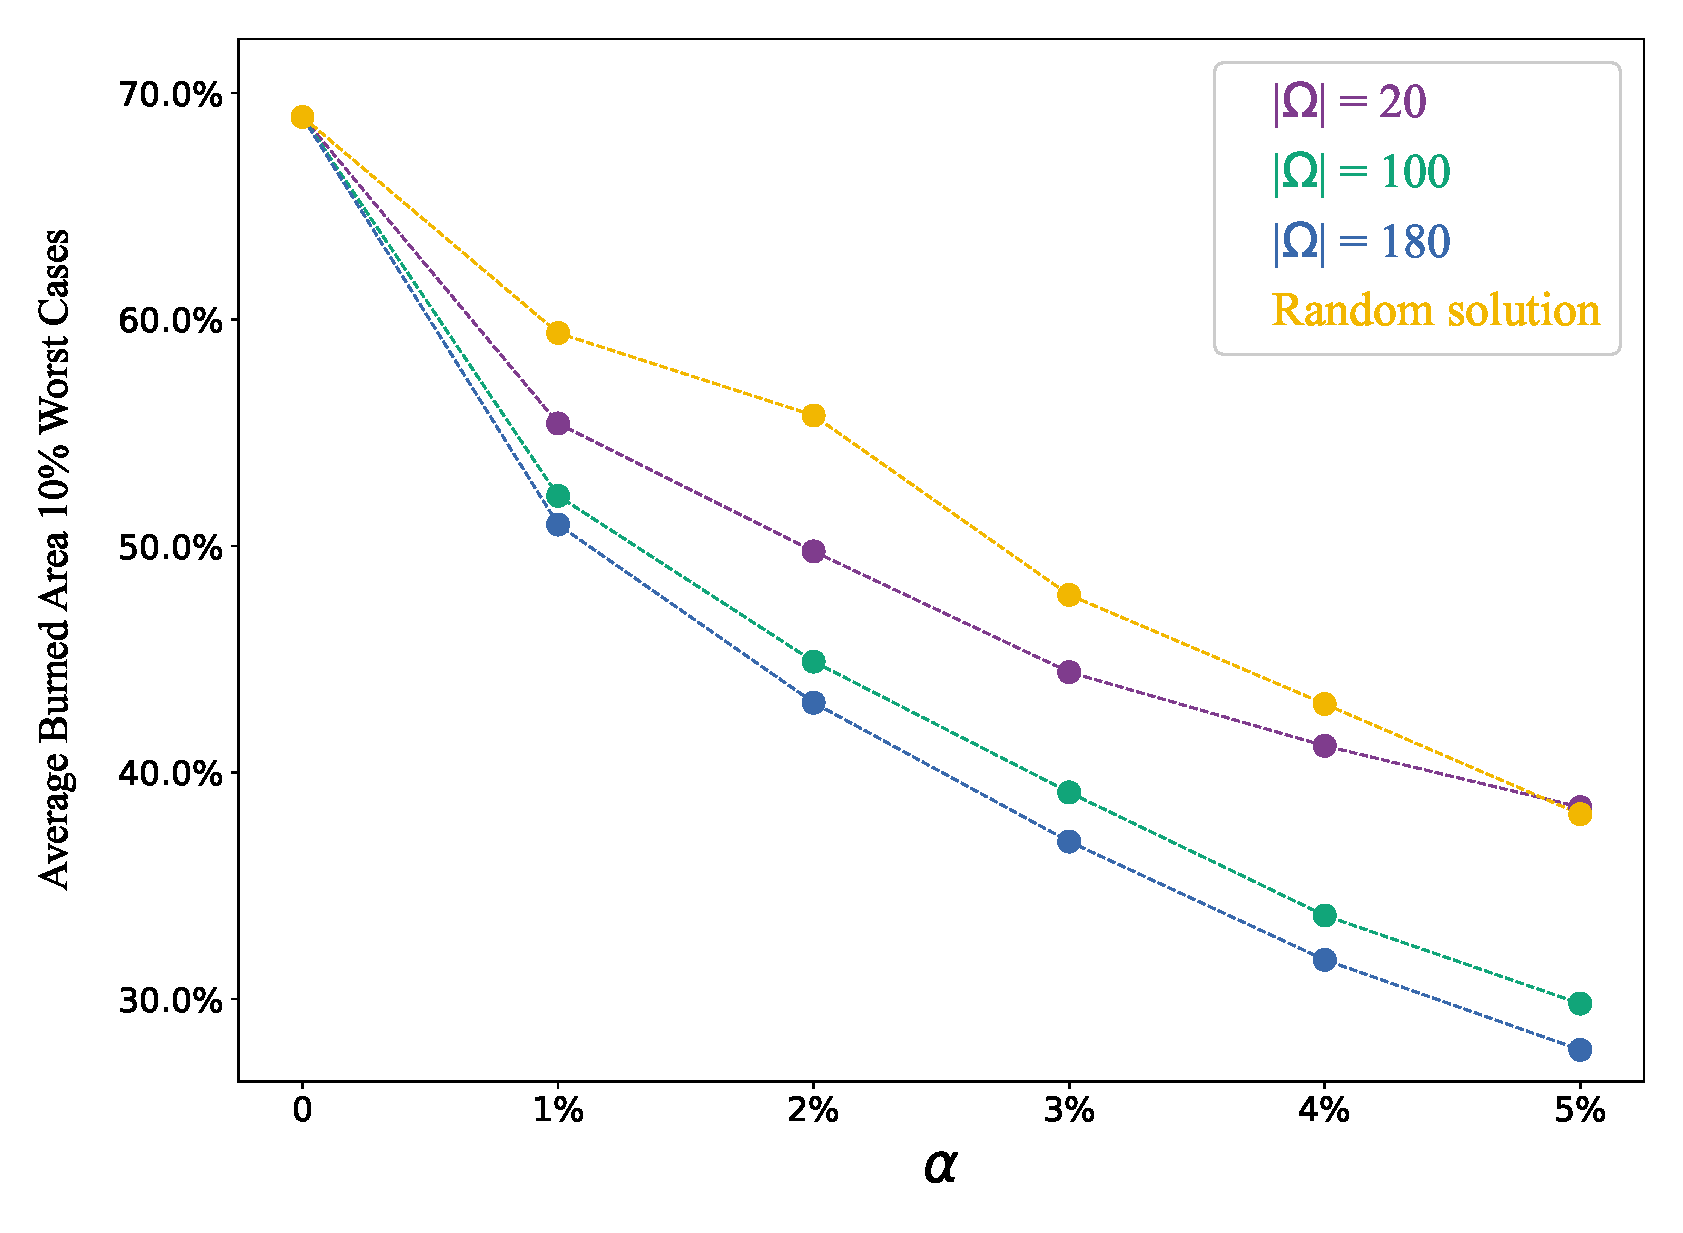
\includegraphics[width=0.9\linewidth]{figs/static1000_4.eps}
    \caption{10\% worst case average by $|\Omega|$ for $\lambda = 0.5$.}
    %\vspace{1ex}
  \end{subfigure} 
\begin{subfigure}[b]{0.5\linewidth}
    \centering
    %\captionsetup{justification=centering}
    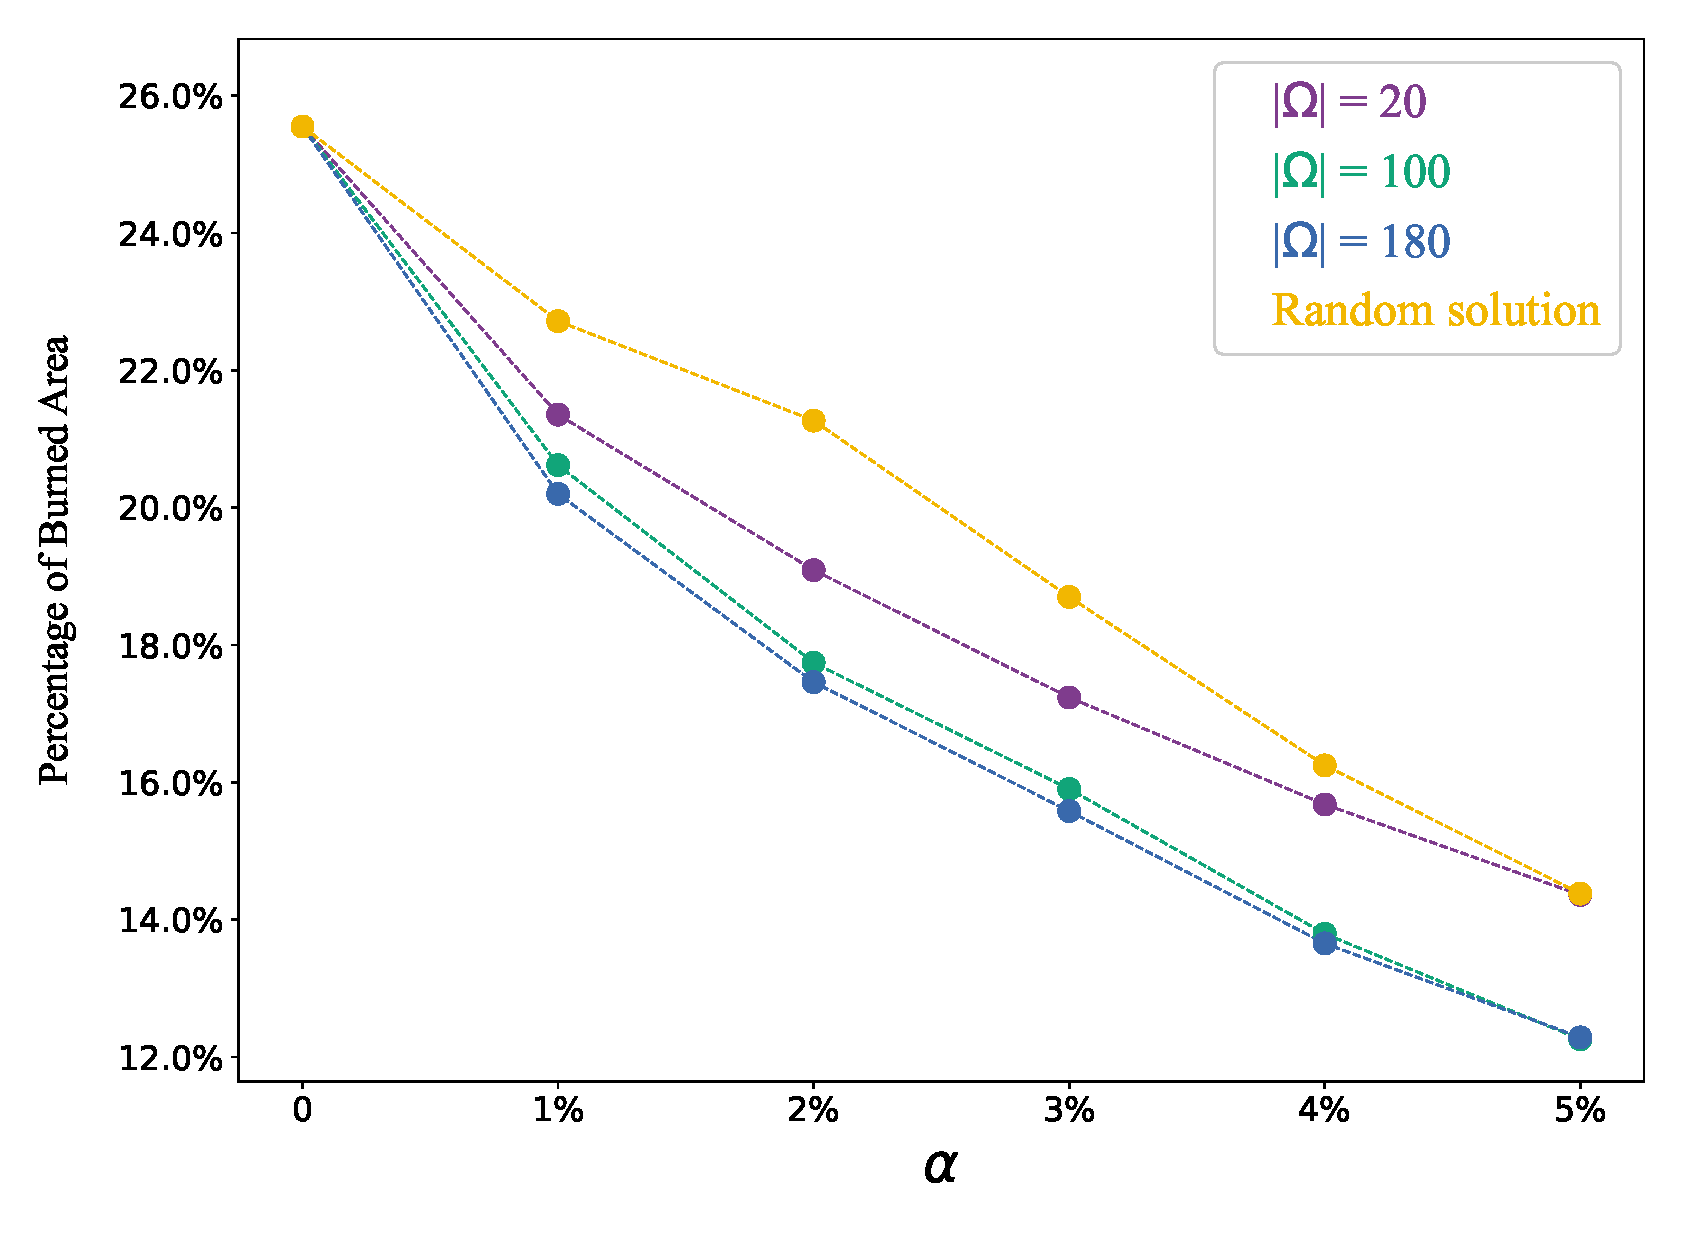
\includegraphics[width=0.9\linewidth]{figs/static1000_5.eps}
    \caption{Average burned area by $|\Omega|$ for $\lambda = 0.0$.}
%    \vspace{1ex}
  \end{subfigure}%% 
\begin{subfigure}[b]{0.5\linewidth}
    \centering
    %\captionsetup{justification=centering}
    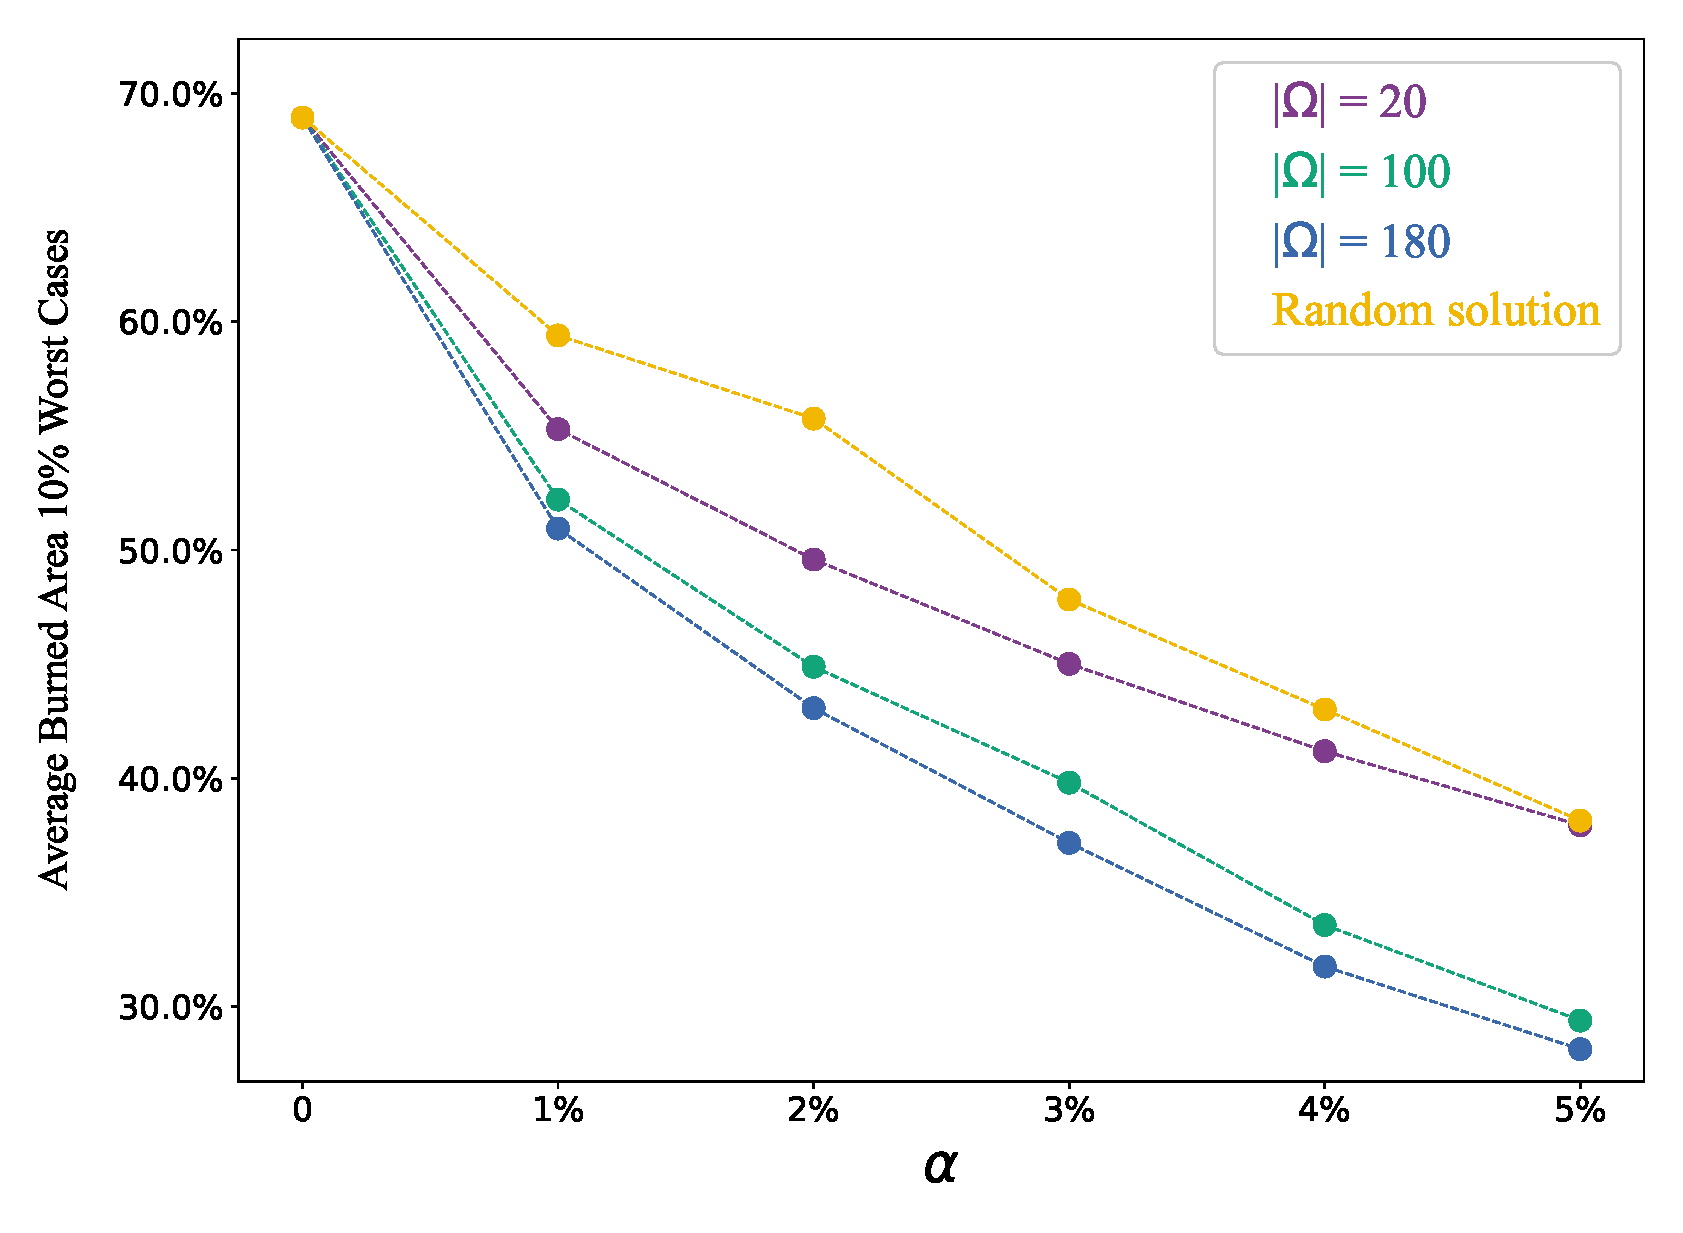
\includegraphics[width=0.9\linewidth]{figs/static1000_6.eps}
    \caption{10\% worst case average by $|\Omega|$ for $\lambda = 0.0$}
    %\vspace{1ex}
  \end{subfigure} 
\caption{Evaluation of the solutions on 1,000 scenarios, considering static fire, $|\Omega|$ size assessment.}
\label{fig:static_1000}
\end{figure}

Figures\:\ref{fig:solutions_l1} and \ref{fig:solutions_l05} displays the spatial arrangement of solutions using $\alpha$ = 0\%(A), 1\%(B), 3\%(C), and 5\%(D), and $\lambda = 1.0$ and $\lambda = 0.5$, respectively. As the number of harvested cells increases, a clear reduction in burned areas can be observed. However, no easily identifiable pattern emerges when examining the spatial distribution of firebreaks, although some barriers form between $\alpha$ levels of 3\% and 5\%. These results support the findings presented in \citep{finney2007simulation}, which indicate that the selection of locations changes as $\alpha$ varies. Some firebreak placements chosen at 1\% were not selected at 3\%, and some of those chosen at 3\% were not selected at 5\%, suggesting that the solutions are not a simple iterative process of aggregating harvested cells but rather a more complex selection process. Simultaneously, the configuration of firebreaks undergoes alterations based on the $\lambda$ parameter, resulting in modifications to the areas being protected. It is worth mentioning that the solution provided by different value of $\lambda$ also differ between them, the firebreaks placed at $\lambda = 0.5$ tends to be more contiguous, separating the land into zones and preventing the formation of large wildfires.

\begin{figure}[h!]
\centering
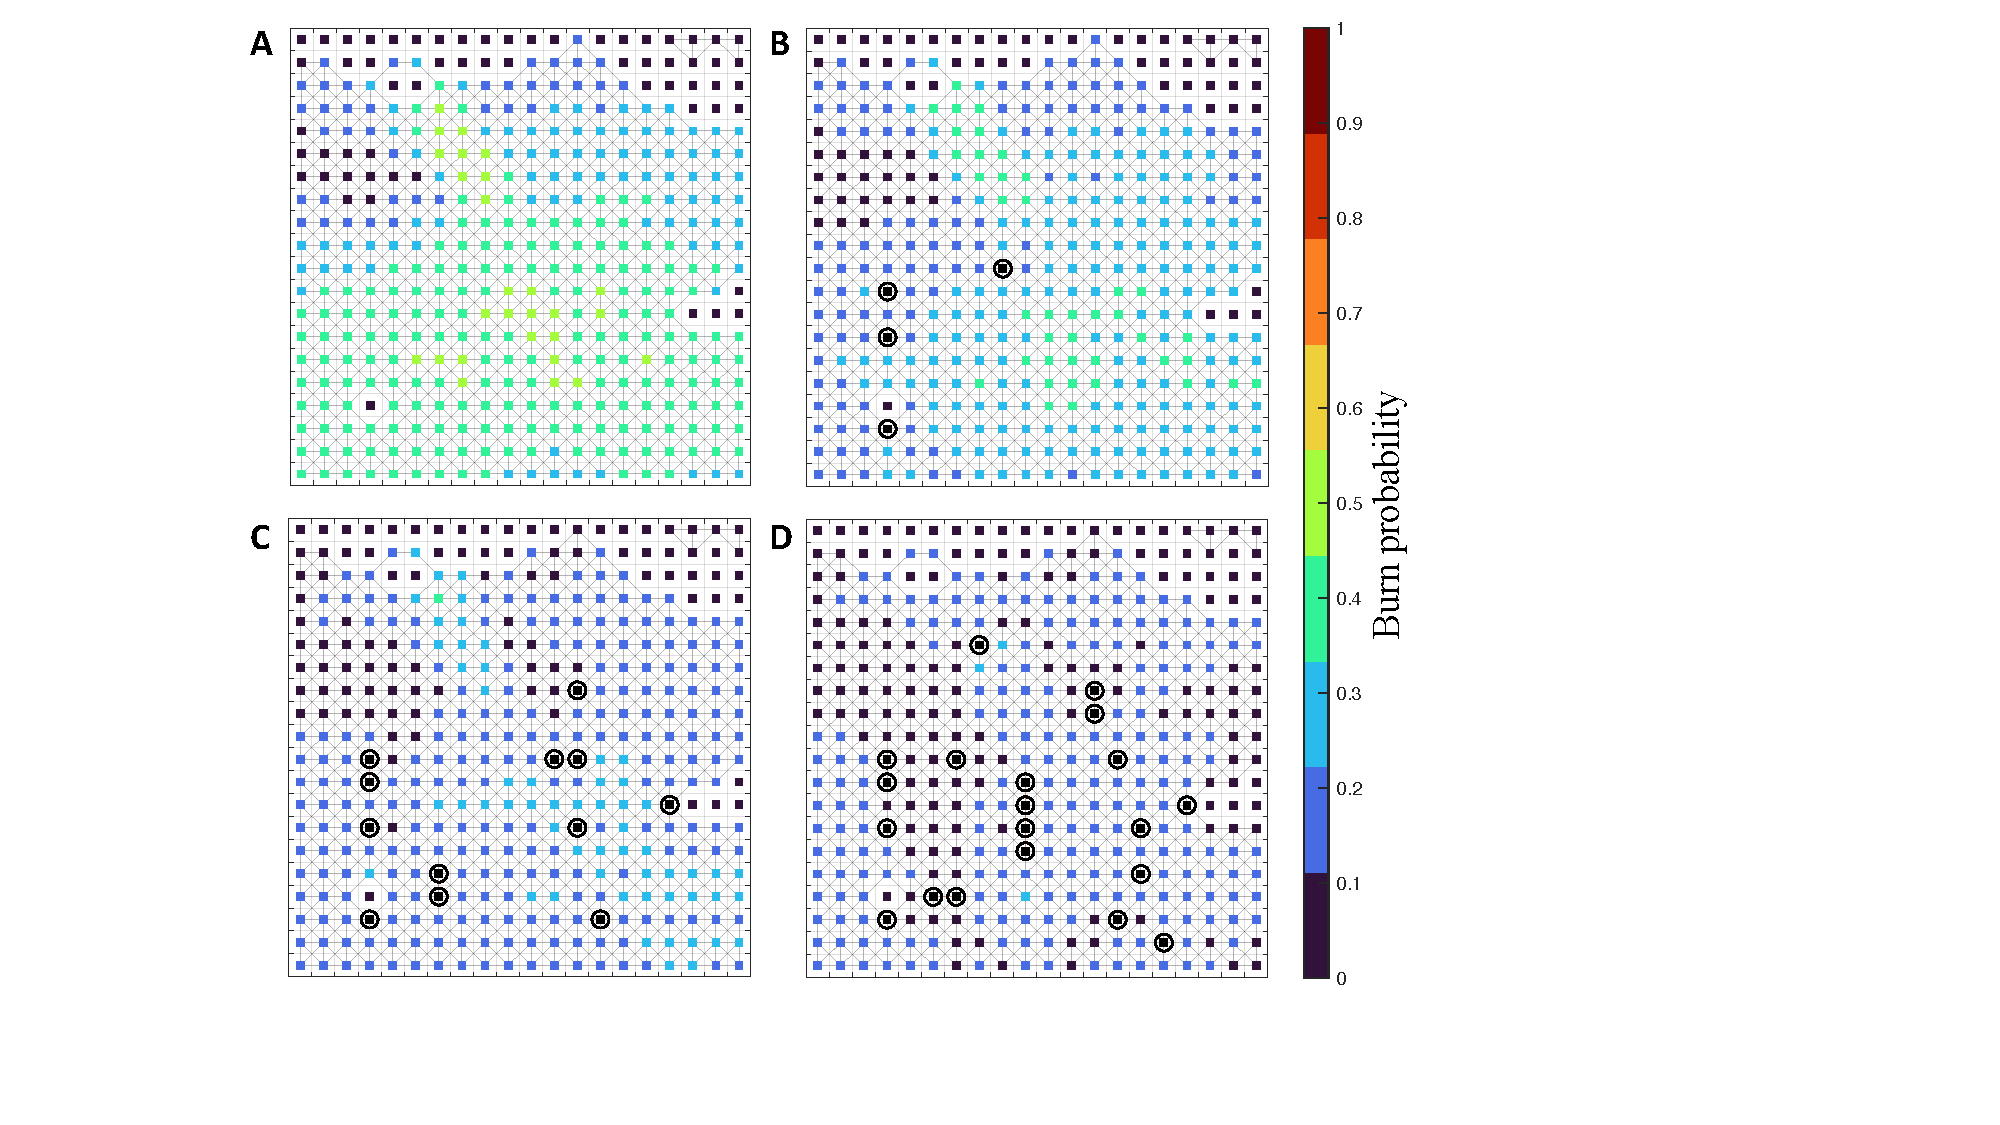
\includegraphics[scale=0.7]{figs/solutions_lb1.pdf}
\caption{Firebreak placement for the solution of the forest \texttt{Sub20}, using $|\Omega| = 100$ and $\lambda = 1$. $\alpha$ varies from 0\% (A) to 5\% (D). Firebreaks are depicted in black circles.}
\label{fig:solutions_l1}
\end{figure}

\begin{figure}[h!]
\centering
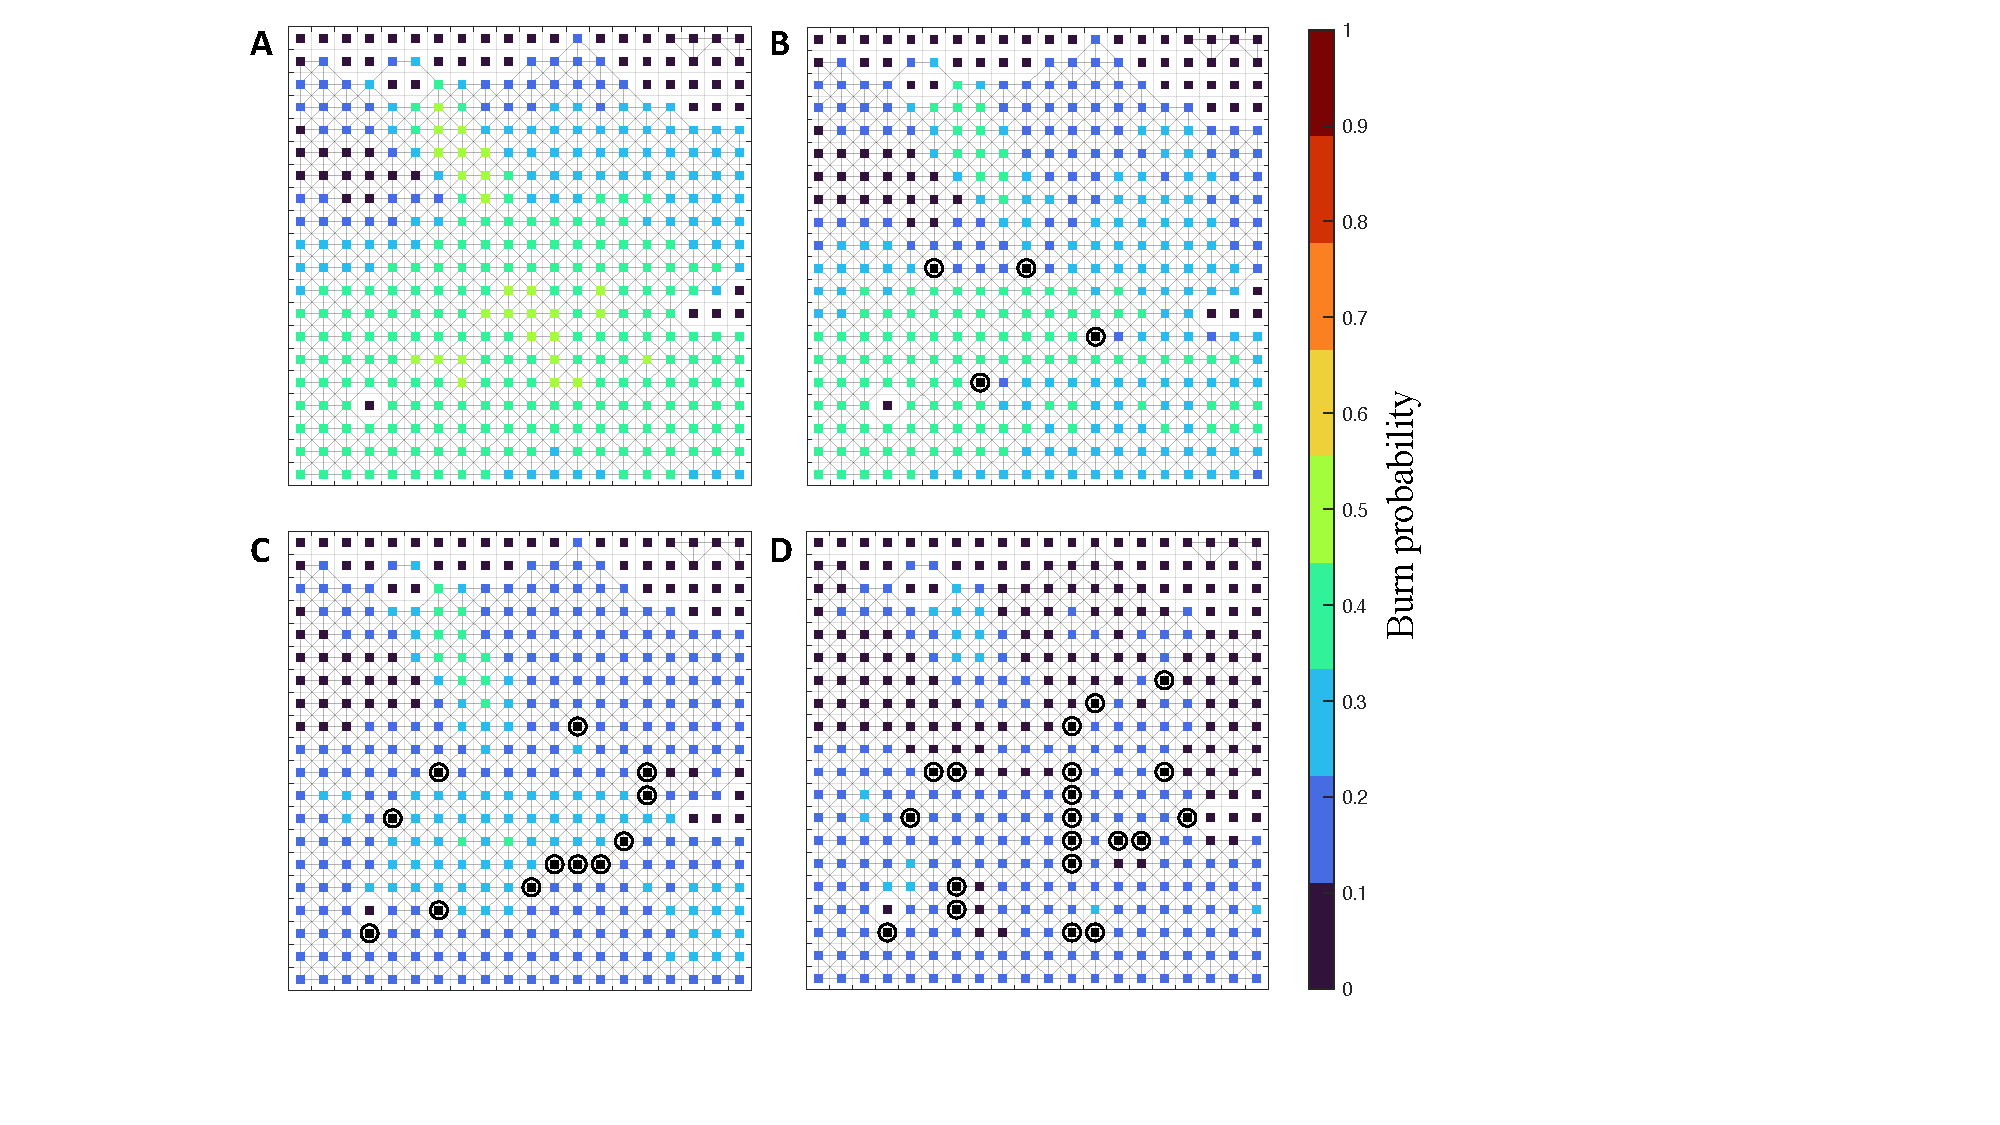
\includegraphics[scale=0.7]{figs/solutions_lb05.pdf}
\caption{Firebreak placement for the solution of the forest \texttt{Sub20}, using $|\Omega| = 100$ and $\lambda = 0.5$. $\alpha$ varies from 0\% (A) to 5\% (D). Firebreaks are depicted in black circles.}
\label{fig:solutions_l05}
\end{figure}

\subsubsection{Dynamic fire spread}

\begin{figure}[h!]
\centering
\begin{subfigure}[b]{0.5\linewidth}
    \centering
    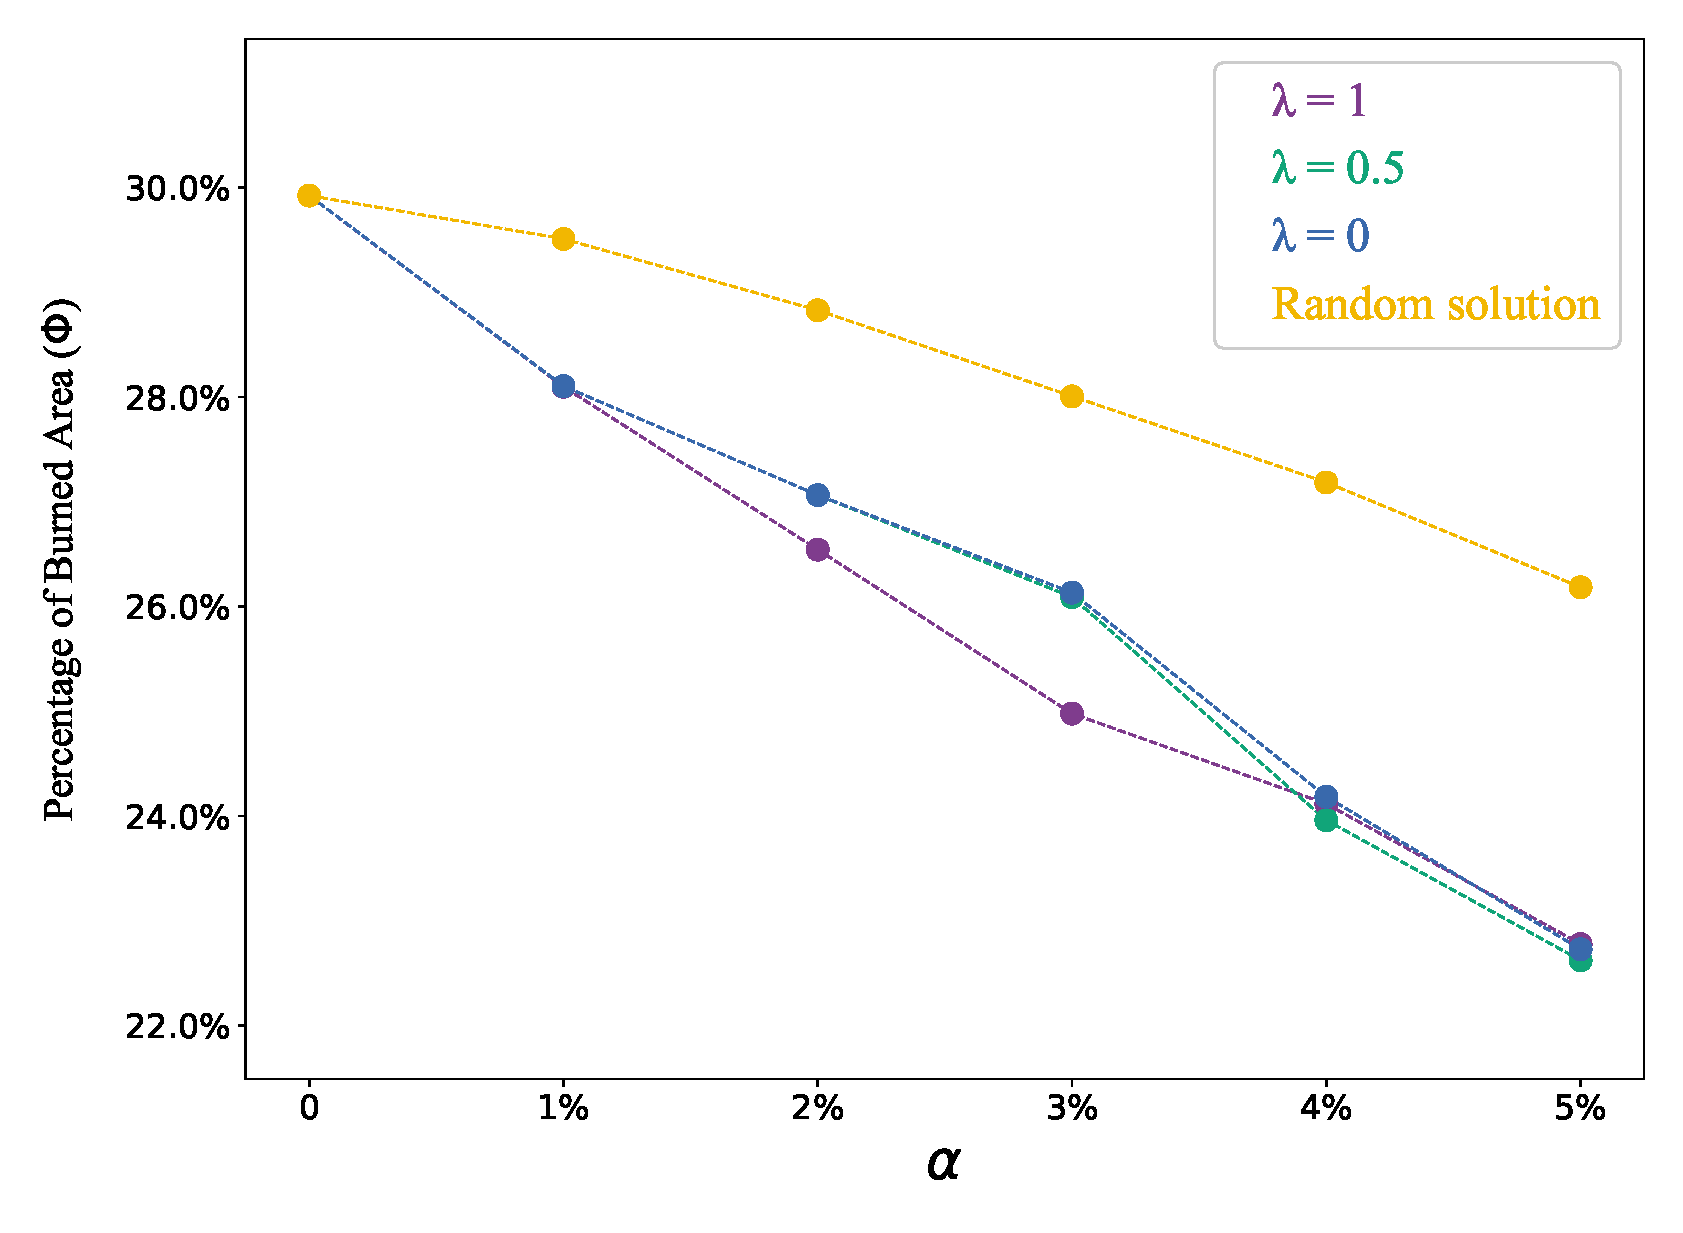
\includegraphics[width=0.9\linewidth]{figs/dinamic100_1.eps}
    \caption{Percentage of burned area under different values of $\lambda$ }
    \label{fig:validation2A}
    \vspace{1ex}
\end{subfigure}%%
\begin{subfigure}[b]{0.5\linewidth}
    %\centering
    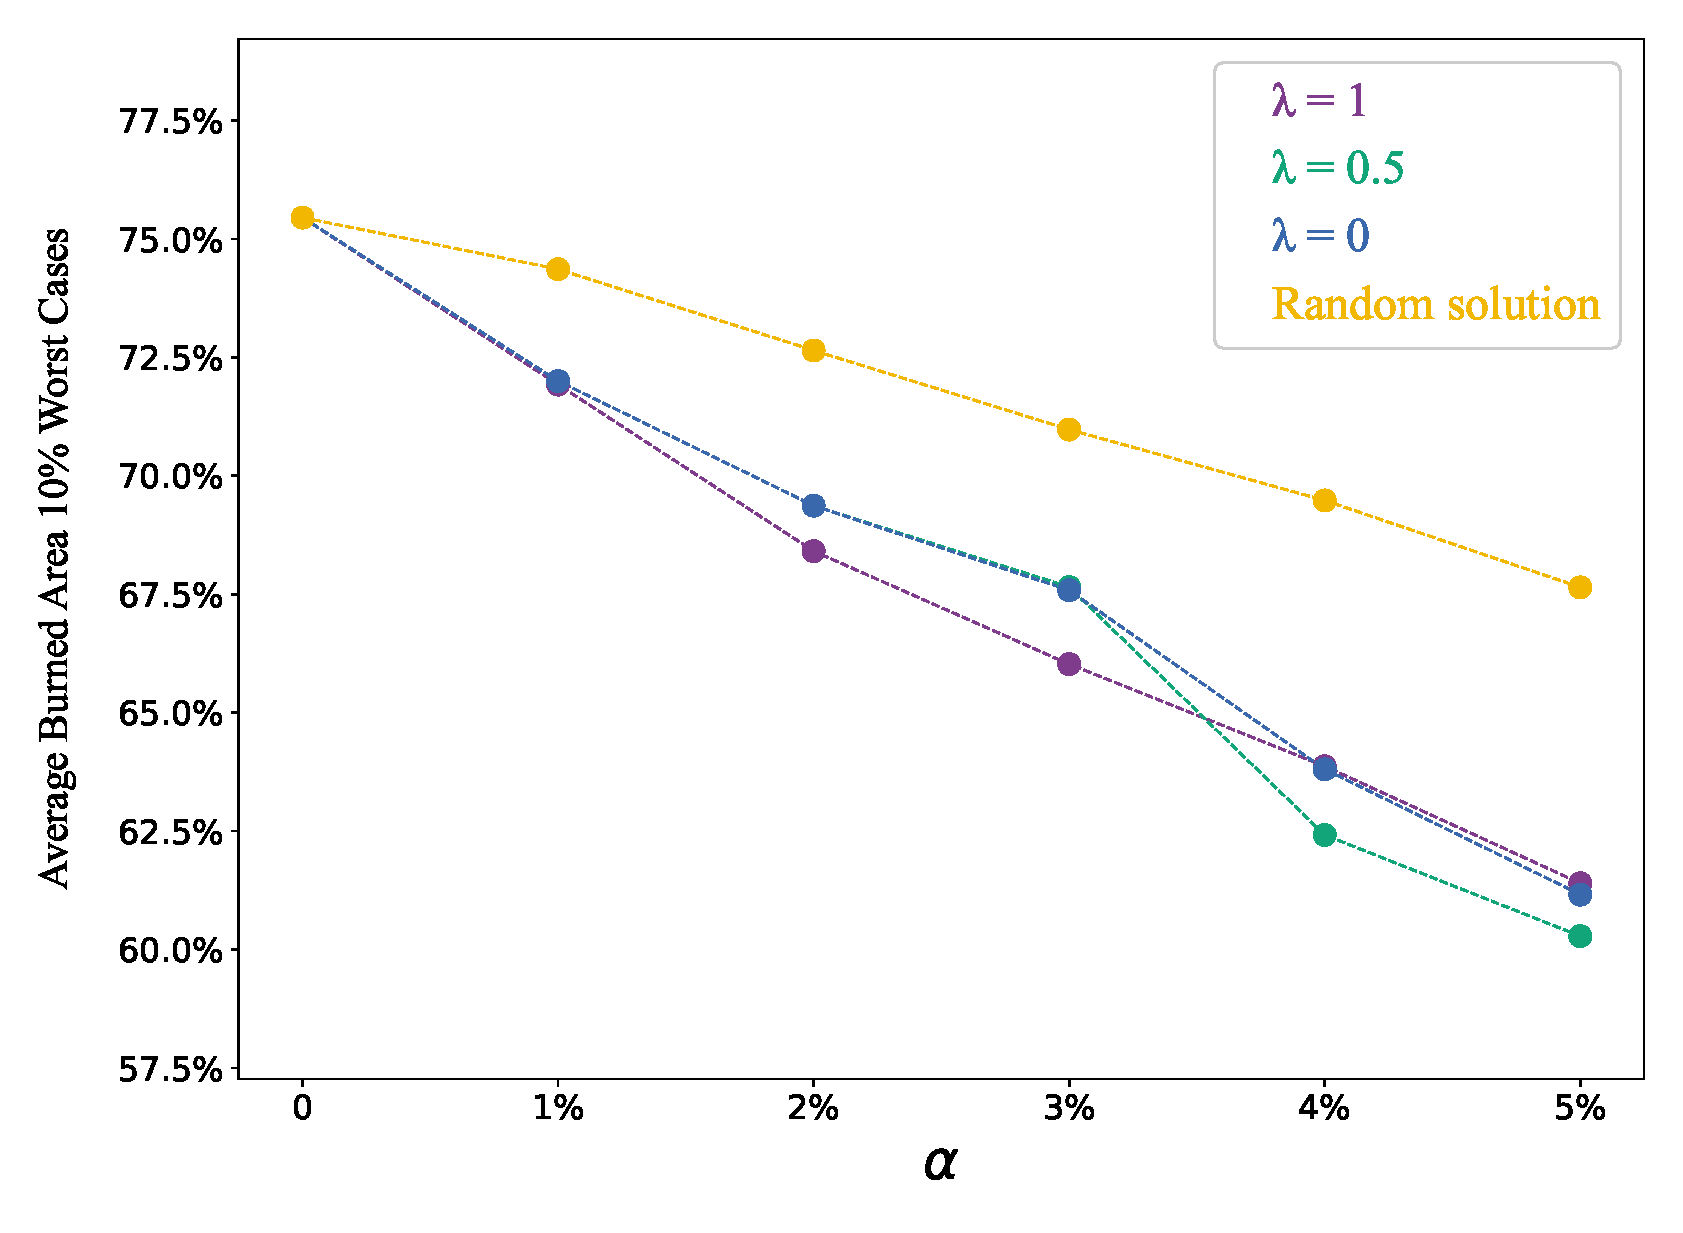
\includegraphics[width=0.9\linewidth]{figs/dinamic100_2.eps}
    \caption{10\% worst-cases average under different values of $\lambda$}
    \label{fig:validation2B}
    \vspace{1ex}
  \end{subfigure} 
\caption{Evaluation of the solutions using C2F on set $\Omega$ used for solving the model.}
\label{fig:evaluation1}
\end{figure} 

\begin{figure}[h!]
\centering
\begin{subfigure}[b]{0.5\linewidth}
    \centering
    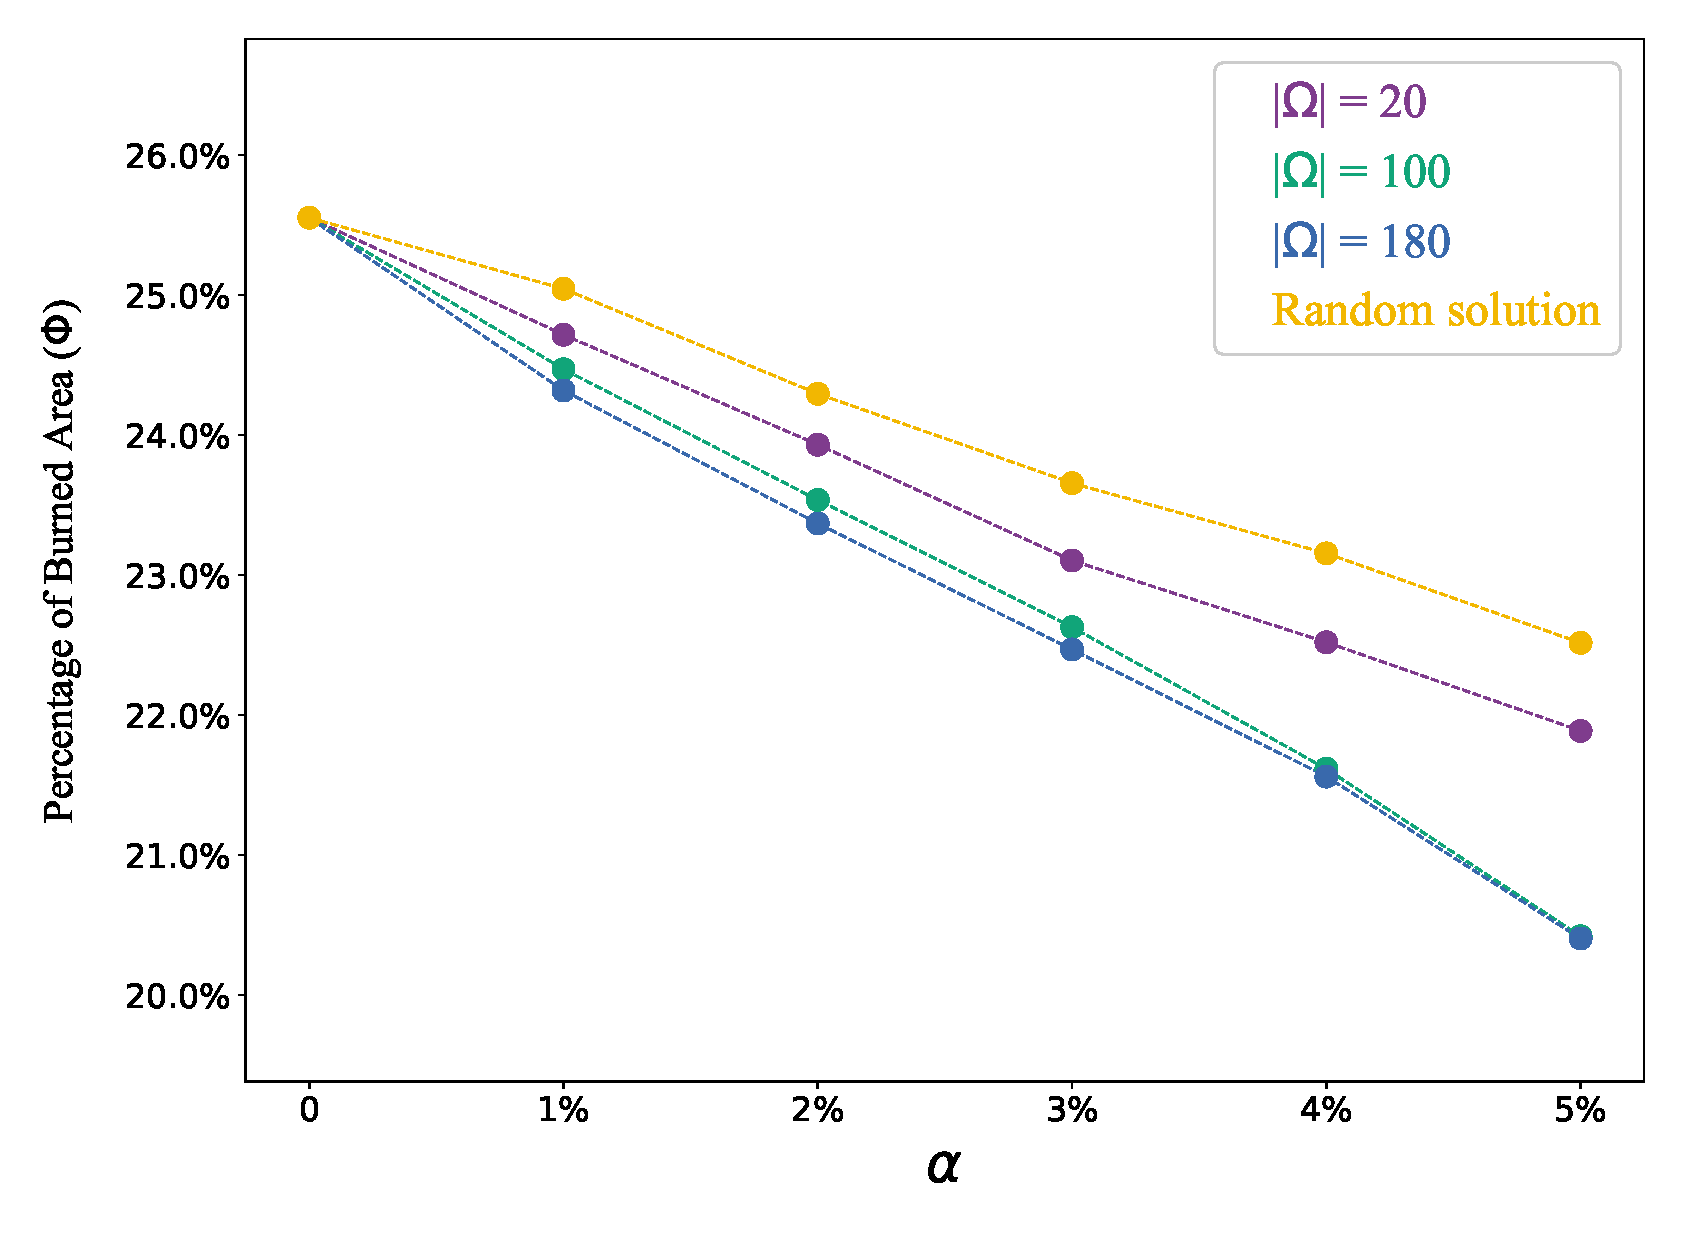
\includegraphics[width=0.9\linewidth]{figs/dinamic1000_1.eps}
    \caption{Average burned area by $|\Omega|$ for $\lambda = 1.0$.}
    %\vspace{1ex}
\end{subfigure}%%
\begin{subfigure}[b]{0.5\linewidth}
    \centering
    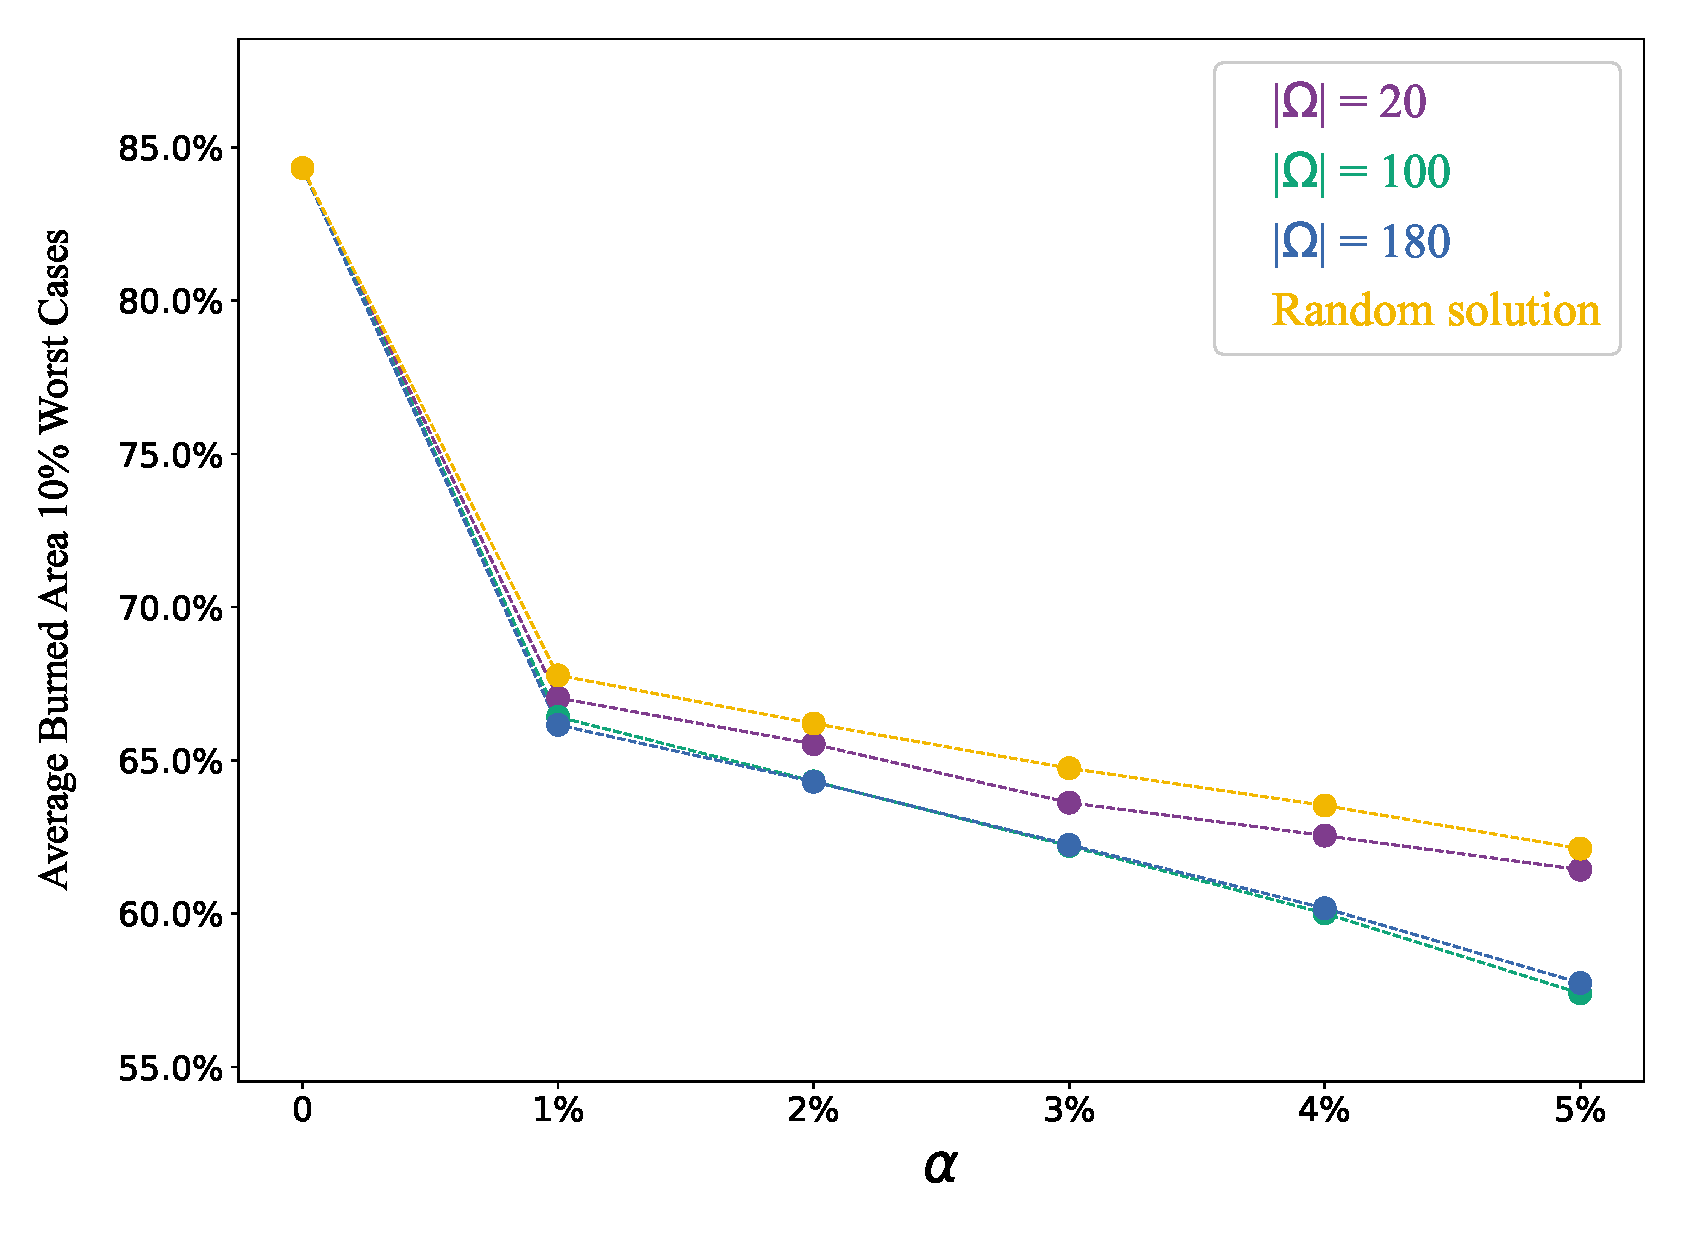
\includegraphics[width=0.9\linewidth]{figs/dinamic1000_2.eps}
    \caption{10\% worst case average by $|\Omega|$ for $\lambda = 1.0$}
    %\vspace{1ex}
  \end{subfigure} 
\begin{subfigure}[b]{0.5\linewidth}
    \centering
    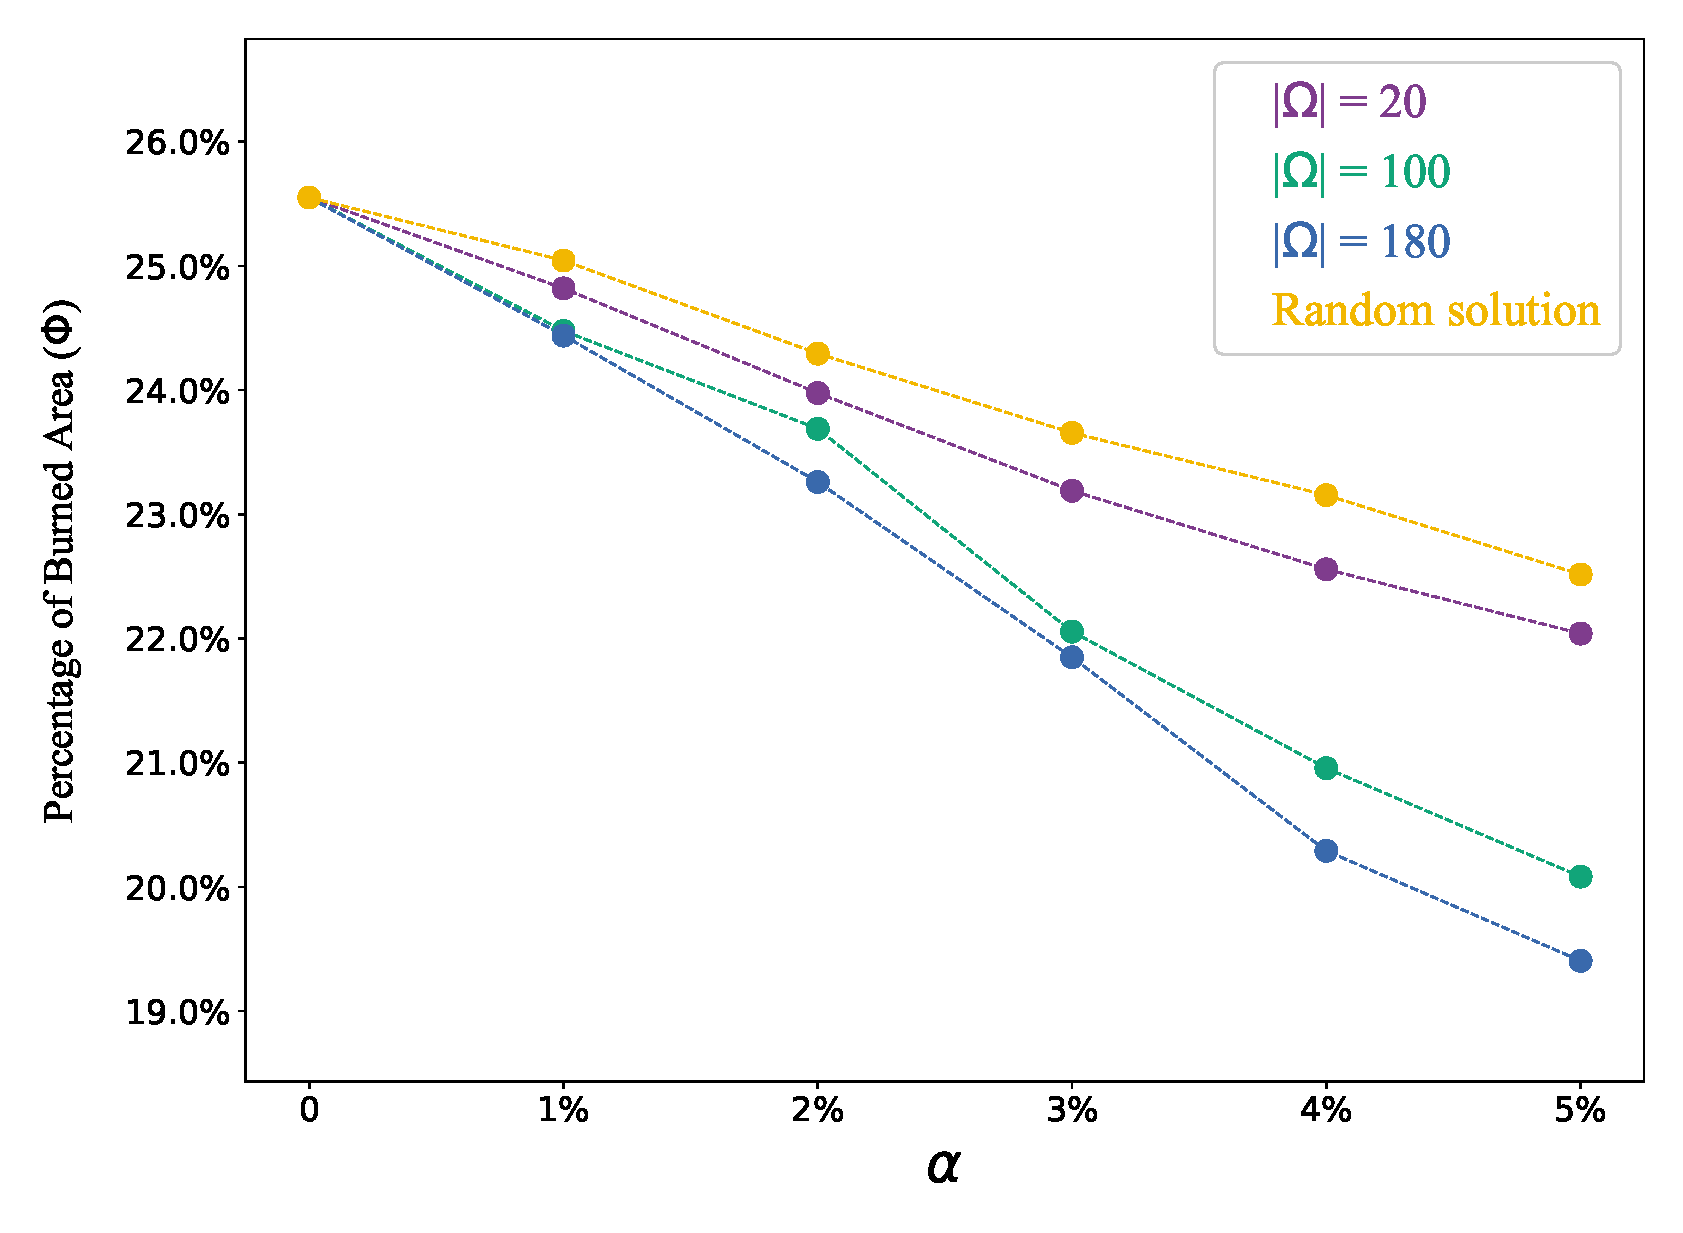
\includegraphics[width=0.9\linewidth]{figs/dinamic1000_3.eps}
    \caption{Average burned area by $|\Omega|$ for $\lambda = 0.5$.}
%    \vspace{1ex}
  \end{subfigure}%% 
\begin{subfigure}[b]{0.5\linewidth}
    \centering
    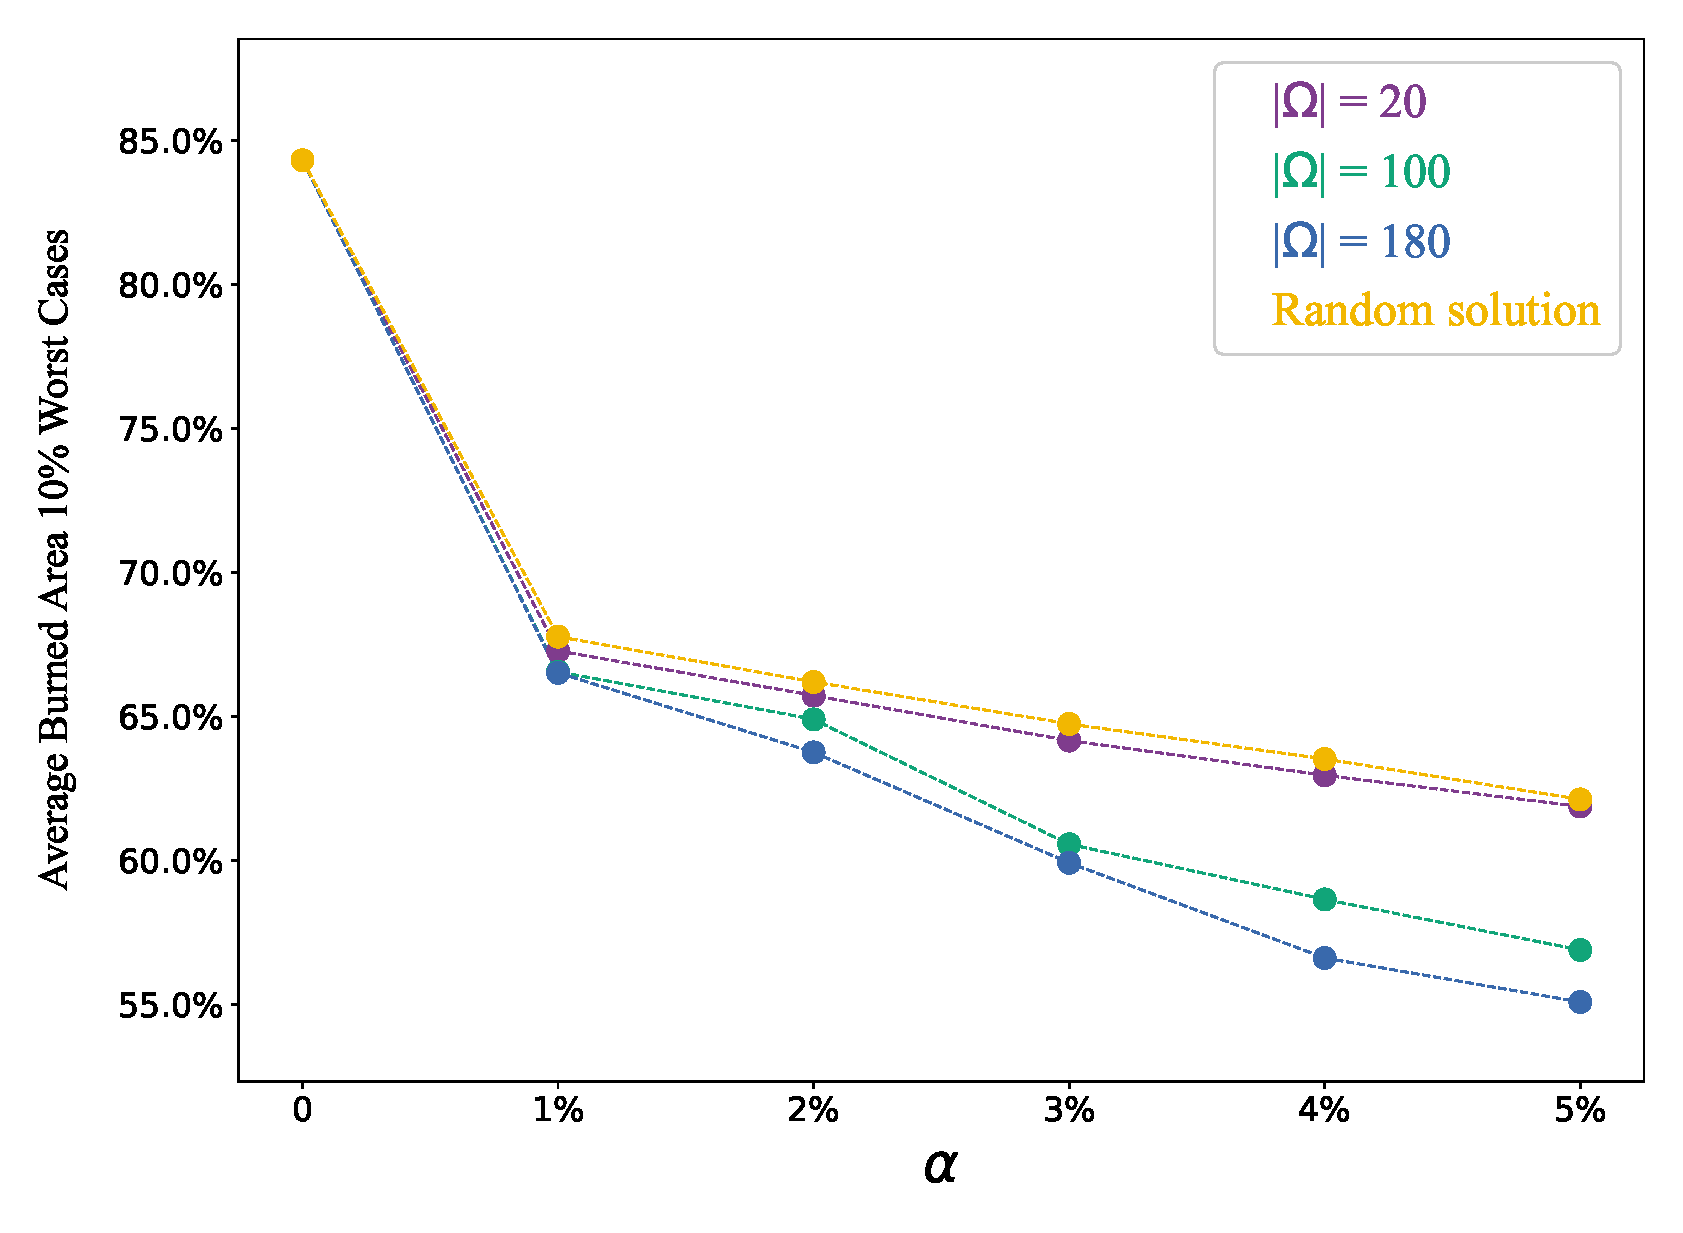
\includegraphics[width=0.9\linewidth]{figs/dinamic1000_4.eps}
    \caption{10\% worst case average by $|\Omega|$ for $\lambda = 0.5$.}
    %\vspace{1ex}
  \end{subfigure} 
\begin{subfigure}[b]{0.5\linewidth}
    \centering
    \captionsetup{justification=centering}
    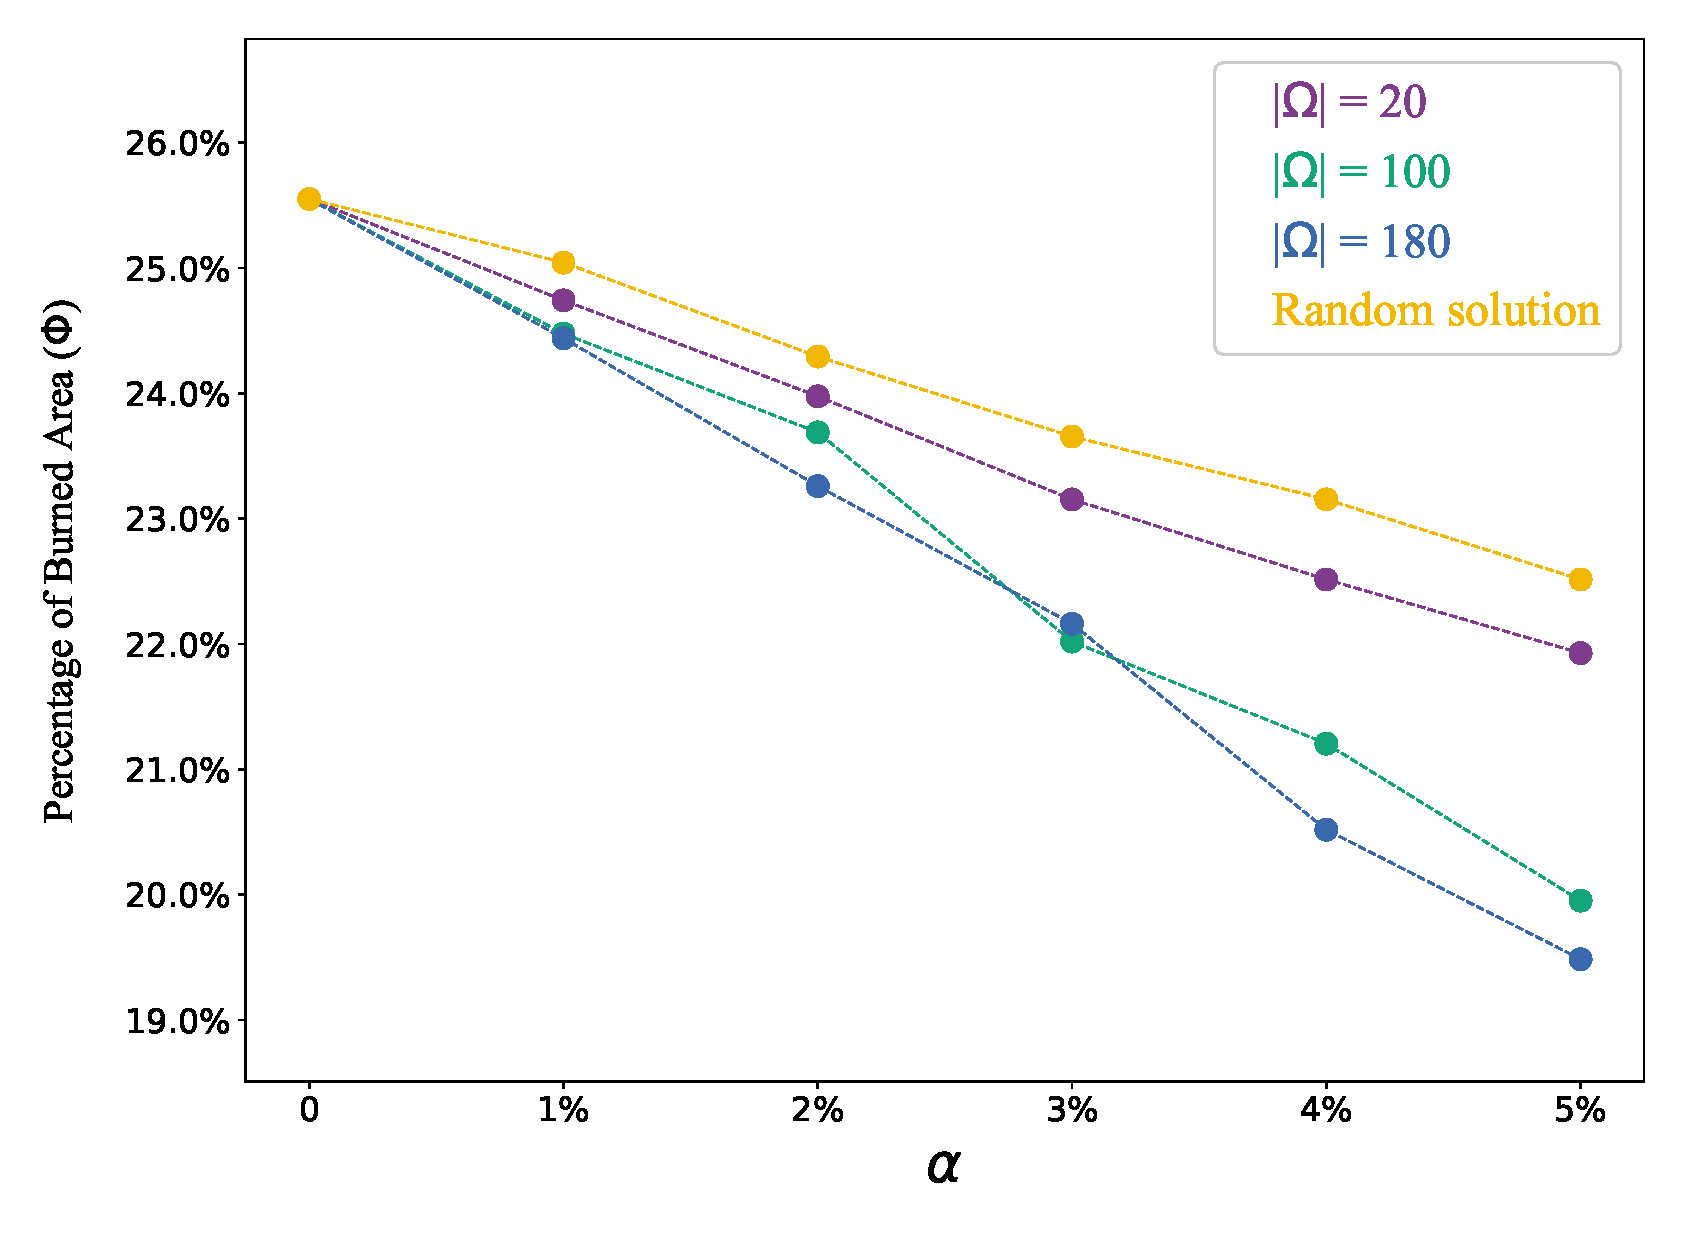
\includegraphics[width=0.9\linewidth]{figs/dinamic1000_5.eps}
    \caption{Average burned area by $\lvert \mathcal{S} \rvert$ for $\lambda = 0.0$.}
%    \vspace{1ex}
  \end{subfigure}%% 
\begin{subfigure}[b]{0.5\linewidth}
    \centering
    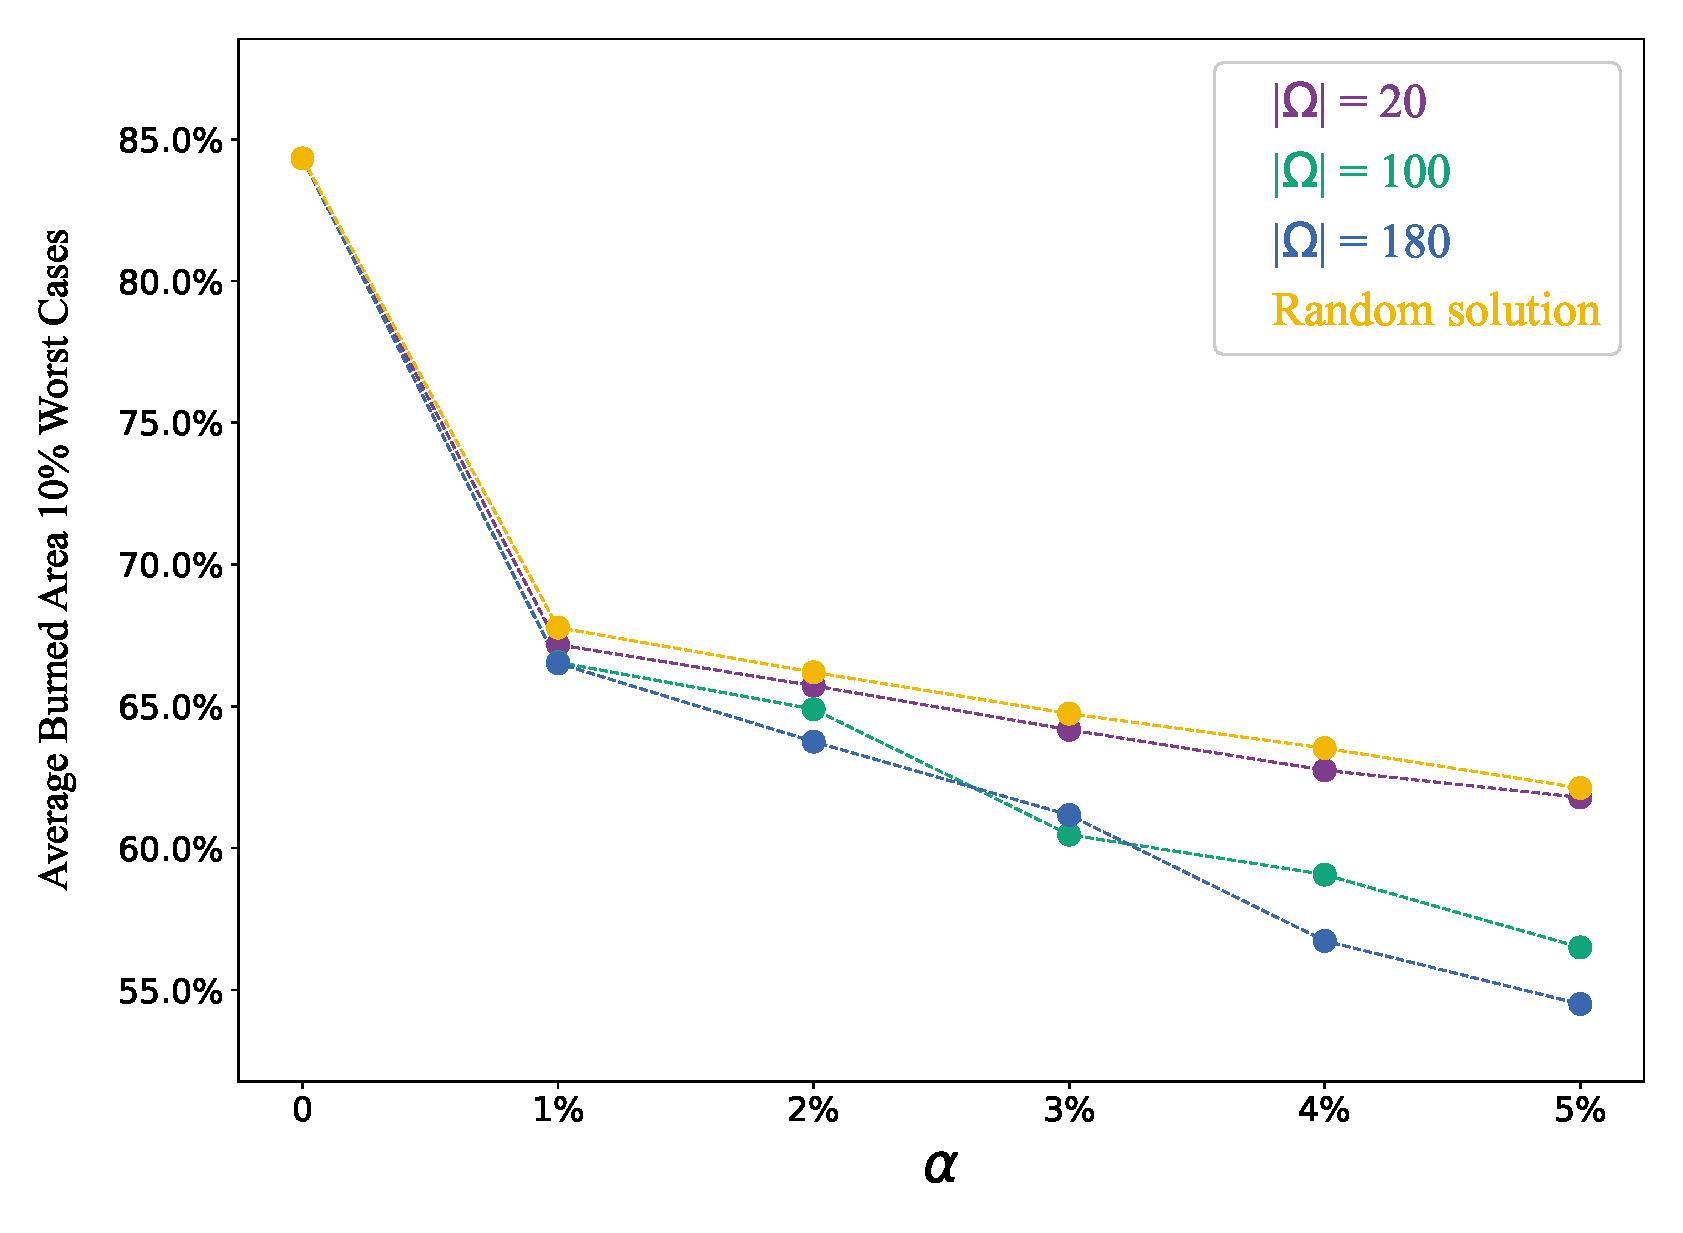
\includegraphics[width=0.9\linewidth]{figs/dinamic1000_6.eps}
    \caption{10\% worst case average by $\lvert \mathcal{S} \rvert$ for $\lambda = 0.0$}
    %\vspace{1ex}
  \end{subfigure} 
\caption{Evaluation of the solutions using C2F on 1,000 scenarios, $|\Omega|$ size assessment.}
\label{fig:evaluation}
\end{figure}

Figure\:\ref{fig:evaluation1} portrays the dynamic fire behavior when assessing the solutions derived from the stochastic program within the same set utilized for their formulation, i.e., $\texttt{C2F}(\vb{y}^*, \mathcal{S}, \lambda)$. An evaluation of the percentage of the burned area reveals that the solution for $\lambda = 1$ consistently exhibits superior performance across all values of $\alpha$, achieving an average reduction of nearly 7\%. When compared to the 20\% reduction showcased in Fig.\:\ref{fig:validationA}, it becomes evident that the alteration in fire behavior, induced by the introduction of a firebreak, leads to an increase in the burned area. This transformation that the stochastic solution serves as an approximation to the optimal placement when considering fire dynamics. Consequently, even though it does not capture the complete fire spread pattern, it still outperforms a random solution. A similar trend is observed for the average of the 10\% worst cases, with only a 15\% reduction in contrast to the almost 50\% reduction depicted in Fig.\:\ref{fig:validationB}. Regarding $\lambda$, the best results were obtained using $\lambda = 1$ for $\alpha = $2\% and 3\% and $\lambda = 0.5$ for $\alpha =$ 4\% and 5\%.

Nonetheless, the numerical results suggest the model's potential effectiveness, evaluating its performance on a diverse range of wildfires is crucial to account for the inherent uncertainty associated with fire behavior. For this, we assess the solution provided by the model through a simulation procedure based on the Cell2Fire simulator. Thus, the obtained solutions were evaluated $\texttt{C2F}(\vb{y}^*, \Omega, \lambda)$ using a different set of 1,000 ($\vert \Omega \rvert = 1,000$) random simulations of wildfires provided by Cell2Fire. The evaluation was conducted in the same forest as the validation, utilizing the same geographic and meteorological conditions but a different combination of these and initial ignition points, resulting in a different set of scenarios. This comprehensive assessment will provide a more accurate representation of the solution's actual capacity to mitigate forest fire damage during real incidents.

Figure\:\ref{fig:evaluation} illustrates the percentage of burned area and the average for the worst 10\% of cases for solutions derived from 20, 100, and 180 scenario instances, evaluated across various sets of scenarios. It is crucial to note that these scenarios are encompassed within larger set sizes; for instance, the 100-scenario set includes the 20-scenario set, and the 180-scenario set includes both the 20 and 100 scenarios.

The results indicate a distinction between the performance of the stochastic solution during the scenario construction phase and its performance in subsequent testing simulations. This underscores the importance of carefully selecting representative cases to construct robust stochastic solutions. Remarkably, the graph highlights a significant finding: the solutions derived from the 180-scenario instance perform at worst almost equal to other scenario sizes for all of $\alpha$ values and all $\lambda $ values when comparing the percentage of burned area and the average for the 10\% of worst cases. Nevertheless, the difference between the results for $|\Omega| = 100$ and $|\Omega| = 180$ are lower than between  $|\Omega| = 100$ and $|\Omega| = 20$, which suggests that the marginal gain for both measures decrease as the number of scenarios increases, thus, employing a scenario set of $|\Omega| = 100$ is sufficient to enhance the performance of lower-scenario instances and yield more robust solutions, even matching larger scenario set sizes in some instances.

Regarding $\lambda$, for both metrics, $\lambda = 0.5$ and $\lambda = 0.0$ exhibit similar behavior, performing slightly better than $\lambda = 1.0$ in terms of the percentage of burned area and the average of worst cases for scenario sizes of $|\Omega| = 100$ and $|\Omega| = 180$. Overall, the best results are obtained using $\lambda = 0.5$ and $|\Omega| = 180$, with slightly less favorable outcomes using $|\Omega| = 100$.

Regarding $\alpha$, the curves presented in this section indicate a clear potential for improvement when higher levels of the treated area are considered. Overall, the evaluation using different sets of scenarios confirms the model's potential effectiveness. The results demonstrate the robustness of the solution obtained from a larger number of scenarios while also highlighting the diminishing marginal benefit of increasing the scenario quantity.

When comparing these results with Figure\:\ref{fig:static_1000} it is possible to appreciate an increase in almost 9\% in burned area and nearly 30\% of the average of burned area for the 10\% of worst cases. This, as explained before, happens due to the ability of fire to react to firebreaks and search paths that will provoke larger fire scars.

\begin{comment}
 
\subsection{Computational analysis on larger forests}\label{s:results}

The preceding section has outlined the findings for the Sub20 forest. However, it is important to underscore that one of the objectives of this article is the application of the model to real-scale forest scenarios. In the subsequent section, we present the computational results for the Sub40 and Sub100 forest configurations, each evaluated under various parameter settings, specifically, $\alpha =$ {0.01, 0.03, 0.05}, $\lambda = 0.5$, $\beta = 0.9$, and a scenario set size of $|\Omega| = 100$.

% Please add the following required packages to your document preamble:
% \usepackage{booktabs}
% \usepackage{graphicx}

\begin{table}[h]
\caption{Computational time and MIPGAP by $\alpha$ and forest size.}
\label{tab:gap_time2}
%\resizebox{\textwidth}{!}{%
\begin{tabular}{rrrrrrrrrr}
\hline
\multicolumn{1}{l}{$\alpha$} & \multicolumn{1}{l}{Forest} & \multicolumn{1}{l}{\begin{tabular}[c]{@{}l@{}}C. Time {[}min{]}\end{tabular}} & \multicolumn{1}{l}{MIP$_{gap}$} & \multicolumn{1}{l}{Forest} & \multicolumn{1}{l}{\begin{tabular}[c]{@{}l@{}}C. Time {[}min{]}\end{tabular}} & \multicolumn{1}{l}{MIP$_{gap}$} \\ \hline
1\%                     &                            & 1440                                                                              & 13.3                                                                                                                                                    &                            & 1440                                                                              & 35.2                      \\
3\%                     & Sub40                      & 1440                                                                              & 32.9                                                                                                                                             & Sub100                     & 1440                                                                              & 19.5                      \\
5\%                     &                            & 1440                                                                              & 35.7                                                                                                                       &                            & 1440                                                                              & 5.9                      \\ \hline
\end{tabular}%
%}
\end{table}


The results, as illustrated in Table \ref{tab:gap_time2}, reveal a noteworthy increase in optimality gap compared to the Sub20 forest, even when the optimization program was allotted a time limit of 24 hours. This escalation in the optimality gap can be primarily attributed to the expansion of the forest's scale, which consequently entails a proliferation in the number of decision variables.
Furthermore, an observable trend in the results is the amplification of the optimality gap as the parameter $\alpha$ increases. This behavior is a consequence of the augmented complexity associated with the placement of additional firebreaks, as $\alpha$ directly governs the proportion of land designated for firebreaks.
Nevertheless, it is intriguing to note that, for the Sub\textcolor{brown}{4}0 and Sub100 scenarios, the $\texttt{MIP}_{gap}$ demonstrates a decrease as $\alpha$ increases. This phenomenon arises because $\alpha$ represents a percentage of the total land area rather than a fixed count of firebreaks. Thus, the number of firebreaks generated with $\alpha = 0.05$ for Sub40 is not equivalent to that for Sub100. Consequently, when the quantity of firebreaks surpasses a specific threshold, the decision process tends to become trivial due to the program's inherent capacity to contain any initial ignition point effectively.
In theory, this threshold is reached when the number of firebreaks equals eight times the cardinality of the scenario set ($\alpha \lvert \mathcal{V} \vert = |\Omega|$). This configuration theoretically ensures that the firebreaks can enclose every possible initial ignition point. However, in practice, this threshold is achieved with a smaller number of firebreaks due to the relative homogeneity in weather conditions and the improbability of a scenario set where the fire would simultaneously propagate in all eight conceivable directions from a given ignition node.
\end{comment} 

\textcolor{red}{Add the analysis of the frontier pareto.}

\section{Conclusions}\label{Sec:conclusions}
In this study, we introduce an innovative two-stage stochastic optimization model for the strategic placement of firebreaks, leveraging the spatially explicit scenarios generated by the Cell2Fire simulator. This addresses the inherent unpredictability associated with wildfire spread and behavior. Our proposal is capable of finding the optimal placement for a firebreak plan under the assumption of static fire behaviour and performs better than arbitrary configurations.

Our comprehensive computational analysis sheds light on the approach's robustness and efficacy. We have unveiled that balancing the expected damage (EV) against risk (CVaR) — particularly with a preference parameter of $\lambda=0.5$— significantly curtails the extent of the burn area, including in the most severe 10\% of cases. This balance illustrates the potential for a calculated approach to mitigate wildfire destruction effectively.

Further, our findings explain that while augmenting the number of firebreaks typically leads to a reduction in burned area, the benefits tend to decrease marginally beyond a certain threshold. This highlights the critical need for strategic placement over sheer quantity, considering environmental trade-offs such as carbon footprint and biodiversity impacts.

In addition, our proposed approach innovatively incorporates cell-specific weights within the model, empowering decision-makers to prioritize the protection of cells based on ecological value or proximity to human habitats. While the current experimental setup did not explore the nuances of this weighting parameter, it certainly opens up a vital avenue for future research. Analyzing how varying these weights impacts model outcomes can provide deeper understanding and more tailored strategies for wildfire management, particularly in areas of high conservation value or significant human interest.

Looking ahead, future research should delve into incorporating dynamic wildfire behavior into optimization models to enhance their practical applicability. Additionally, evaluating the model in a multi-period decision framework would account for the dynamic nature of forest landscapes, offering insights into the long-term strategic planning of firebreaks. In addition, to embed into evaluations the negative externalities produced by the treatments in the landscape, such as the impact on carbon emissions and reduction of biodiversity, among others.

From a computational perspective, the inclusion of additional scenarios contributes to improved results. However, the incremental advantages achieved become increasingly modest as the computational time required increases. This observation underscores the existence of a trade-off between the benefits of incorporating additional scenarios and the associated computational expenses. Therefore, future research should focus on developing algorithms that can effectively address larger landscapes and employ scenario-selective strategies to avoid unnecessary increases in the size of the optimization model.

In conclusion, our computational experiments have demonstrated the potential effectiveness of our mathematical model for firebreak placement in mitigating forest fire damage. This study shows that incorporating fire behavior software, such as Cell2Fire, proves to be a powerful tool by introducing actual fire spread dynamics into the optimization program. This integration enables selecting a highly effective firebreak placement configuration to face the challenging task of mitigating the spread of wildfires. Thus, the insights gained from our analysis of various scenarios and parameter settings contribute to understanding optimal firebreak allocation strategies. As we continue to refine and expand our understanding of this model, it holds promise for improving wildfire management strategies, ultimately minimizing the ecological, humanitarian, and economic impacts of wildfires.  


\section*{Acknowledgments}
This project has received funding from the European Union’s Horizon 2020 research and innovation program under grant agreement No 101037419 (\href{https://fire-res.eu}{FIRE-RES}) and the Complex Engineering Systems Institute (CONICYT-PIA-FB0816). \textbf{JC} acknowledges the support of the ANID through funding Postdoctoral Fondecyt project No 3210311. Also, the authors gratefully acknowledge the research support provided by Dicyt project 062217DG, Vicerrector\'ia de Investigaci\'on, Desarrollo e Innovaci\'on, Universidad de Santiago de Chile.


\clearpage
\appendix
\section{Appendix}
\begin{figure}[h]
\centering
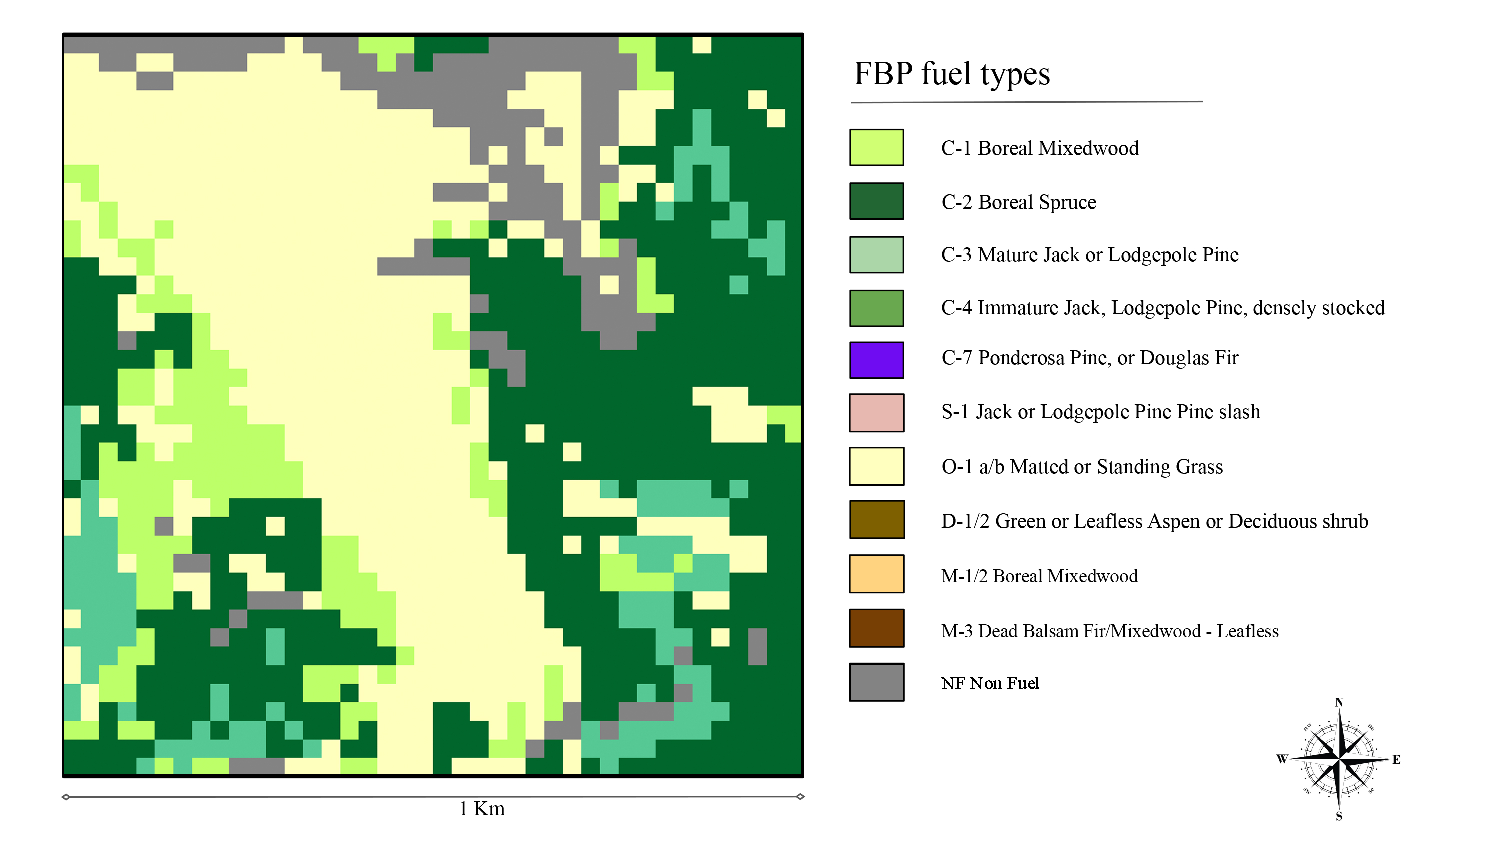
\includegraphics[scale=.5]{figs/sub40.pdf}
\caption{Sub40 Forest.}
\label{fig:Sub40}
\end{figure}

\begin{figure}[h]
\centering
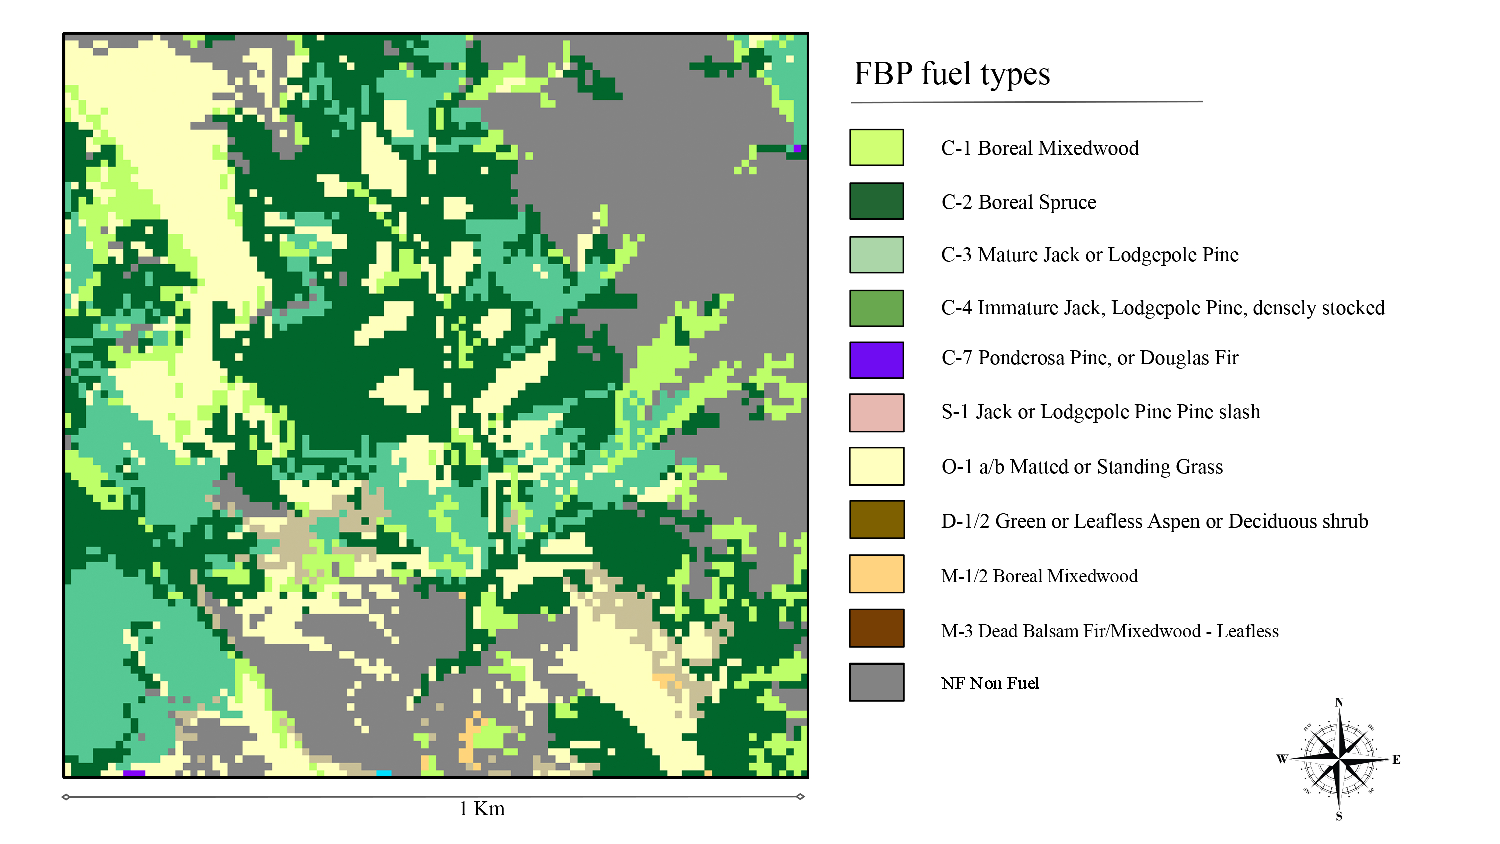
\includegraphics[scale=.5]{figs/sub100.pdf}
\caption{Sub100 Forest.}
\label{fig:Sub100}
\end{figure}

\clearpage
\bibliographystyle{cas-model2-names}

\bibliography{cas-refs}



\end{document}

